\chapter{\texorpdfstring{$^{39}\mathrm{\textbf{K}}(\MakeLowercase{p},\gamma)^{40}\mathrm{\textbf{C\MakeLowercase{a}}}$}{39K(p,g)40Ca} Constraints for Globular Cluster NGC 2419}
\label{ch:GC}

%%%%%%%%%%%%%%%%%%%%%%%%%%%%%%%%%%%%%%%%%%%%%%%%%%%%%%%%%%%%%%%%%%%%%%%%%%%%%%%%%%%%%%%%%%%%%
\section{Introduction}

% Globular clusters and anticorrelations in general (See Gratton et al. 2019)
%  3.1) Introduction to globular cluster abundance anticorrelations in general
%  - What is a globular cluster?
%  - Defined by multiple stellar populations (Bedin et al. 2004, Piotto 2007). Show the HR diagram for an example Milky Galaxy
%  - Defined by abundance anticorrelations. Show an example anticorrelation, such as O-Na
%  - Abundance anticorrelations result from pollution/mixing from older stars in the globular cluster (polluter stars) ["The (anti-)correlation among light elements is simply a manifestation of the multiple stellar populations." (Gratton et al. 2019)]
%  - Hydrogen burning in the polluter stars is the mechanism behind these anticorrelations (

This chapter details the original research constraining hydrogen-burning conditions responsible for abundance anomalies in globular clusters. In particular, the observed potassium enrichment and magnesium depletion in red giants of the globular cluster NGC 2419 is reproduced with nuclear reaction network calculations using new nuclear physics information presented in this chapter. A new reaction rate of the key potassium-destroying reaction, $^{39}\mathrm{K}(p,\gamma)^{40}\mathrm{Ca}$, is calculated from the new proton partial-widths and resonance energies of astrophysically-important, unbound $^{40}$Ca states measured in the proton-transfer reaction $^{39}\mathrm{K}(^{3}\mathrm{He},d)^{40}\mathrm{Ca}$. The reaction rate is significantly constrained for $T \lesssim 110$ MK. Monte Carlo network calculations will show new temperature-density constraints for hydrogen-burning, compared with that of the previously calculated reaction rate. Hot-bottom burning in Super-AGB stars is investigated as a polluter candidate driving the Mg--K anticorrelation in NGC 2419, as well as other abundance patterns involving potassium.

\section{Globular Clusters}

% From PRL (Before cutting material):
\begin{comment}
The abundance pattern of % (some)? b/c we understand the O-Na and Mg-Al ones pretty well 
globular clusters is still poorly understood, despite evidence of multiple stellar populations within each cluster \cite{Bedin2004,Piotto2007} and abundance anticorrelations of light element pairs between low-mass cluster stars, such as C--N, O--Na, and Mg--Al (see Gratton \emph{et al.} \cite{Gratton2012} for a recent review). The origin of these anticorrelations likely involves the currently observed globular cluster stars forming from the matter of earlier cluster stars, or \emph{polluter stars}, because the low-mass stars in which these anticorrelations have been observed do not produce sufficiently high temperatures to account for changes in abundance of the above elements.
%The origin of these anticorrelations likely involves matter mixing between stellar populations because the low-mass stars in which these anticorrelations have been observed do not produce sufficiently high temperatures to account for changes in abundance of the above elements. The currently observed globular cluster stars must therefore have been formed out of the polluted material from earlier globular cluster stars, or \emph{polluter stars}. 
The O--Na and Mg--Al abundance anticorrelations have been shown to be reproduced by low-temperature hydrogen burning at about 75 MK in the polluter stars of globular cluster NGC 6752 \cite{Prantzos2007}. However, the list of candidate sources for the polluter stars in NGC 6752, and for many other globular clusters, is quite long. % Cite them? 8 according to Iliadis et al. 2016
\end{comment}

Globular clusters are compact conglomerates of stars associated with all types of galaxies. They are typically on the order of 1 pc to a few tens of pc in radius. They are very old, in most cases having an age of about 10 Gyr, and they are also quite luminous, with a mean absolute visual magnitude $M_{V} = -7$. Peak globular cluster formation is thought to pre-date most stellar formation in galaxies, and they may have played a crucial role in early galaxy formation \cite{Gratton2019}. In the Milky Way galaxy, they often have low metallicity and are distributed throughout the halo, the thick disk, and the bulge. These properties, while interesting in their own right, are not what have made globular clusters garner considerable interest in the last few decades.

A characteristic recently attributed to globular clusters, which distinguishes them from similar objects such as open clusters, is the presence of chemical inhomogeneities among their low-mass stars. Once labeled \emph{abundance anomalies}, these inhomogeneities take the form of anticorrelations among the abundances of light element pairs, such as O--Na and Mg--Al. A new definition of globular clusters that includes this characteristic was suggested by Ref. \cite{Carretta2010}, since almost every globular cluster in which abundances have been observed has exhibited an O--Na anticorrelation. 
% ``In (almost) all studied GCs the Na-O anticorrelation has been found. One exception is Terzan 7, where no spread in O abundances has been found in the (only) seven stars observed by Sbordone et al. (2007), and may then be the most massive cluster observed so far without the Na-O anticorrelation. The other one is Pal 12, where Cohen (2004) finds very uniform O and Na abundances, but only for four stars." (Carretta et al. 2010).
% Sbordone, L., Bonifacio, P., Buonanno, R., et al. 2007, A&A, 465, 815
% Cohen, J. G. 2004, AJ, 127, 1545
The only exceptions are Terzan 7 and Pal 12, where the simultaneous Na and O abundances of only 7 \cite{Sbordone2007} and 4 \cite{Cohen2004} stars were observed, respectively. Other anticorrelations and correlations are exhibited in some, but not all globular clusters, making each cluster distinguishable by the combination and extent of their abundance inhomogeneities. These cluster-to-cluster differences are primarily driven by differences in luminosity and metallicity. Meanwhile, no anticorrelations have ever been observed in open clusters \cite{Gratton2019}.

Fig. \ref{fig:O-Na} shows the ubiquitous O--Na anticorrelation in 1,200 red giants among all 19 globular clusters sampled by Ref. \cite{Carretta2010}. The red giants with an enhanced Na abundance are associated with a depletion in O abundance, and vice versa. The populations of red giants are split into 3 categories based on the extent of their Na enrichment, and associated O depletion. These populations are the primordial (P), extreme (E), and intermediate (I) components, as indicated in the first panel of Fig. \ref{fig:O-Na}. The primordial population is Na-poor/O-rich, the extreme population is Na-rich/O-poor, and the intermediate population is in-between. The primordial population is so-called because the same abundance pattern is typical of field stars with a similar metallicity. However, the Na and O abundances of the intermediate and extreme populations indicates that these red giants went through an unknown process. Low-mass stars like red giants and main sequence stars do not reach the high temperatures necessary for the nucleosynthesis chains that produce the observed Na and O abundances. This reasoning also applies to the other observed anticorrelations in globular clusters \cite{Prantzos2007}.

\begin{figure}[t]
\centering
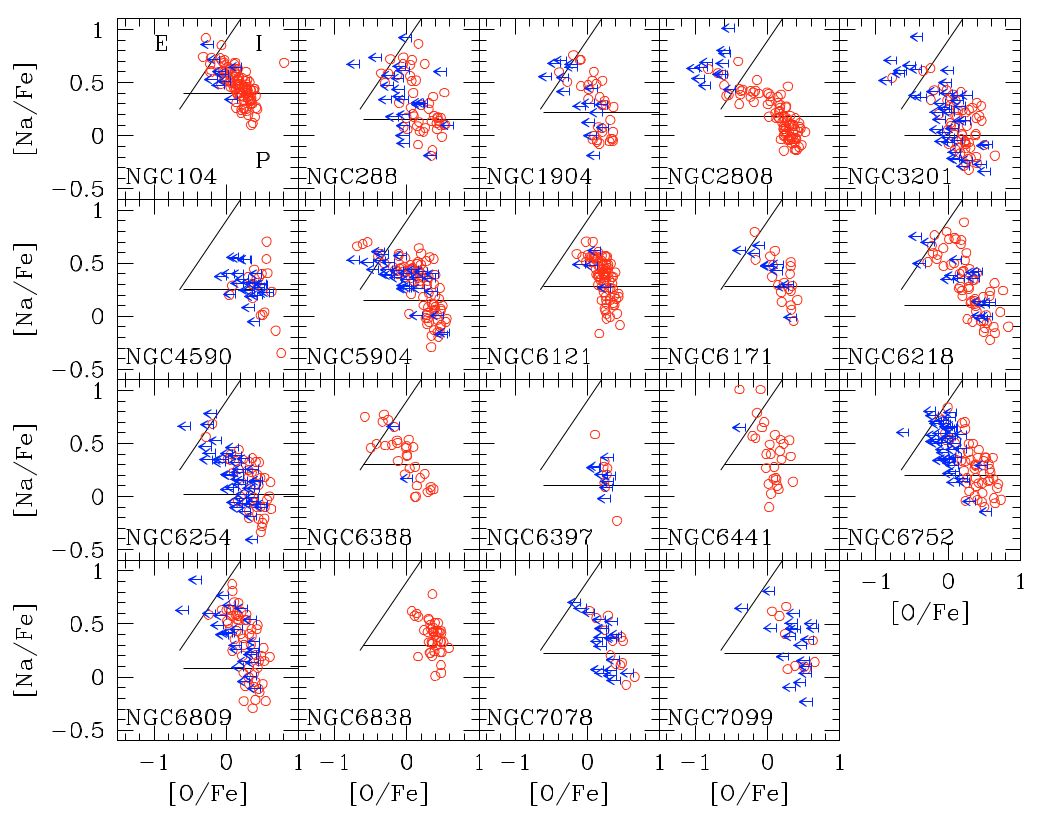
\includegraphics[width=6.5in]{Chapter-6/figs/O-Na.png}
\caption{\label{fig:O-Na}The O--Na anticorrelation of 1,200 red giants among all 19 globular clusters observed in the survey of Ref. \cite{Carretta2010}. Blue arrows indicate upper limits in O abundances, while lines separate different populations of red giants based on their relative O and Na richness. Primordial (P), extreme (E), and intermediate (I) populations are labeled in the first panel. See text for definitions of these populations. Adapted from \cite{Carretta2010}.}
\end{figure}

% PARAGRAPH 1: Cannot be in situ - must be mixing. Evidence for multiple stellar populations - pg 2 of Carretta2010 and Prantzos2007

% ``The (anti-)correlation among light elements is simply a manifestation of the multiple stellar populations." (Gratton et al. 2019) pg 12

% ``The variations are also found among unevolved stars currently on the main sequence (MS) of GCs (Gratton et al. 2001; Ramirez & Cohen 2002; Carretta et al. 2004; D’Orazi et al. 2010). This unequivocally implies that this composition has been imprinted in the gas by a previous generation of stars. The necessity of this conclusion stems from low-mass MS stars not being able to reach the high temperatures for the nucleosynthetic chains required to produce the observed inter-relations between the elements (in particular the Mg-Al anticorrelation). This calls for a class of now extinct stars, more massive than the low-mass ones presently evolving in GCs, as the site for the nucleosynthesis." (Carretta et al. 2010) pg 2

The most likely scenario explaining these inhomogeneities is that the currently observed stars are part of a second generation which formed from the ashes of an older, first generation of stars. The material ejected from these more-massive first generation stars upon their death likely polluted the inter-cluster medium where the second generation stars began to form. Hence, these first generation stars are sometimes called \emph{polluter stars}, a class of massive, extinct stars that are the origin of the apparent abundance anomalies. Different generations of stars exhisting in a given globular cluster would provide evidence for \emph{multiple stellar populations}. This premise has been widely debated over the last few decades, with most research supporting it at present \cite{Gratton2004,Gratton2012,Gratton2019}.

% PARAGRAPH 2: Mechanism of nucleosynthesis in second-generation globular cluster stars - H-burning. Type 1 vs type 2 globular clusters (different burning temperatures). - pg 12 of Gratton2019 - Cites Denisenkov and Denisenkova 1989; Langer et al. 1993
% Denisenkov PA, Denisenkova SN (1989) Possible explanation of the correlation between nitrogen and sodium over abundances for red giants in globular clusters. Astron Tsirkulyar 1538:11
% Langer GE, Hoffman R, Sneden C (1993) Sodium–oxygen abundance anticorrelations and deep-mixing scenarios for globular-cluster giants. Publ Astron Soc Pac 105:301–307. https://doi.org/10.1086/133147

Polluter stars are likely the site of the nucleosynthesis that gives rise to the currently observed abundance patterns in globular clusters. Their exact nature is unknown, but the nucleosynthesis mechanism driving the inhomogeneities in the vast majority of globular clusters is well established as proton-capture reactions in high temperature hydrogen-burning environments \cite{Denisenkov1989,Langer1993}. The ubiquitous O--Na anticorrelation, for example, is exhibited in the hydrogen burning of the CNO and Ne--Na cyles at about 40 MK \cite{Gratton2019}. Fig. \ref{fig:CNO_NeNa} shows the nucleosynthesis chains that lead to an overall oxygen depletion and sodium production. The first stage of the CNO cycle involves a series of $(p, \gamma)$ and $(\beta^{+}\nu)$ reactions on stable and radioactive nuclei, respectively, starting from $^{12}$C. This stage occurs at fusion temperatures of about 10 MK. Once $^{15}$N is reached, $^{15}\mathrm{N}(p, \alpha)^{12}\mathrm{C}$ will reset the cycle if the temperature is less than about 40 MK. Otherwise, the second stage of the CNO cycle will be activated from $^{15}\mathrm{N}(p, \gamma)^{16}\mathrm{O}$. This eventually leads to $^{17}$O, which resets the cycle via $^{17}\mathrm{O}(p, \alpha)^{14}\mathrm{N}$. This second stage leads to an overall destruction of oxygen. Meanwhile, the Ne--Na cycle activates at about 40 MK as well, starting from $^{20}\mathrm{Ne}(p, \gamma)^{21}\mathrm{Na}$. Once $^{23}$Na is reached, it will reset the cycle via $^{23}\mathrm{Na}(p, \alpha)^{20}\mathrm{Ne}$ if temperatures are less than about 70 MK, otherwise $^{23}\mathrm{Na}(p, \gamma)^{24}\mathrm{Mg}$ is activated. These destruction reactions on $^{23}$Na are slow enough such that sodium is produced overall.

\def\BoxSpace{0.3} % Defining the variable BoxSpace to value in brackets
\def\BoxSpacetwo{\BoxSpace * 2} % So I don't have to keep doing {2+(\BoxSpace * 2)}
\def\BoxSpacethree{\BoxSpace * 3}
\def\BoxSpacehalf{\BoxSpace * 0.5}
\def\AOS{0.2} % Arrow Offset
\def\AW{0.52} % Arrow Width (mm)
\usetikzlibrary{arrows, arrows.meta}

\begin{figure}[t]
\centering
\noindent
\begin{minipage}{.44\linewidth}
\begin{tikzpicture}[scale=1.5, every node/.style={transform shape}]

% (0,0) is at the bottom left corner of plot, where 12C is
\filldraw[fill = light-gray] (0,0) rectangle (1,1); % 12C box
\filldraw[fill = light-gray] (1+\BoxSpace,0) rectangle (2+\BoxSpace,1); % 13C box
%\draw (2+\BoxSpacetwo,0) rectangle (3+\BoxSpacetwo,1); % 14C box
\draw (0,1+\BoxSpace) rectangle (1,2+\BoxSpace); % 13N box
\filldraw[fill = light-gray] (1+\BoxSpace,1+\BoxSpace) rectangle (2+\BoxSpace,2+\BoxSpace); % 14N box
\filldraw[fill = light-gray] (2+\BoxSpacetwo,1+\BoxSpace) rectangle (3+\BoxSpacetwo,2+\BoxSpace); % 15N box
%\draw (0,2+\BoxSpacetwo) rectangle (1,3+\BoxSpacetwo); % 14O box
\draw (1+\BoxSpace,2+\BoxSpacetwo) rectangle (2+\BoxSpace,3+\BoxSpacetwo); % 15O box
\filldraw[fill = light-gray] (2+\BoxSpacetwo,2+\BoxSpacetwo) rectangle (3+\BoxSpacetwo,3+\BoxSpacetwo); % 16O box
\filldraw[fill = light-gray] (3+\BoxSpacethree,2+\BoxSpacetwo) rectangle (4+\BoxSpacethree,3+\BoxSpacetwo); % 17O box
\draw (2+\BoxSpacetwo,3+\BoxSpacethree) rectangle (3+\BoxSpacetwo,4+\BoxSpacethree); % 17F box

\node[text=blue] at (0.5,0.5) {$^{12}\mathrm{C}$};
\node[text=red] at (1+\BoxSpace+0.5,0.5) {$^{13}\mathrm{C}$};
\node at (0.5,1+\BoxSpace+0.5) {$^{13}\mathrm{N}$};
\node[text=red] at (1+\BoxSpace+0.5,1+\BoxSpace+0.5) {$^{14}\mathrm{N}$};
\node at (2+\BoxSpacetwo+0.5,1+\BoxSpace+0.5) {$^{15}\mathrm{N}$};
\node at (1+\BoxSpace+0.5,2+\BoxSpacetwo+0.5) {$^{15}\mathrm{O}$};
\node[text=blue] at (2+\BoxSpacetwo+0.5,2+\BoxSpacetwo+0.5) {$^{16}\mathrm{O}$};
\node at (3+\BoxSpacethree+0.5,2+\BoxSpacetwo+0.5) {$^{17}\mathrm{O}$};
\node at (2+\BoxSpacetwo+0.5,3+\BoxSpacethree+0.5) {$^{17}\mathrm{F}$};

\draw[line width = \AW mm, -{Triangle[]}] (0.5,1-\AOS) -- (0.5,1+\BoxSpace+\AOS); % 12C(p,g)
\draw[line width = \AW mm, -{Triangle[]}] (1-\AOS,1+\BoxSpace+\AOS) -- (1+\BoxSpace+\AOS, 1-\AOS); % 13N(B+)
\draw[line width = \AW mm, -{Triangle[]}] (1+\BoxSpace+0.5,1-\AOS) -- (1+\BoxSpace+0.5,1+\BoxSpace+\AOS); % 13C(p,g)
\draw[line width = \AW mm, -{Triangle[]}] (1+\BoxSpace+0.5,2+\BoxSpace-\AOS) -- (1+\BoxSpace+0.5,2+\BoxSpacetwo+\AOS); % 14N(p,g)
\draw[line width = \AW mm, -{Triangle[]}] (2+\BoxSpace-\AOS,2+\BoxSpacetwo+\AOS) -- (2+\BoxSpacetwo+\AOS,2+\BoxSpace-\AOS); % 15O(B+)
\draw[line width = \AW mm, -{Triangle[]}, dashed] (2+\BoxSpacetwo+\AOS,1+\BoxSpace+\AOS) -- (1-\AOS,1-\AOS); % 15N(p,a)

\draw[line width = \AW mm, -{Triangle[]}, dashed] (2+\BoxSpacetwo+0.5,2+\BoxSpace-\AOS) -- (2+\BoxSpacetwo+0.5,2+\BoxSpacetwo+\AOS); %15N(p,g)
\draw[line width = \AW mm, -{Triangle[]}] (2+\BoxSpacetwo+0.5,3+\BoxSpacetwo-\AOS) -- (2+\BoxSpacetwo+0.5,3+\BoxSpacethree+\AOS); %16O(p,g)
\draw[line width = \AW mm, -{Triangle[]}] (3+\BoxSpacetwo-\AOS,3+\BoxSpacethree+\AOS) -- (3+\BoxSpacethree+\AOS,3+\BoxSpacetwo-\AOS); %17F(B+)
\draw[line width = \AW mm, -{Triangle[]}] (3+\BoxSpacethree+\AOS,2+\BoxSpacetwo+\AOS) -- (2+\BoxSpace-\AOS,2+\BoxSpace-\AOS); %17O(p,a)
\end{tikzpicture}
\end{minipage}
%
\begin{minipage}{.44\linewidth} \hfill
\centering
\noindent
\begin{tikzpicture}[scale=1.5, every node/.style={transform shape}]

\filldraw[fill = light-gray] (0,0) rectangle (1,1); % 20Ne box
\filldraw[fill = light-gray] (1+\BoxSpace,0) rectangle (2+\BoxSpace,1); % 21Ne box
\filldraw[fill = light-gray] (2+\BoxSpacetwo,0) rectangle (3+\BoxSpacetwo,1); % 22Ne box
\draw (0,1+\BoxSpace) rectangle (1,2+\BoxSpace); % 21Na Box
\draw (1+\BoxSpace,1+\BoxSpace) rectangle (2+\BoxSpace,2+\BoxSpace); % 22Na Box
\filldraw[fill = light-gray] (2+\BoxSpacetwo,1+\BoxSpace) rectangle (3+\BoxSpacetwo,2+\BoxSpace); % 23Na Box
\filldraw[fill = light-gray] (2+\BoxSpacetwo,2+\BoxSpacetwo) rectangle (3+\BoxSpacetwo,3+\BoxSpacetwo); %24Mg Box

\node[text=blue] at (0.5,0.5) {$^{20}\mathrm{Ne}$};
\node at (1+\BoxSpace+0.5,0.5) {$^{21}\mathrm{Ne}$};
\node at (2+\BoxSpacetwo+0.5,0.5) {$^{22}\mathrm{Ne}$};
\node at (0.5,1+\BoxSpace+0.5) {$^{21}\mathrm{Na}$};
\node at (1+\BoxSpace+0.5,1+\BoxSpace+0.5) {$^{22}\mathrm{Na}$};
\node[text=red] at (2+\BoxSpacetwo+0.5,1+\BoxSpace+0.5) {$^{23}\mathrm{Na}$};
\node at (2+\BoxSpacetwo+0.5,2+\BoxSpacetwo+0.5) {$^{24}\mathrm{Mg}$};

\draw[line width = \AW mm, -{Triangle[]}] (0.5,1-\AOS) -- (0.5,1+\BoxSpace+\AOS); %20Ne(p,g)
\draw[line width = \AW mm, -{Triangle[]}] (1-\AOS,1+\BoxSpace+\AOS) -- (1+\BoxSpace+\AOS,1-\AOS); % 21Na(B+)
\draw[line width = \AW mm, -{Triangle[]}] (1+\BoxSpace+0.5,1-\AOS) -- (1+\BoxSpace+0.5,1+\BoxSpace+\AOS); %21Ne(p,g)
\draw[line width = \AW mm, -{Triangle[]}] (2+\BoxSpace-\AOS,1+\BoxSpace+\AOS) -- (2+\BoxSpacetwo+\AOS,1-\AOS); %22Na(B+)
\draw[line width = \AW mm, -{Triangle[]}] (2+\BoxSpacetwo+0.5,1-\AOS) -- (2+\BoxSpacetwo+0.5,1+\BoxSpace+\AOS); %22Ne(p,g)
\draw[line width = \AW mm, -{Triangle[]},dashed] (2+\BoxSpacetwo+0.5,2+\BoxSpace-\AOS) -- (2+\BoxSpacetwo+0.5,2+\BoxSpacetwo+\AOS); %23Na(p,g)
\draw[line width = \AW mm, -{Triangle[]},dashed] (2+\BoxSpacetwo+\AOS,1+\BoxSpace+\AOS) -- (1-\AOS,1-\AOS); %23Na(p,a)20Ne

\end{tikzpicture}
\end{minipage}
\vspace{0.75 cm}
\caption{\label{fig:CNO_NeNa}The hydrogen burning mechanism driving the O--Na anticorrelation. Nuclei in blue are destroyed overall in the various cycles, while nuclei in red are produced. Shaded nuclei are stable. The first two stages of the CNO cycle (left), distinguished by the temperature-dependent branch at $^{15}$N, lead to an overall depletion of oxygen. The $^{15}\mathrm{N}(p, \gamma)^{16}\mathrm{O}$ reaction is activated at about 40 MK. The Ne--Na cycle (right), occurring simultaneously at about the same activation temperature, leads to an overall production of sodium. The $^{23}\mathrm{Na}(p,\gamma)^{24}\mathrm{Mg}$ reaction activates at about 70 MK.}
\end{figure}

% PARAGRAPH 3: Dilution model - mix of pristine and processed matter - pg 14 of Gratton2019

Although nucleosynthesis via hydrogen burning is what drives the observed abundance patterns, it is not the only mechanism responsible for them. The majority of second generation stars must be composed of a mixture of nuclear-processed ejecta and matter with a pristine composition, in order for nuclear reaction network models to reproduce the observed globular cluster abundance patterns \cite{Prantzos2007}. The nuclear-processed ejecta is the matter resulting from nucleosynthesis via hydrogen burning in the first generation polluter stars, while pristine matter refers to the unprocessed gas left behind from the first burst of star formation. Many polluter star sites such as AGB stars, fast-rotating massive stars, and supermassive stars require dilution with unprocessed gas in order to convert their correlated O and Na abundances into the observed anticorrelation \cite{DErcole2010,DErcole2011,DErcole2012}. The observed, mixed abundances in a typical dilution model are obtained by diluting one part of processed matter with $f$ parts of pristine matter, as in
\begin{equation}
X_{\mathrm{mix}} = \frac{X_{\mathrm{proc}} + f X_{\mathrm{pris}}}{1 + f},
\end{equation}
where $X$ is the mass fraction of a given nuclide among its specific composition and $f$ is the dilution factor \cite{Prantzos2007,Carretta2009}. A very small dilution factor represents nearly pure processed matter, while a very large dilution factor results in mostly pristine matter. The dilution model works very well for most globular clusters, but often a single dilution model does not simultaneously reproduce the abundances of the extreme and intermediate populations. In these cases, more than one class of polluter stars is required to match the observations, suggesting that the multiple populations premise may be more complex than previously considered \cite{Gratton2019}.

% PARAGRAPH 4?? (Skip this): Mass-budget problem - pg 15 of Gratton2019

%%%%%%%%%%%%%%%%%%%%%%%%%%%%%%%%%%%%%%%%%%%%%%%%%%%%%%%%%%%%%%%%%%%%%%%%%%%%%%%%%%%%%%%%%%%%%
\section{NGC 2419 and the Mg--K Anticorrelation} \label{sec:NGC2419}
% Iliadis et al. 2016
% Derhmingny et al. 2017

% PARAGRAPH 1: Mg-K abundance observations (2012)

% The globular cluster NGC 2419, imaged by the Hubble Space Telescope in Fig. \ref{fig:NGC2419}, was recently found to exhibit some puzzling abundance patterns.

While the O--Na anticorrelation is ubiquitous in globular clusters, there are other abundance patterns that are unique to individual or a small subset of globular clusters. The globular cluster NGC 2419 was recently found to exhibit some puzzling abundance patterns. About 30$\%$ of the red giants observed show a strong K enrichment correlated with a considerable Mg depletion \cite{Mucciarelli2012,Cohen2012}. Fig. \ref{fig:MgK} shows the observed elemental potassium and magnesium abundances, with respect to iron, for the red giants in NGC 2419 sampled by Ref. \cite{Mucciarelli2012} in red and Ref. \cite{Cohen2012} in blue. This was the first discovery of a Mg--K anticorrelation in any globular cluster. Only one other cluster to date, NGC 2808, has exhibited such an anticorrelation in a small portion of its stars \cite{Mucciarelli2015,Mucciarelli2017}, but the extent of the K enrichment is about 7 times less than that of NGC 2419. Meanwhile, the extent of the Mg depletion is about 3 times less. The evolutionary history of NGC 2419 must therefore be rather unique for it to exhibit such abundance patterns not seen in other globular clusters.

%\begin{figure}[t]
%\centering
%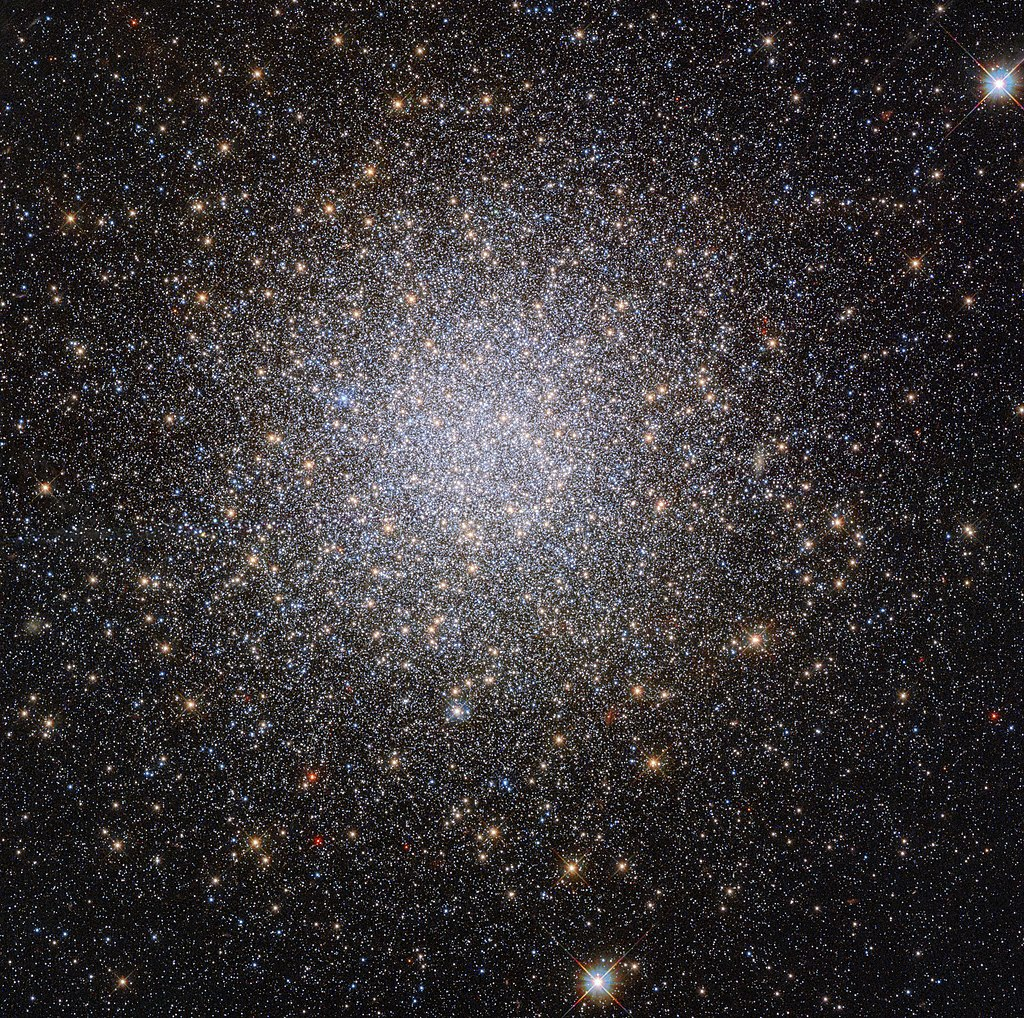
\includegraphics[width=3in]{Chapter-6/figs/NGC2419.jpg}
%\caption{\label{fig:NGC2419}An image of the globular cluster NGC 2419 taken by the Hubble Space Telescope \cite{NGC2419Hubble,Larsen2019}.}
%\end{figure}

\begin{figure}[t]
\centering
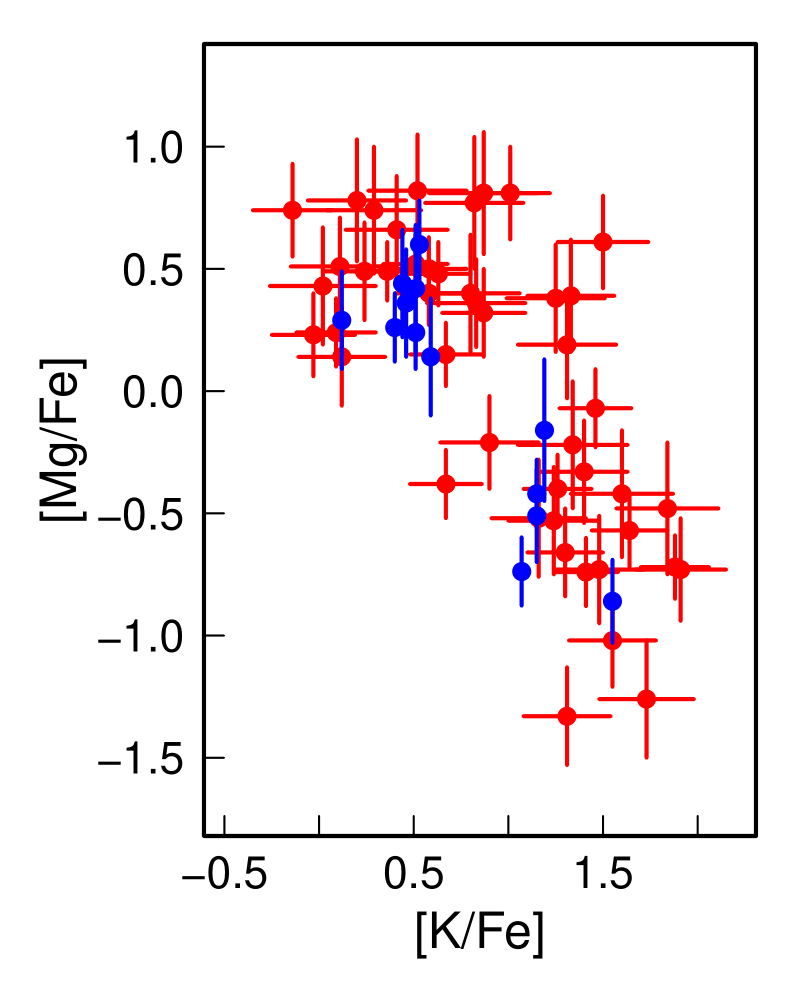
\includegraphics[width=2.5in]{Chapter-6/figs/MgK_Observation.png}
\caption{\label{fig:MgK}The observed Mg and K elemental abundances of red giants in NGC 2419 from Refs. \cite{Mucciarelli2012} (red) and \cite{Cohen2012} (blue). Figure adapted from \cite{Iliadis2016}.}
\end{figure}

% PARAGRAPH 2: Reaction network leading to K abundance (from 36Ar to 39K)

Just as the nucleosynthesis mechanism for the O--Na anticorrelation involves a series of $(p,\gamma)$ reactions and radioactive decays, the same is true for the Mg-K anticorrelation. The hydrogen burning schemes are illustrated in Fig. \ref{fig:MgKHBurning}. The Mg--Al cycle, shown on the left-hand side of the figure, starts from $^{24}$Mg at about 70 MK. After the subsequent $^{24}\mathrm{Mg}(p,\gamma)^{25}\mathrm{Al}$ and $^{25}\mathrm{Al}(\beta^{+}\nu)^{25}\mathrm{Mg}$ reactions, there is a chance the $^{26}\mathrm{Al}^{m}$ isomer is populated. The isomer preferrentially $\beta^{+}$ decays to $^{26}$Mg, while the ground state $^{26}\mathrm{Al}^{g}$ preferrentially captures a proton. Either scenario eventually synthesizes $^{27}$Al, which can repeat the cycle with $^{27}\mathrm{Al}(p,\alpha)^{24}\mathrm{Mg}$ or proceed with $^{27}\mathrm{Al}(p,\gamma)^{28}\mathrm{Si}$ if the temperature is more than about 80 MK. The overall effect is a depletion of magnesium and an enrichment of aluminum and silicon.

The hydrogen burning scheme for the K enrichment in NGC 2419 is illustrated on the right-hand side of Fig. \ref{fig:MgKHBurning}. It has been shown to start from $^{36}$Ar, an $\alpha$-nucleus and the most abundant argon isotope at the low metallicities of the first stellar generation \cite{Ventura2012}. Some authors \cite{Ventura2012,Mucciarelli2015} have incorrectly claimed that the main K enrichment chain involves the decay of $^{37}$Ar to $^{37}$Cl, then the subsequent $^{37}\mathrm{Cl}(p,\gamma)^{38}\mathrm{Ar}$ reaction, indicated by the dashed arrows in Fig. \ref{fig:MgKHBurning}. However, as Ref. \cite{Iliadis2016} indicates, the $^{37}\mathrm{Ar}(p,\gamma)^{38}\mathrm{K}$ reaction has a much larger decay constant than the electron capture reaction $^{37}\mathrm{Ar}(e^{-}, \nu)^{37}\mathrm{Cl}$ at the stellar densities of interest. Therefore, the main chain must proceed to $^{38}$K before the subsequent $^{38}\mathrm{K}(\beta^{+}\nu)^{38}\mathrm{Ar}$ and $^{38}\mathrm{Ar}(p,\gamma)^{39}\mathrm{K}$ reactions. The former chain is expected to contribute only marginally to $^{39}$K nucleosynthesis. Additionally, unlike the mechanisms for the O--Na anticorrelation and the Mg depletion, the sequence leading from $^{36}$Ar to $^{39}$K is not a cycle because the $^{39}\mathrm{K}(p,\alpha)^{36}\mathrm{Ar}$ reaction has a much smaller decay constant than $^{39}\mathrm{K}(p,\gamma)^{40}\mathrm{Ca}$. However, as it will become clear in Section \ref{sec:NGC2419}, the $^{39}\mathrm{K}(p,\gamma)^{40}\mathrm{Ca}$ reaction rate is currently very uncertain in the astrophysical temperature range of interest.

\begin{figure}[t]
\centering
\noindent
\begin{minipage}{.44\linewidth}
\begin{tikzpicture}[scale=1.5, every node/.style={transform shape}]

% (0,0) is at the bottom left corner of plot, where 24Mg is.
\filldraw[fill = light-gray] (0,0) rectangle (1,1); % 24Mg box
\filldraw[fill = light-gray] (1+\BoxSpace,0) rectangle (2+\BoxSpace,1); % 25Mg box
\filldraw[fill = light-gray] (2+\BoxSpacetwo,0) rectangle (3+\BoxSpacetwo,1); % 26Mg box
\draw (0,1+\BoxSpace) rectangle (1,2+\BoxSpace); % 25Al box
\draw (1+\BoxSpace,1+\BoxSpace) rectangle (2+\BoxSpace,2+\BoxSpace); % 26Al box
\filldraw[fill = light-gray] (2+\BoxSpacetwo,1+\BoxSpace) rectangle (3+\BoxSpacetwo,2+\BoxSpace); % 27Al box
\draw (1+\BoxSpace,2+\BoxSpacetwo) rectangle (2+\BoxSpace,3+\BoxSpacetwo); % 27Si box
\filldraw[fill = light-gray] (2+\BoxSpacetwo,2+\BoxSpacetwo) rectangle (3+\BoxSpacetwo,3+\BoxSpacetwo); % 28Si box

\node[text=blue] at (0.5,0.5) {$^{24}\mathrm{Mg}$};
\node at (1+\BoxSpace+0.5,0.5) {$^{25}\mathrm{Mg}$};
\node at (2+\BoxSpacetwo+0.5,0.5) {$^{26}\mathrm{Mg}$};
\node at (0.5,1+\BoxSpace+0.5) {$^{25}\mathrm{Al}$};
\node at (1+\BoxSpace+0.5,1+\BoxSpace+0.5) {$^{26}\mathrm{Al}$};
\node[text=red] at (2+\BoxSpacetwo+0.5,1+\BoxSpace+0.5) {$^{27}\mathrm{Al}$};
\node at (1+\BoxSpace+0.5,2+\BoxSpacetwo+0.5) {$^{27}\mathrm{Si}$};
\node[text=red] at (2+\BoxSpacetwo+0.5,2+\BoxSpacetwo+0.5) {$^{28}\mathrm{Si}$};

%\node at (1+\BoxSpace+0.65,2+\BoxSpace-0.2) {\scriptsize{g}};
%\node at (1+\BoxSpace+0.65,1+\BoxSpace+0.22) {\scriptsize{m}};

\node at (1+\BoxSpace+0.62,2+\BoxSpace+\BoxSpacehalf) {\tiny{g}};
%\node at (2+\BoxSpacetwo+0.12,1+\BoxSpacehalf+0.02) {\tiny{(m)}};
\node at (2+\BoxSpace+\BoxSpacehalf,1-0.05) {\tiny{m}};

\draw[line width = \AW mm, -{Triangle[]}] (0.5,1-\AOS) -- (0.5,1+\BoxSpace+\AOS); % 24Mg(p,g)
\draw[line width = \AW mm, -{Triangle[]}] (1-\AOS,1+\BoxSpace+\AOS) -- (1+\BoxSpace+\AOS, 1-\AOS); % 25Al(B+)
\draw[line width = \AW mm, -{Triangle[]}] (1+\BoxSpace+0.5,1-\AOS) -- (1+\BoxSpace+0.5,1+\BoxSpace+\AOS); % 25Mg(p,g)
\draw[line width = \AW mm, -{Triangle[]},dashed] (2+\BoxSpace-\AOS,1+\BoxSpace+\AOS) -- (2+\BoxSpacetwo+\AOS,1-\AOS); %*m26Al(B+)
\draw[line width = \AW mm, -{Triangle[]}] (2+\BoxSpacetwo+0.5,1-\AOS) -- (2+\BoxSpacetwo+0.5,1+\BoxSpace+\AOS); %26Mg(p,g)
\draw[line width = \AW mm, -{Triangle[]},dashed] (2+\BoxSpacetwo+0.5,2+\BoxSpace-\AOS) -- (2+\BoxSpacetwo+0.5,2+\BoxSpacetwo+\AOS); %27Al(p,g)
\draw[line width = \AW mm, -{Triangle[]},dashed] (1+\BoxSpace+0.5,2+\BoxSpace-\AOS) -- (1+\BoxSpace+0.5,2+\BoxSpacetwo+\AOS); % *g26Al(p,g)
\draw[line width = \AW mm, -{Triangle[]}] (2+\BoxSpace-\AOS,2+\BoxSpacetwo+\AOS) -- (2+\BoxSpacetwo+\AOS,2+\BoxSpace-\AOS); % 27Si(B+)
\draw[line width = \AW mm, -{Triangle[]},dashed] (2+\BoxSpacetwo+\AOS,1+\BoxSpace+\AOS) -- (1-\AOS,1-\AOS); %27Al(p,a)

\end{tikzpicture}
\end{minipage}
%
\begin{minipage}{.44\linewidth} \hfill
\centering
\noindent
\begin{tikzpicture}[scale=1.5, every node/.style={transform shape}]

% (0,0) is at the bottom left corner of plot, where 36Ar is.
\filldraw[fill = light-gray] (0,0) rectangle (1,1); % 36Ar box
\draw (1+\BoxSpace,0) rectangle (2+\BoxSpace,1); % 37Ar box
\filldraw[fill = light-gray] (2+\BoxSpacetwo,0) rectangle (3+\BoxSpacetwo,1); % 38Ar box
\filldraw[fill = light-gray] (2+\BoxSpacetwo,-1-\BoxSpace) rectangle (3+\BoxSpacetwo,-\BoxSpace); % 37Cl box
\draw (0,1+\BoxSpace) rectangle (1,2+\BoxSpace); % 37K box
\draw (1+\BoxSpace,1+\BoxSpace) rectangle (2+\BoxSpace,2+\BoxSpace); % 38K box
\filldraw[fill = light-gray] (2+\BoxSpacetwo,1+\BoxSpace) rectangle (3+\BoxSpacetwo,2+\BoxSpace); % 39K box
\filldraw[fill = light-gray] (2+\BoxSpacetwo,2+\BoxSpacetwo) rectangle (3+\BoxSpacetwo,3+\BoxSpacetwo); % 40Ca box

\node[text=blue] at (0.5,0.5) {$^{36}\mathrm{Ar}$};
\node at (1+\BoxSpace+0.5,0.5) {$^{37}\mathrm{Ar}$};
\node at (2+\BoxSpacetwo+0.5,0.5) {$^{38}\mathrm{Ar}$};
\node at (0.5,1+\BoxSpace+0.5) {$^{37}\mathrm{K}$};
\node at (1+\BoxSpace+0.5,1+\BoxSpace+0.5) {$^{38}\mathrm{K}$};
\node[text=red] at (2+\BoxSpacetwo+0.5,1+\BoxSpace+0.5) {$^{39}\mathrm{K}$};
\node at (2+\BoxSpacetwo+0.5,-\BoxSpace-0.5) {$^{37}\mathrm{Cl}$};
\node[text=red] at (2+\BoxSpacetwo+0.5,2+\BoxSpacetwo+0.5) {$^{40}\mathrm{Ca}$};

\draw[line width = \AW mm, -{Triangle[]}] (0.5,1-\AOS) -- (0.5,1+\BoxSpace+\AOS); % 36Ar(p,g)
\draw[line width = \AW mm, -{Triangle[]}] (1-\AOS,1+\BoxSpace+\AOS) -- (1+\BoxSpace+\AOS, 1-\AOS); % 37K(B+)
\draw[line width = \AW mm, -{Triangle[]}] (1+\BoxSpace+0.5,1-\AOS) -- (1+\BoxSpace+0.5,1+\BoxSpace+\AOS); % 37Ar(p,g)
\draw[line width = \AW mm, -{Triangle[]}] (2+\BoxSpace-\AOS,1+\BoxSpace+\AOS) -- (2+\BoxSpacetwo+\AOS,1-\AOS); %38K(B+)
\draw[line width = \AW mm, -{Triangle[]}] (2+\BoxSpacetwo+0.5,1-\AOS) -- (2+\BoxSpacetwo+0.5,1+\BoxSpace+\AOS); %38Ar(p,g)
\draw[line width = \AW mm, -{Triangle[]},dashed] (2+\BoxSpace-\AOS,\AOS) -- (2+\BoxSpacetwo+\AOS,-\BoxSpace-\AOS); %37Ar(EC)
\draw[line width = \AW mm, -{Triangle[]},dashed] (2+\BoxSpacetwo+0.5,-\BoxSpace-\AOS) -- (2+\BoxSpacetwo+0.5,\AOS); % 37Cl(p,g)
\draw[line width = \AW mm, -{Triangle[]}] (2+\BoxSpacetwo+0.5,2+\BoxSpace-\AOS) -- (2+\BoxSpacetwo+0.5,2+\BoxSpacetwo+\AOS); %39K(p,g)

\end{tikzpicture}
\end{minipage}
\vspace{0.75 cm}
\caption{\label{fig:MgKHBurning}The hydrogen burning mechanism driving the Mg--K anticorrelation in the globular cluster NGC 2419. The nucleosynthesis chain for the Mg depletion is the Mg--Al cycle, shown on the left-hand side. Whether the $^{26}\mathrm{Al}^{m}$ isomer or the $^{26}\mathrm{Al}^{g}$ ground state is populated, the result is $^{27}$Al production, which repeats the cycle with $^{27}\mathrm{Al}(p,\alpha)^{24}\mathrm{Mg}$. The main nucleosynthesis chain for the K enrichment is shown on the right-hand side with solid arrows. The $^{37}\mathrm{Ar}(p, \gamma)^{38}\mathrm{K}$ reaction proceeds at a much higher rate than $^{37}\mathrm{Ar}(e^{-},\nu)^{37}\mathrm{Cl}$ electron capture at the stellar densities of interest. Nuclides in blue are destroyed and nuclides in red are produced in the overall nucleosynthesis. Shaded nuclides are stable.}
\end{figure}

% PARAGRAPH 3: Ventura et al. (2012) polluter candidates

The nucleosynthesis mechanism for the Mg--K anticorrelation may be well-established, but the site of this nucleosynthesis is much more uncertain. Ref. \cite{Ventura2012} were the first to propose polluter star candidates for the Mg--K anticorrelation in NGC 2419, as well as the other observed abundance patterns. Of consideration were massive AGB stars and Super-AGB (SAGB) stars of $\sim 6$ $\mathrm{M}_{\odot}$, where hydrogen burning occurs during hot-bottom burning (HBB) at the base of the convective hydrogen envelope. Agreement was found with the observed intermediate K-enriched population only in an artificially optimized scenario. The $^{38}\mathrm{Ar}(p,\gamma)^{39}\mathrm{K}$ reaction rate would need to increase by a factor of 100, and the poorly known mass loss rate in the AGB models would need to simultaneously decrease by a factor of 4. However, Ref. \cite{Ventura2012} does not investigate the effect of varying other relevant reaction rates, which could have the same effect as increasing the $^{38}\mathrm{Ar}(p,\gamma)^{39}\mathrm{K}$ rate.

% PARAGRAPH 4: Iliadis et al. (2016) monte carlo network calculations constraining temperature-density conditions and suggesting polluter candidates

\begin{figure}[t]
\centering
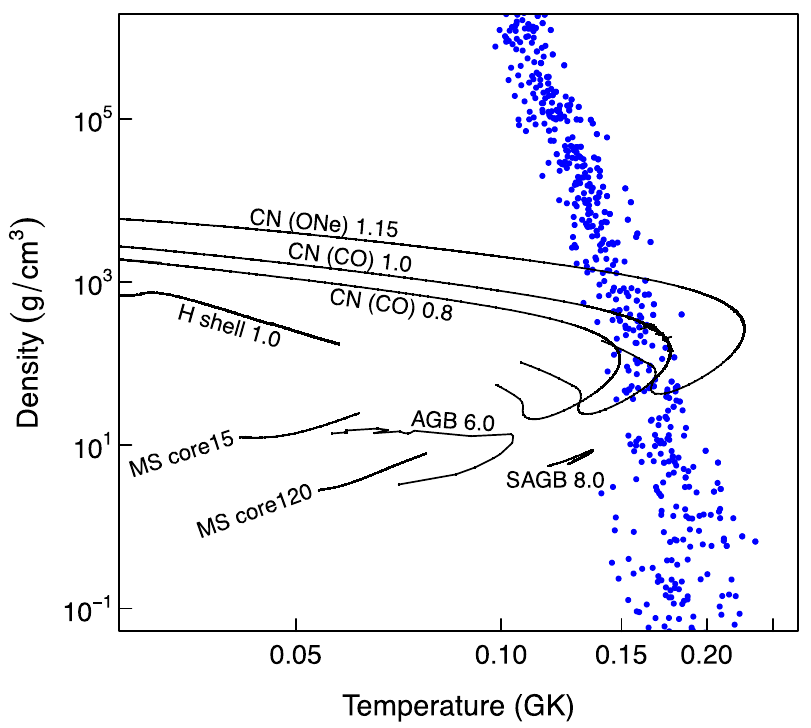
\includegraphics[width=4.5in]{Chapter-6/figs/Trho_Iliadis2016.png}
\caption{\label{fig:Trho_Iliadis}Temperature-density conditions reproducing the Mg--K anticorrelation and other abundance patterns in NGC 2419, obtained by sampling $T$, $\rho$, $X_{\mathrm{H}}$, reaction rate probability densities, and initial abundances from a nuclear reaction network (see text). The $T$--$\rho$ conditions for several polluter star candidates are represented by the black lines. Adapted from Ref. \cite{Iliadis2016}.}
\end{figure}

Ref. \cite{Iliadis2016} expanded the search for polluter candidates by performing a Monte Carlo nuclear reaction network calculation that reproduced all of the observed abundances in NGC 2419, including the Mg--K anticorrelation. The parameters that were randomly sampled include the temperature $T$, density $\rho$, final hydrogen mass fraction $X_{\mathrm{H}}$, all reaction rate probability densities in the network, and initial abundances. The reaction rates were obtained by truncating the Starlib \cite{Sallaska2013} library for the relevant rates. The resulting $T$--$\rho$ conditions that matched all of the observed abundances are shown by the blue dots in Fig. \ref{fig:Trho_Iliadis}. A narrow band of possible $T$--$\rho$ conditions was found between $\approx80-260$ MK and $\approx10^{-4}-10^{8}$ $\mathrm{g/cm}^{3}$, with additional solutions not shown in Fig. \ref{fig:Trho_Iliadis} up to $10^{11}$ $\mathrm{g/cm}^{3}$. The black bands in the figure represent the $T$--$\rho$ hydrogen burning conditions of several polluter star candidates. These include the cores of 15 $\mathrm{M}_{\odot}$ and 120 $\mathrm{M}_{\odot}$ main sequence (MS) stars, the hydrogen-burning (H) shell of a 1 $\mathrm{M}_{\odot}$ red giant star, hot-bottom burning of a 6 $\mathrm{M}_{\odot}$ and 8 $\mathrm{M}_{\odot}$ thermally-pulsing AGB and SAGB star, respectively, a 1.15 $\mathrm{M}_{\odot}$ ONe classical nova, and 0.8 $\mathrm{M}_{\odot}$ and 1.0 $\mathrm{M}_{\odot}$ CO classical novae. The only candidates that nominally overlap with this band are ONe and CO classical novae. However, another candidate Ref. \cite{Iliadis2016} considers is SAGB stars because of the large uncertainty in AGB stellar model parameters, such as the mass loss rate and the prescription of convective mixing. Adjusting these parameters within their current uncertainties could increase the temperature of HBB enough to match the observed abundances.

% PARAGRAPH 5: Dermigny et al. (2017) reaction rate sensitivities suggesting 4 reactions are important

\begin{figure}[t]
\centering
\noindent
\begin{tikzpicture}[scale=1.3, every node/.style={transform shape}]
\node at (0,0) {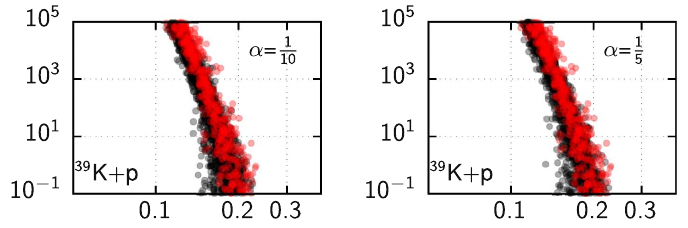
\includegraphics[scale=0.45]{Chapter-6/figs/39K_p_g_Sens1.png}};
\node at (0.04,-3.7) {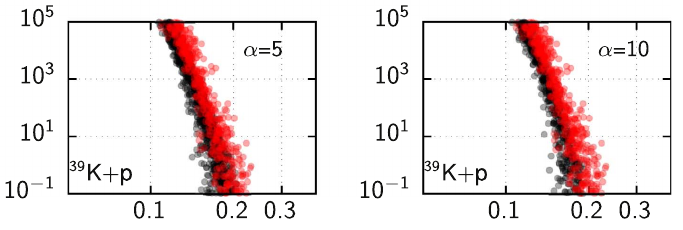
\includegraphics[scale=0.45]{Chapter-6/figs/39K_p_g_Sens2.png}};

\node at (0.3,-5.9) {Temperature (GK)};
\node[rotate=90] at (-5.7,-1.85) {Density ($\mathrm{g}/\mathrm{cm}^{3}$)};

\end{tikzpicture}
\caption{\label{fig:39K_p_g_Sens}Systematic effects of the $^{39}\mathrm{K}(p,\gamma)^{40}\mathrm{Ca}$ reaction rate influencing temperature-density conditions. The indicated variation factors ($\alpha = 1/10, 1/5, 5, 10$) are applied to the reaction rate in each panel, and the black dots show the resulting temperature-density conditions that provide an acceptable match with observed abundances. The red dots represent the case where no systematic effects ($\alpha=1$) have been added. Figure adapted from \cite{Dermigny2017}.}
\end{figure}

While Ref. \cite{Iliadis2016} simultaneously sampled the reaction rate probability densities of all the reactions in the network, they did not investigate the effect of individual reaction rates. Ref. \cite{Dermigny2017} investigated the sensitivity of the acceptable $T$--$\rho$ conditions for NGC 2419 polluter stars on unknown systematic effects of individual reaction rates. Only 4 reactions were found to make a significant impact on the acceptable $T$--$\rho$ conditions, $^{30}\mathrm{Si}(p,\gamma)^{31}\mathrm{P}$, $^{37}\mathrm{Ar}(p,\gamma)^{38}\mathrm{K}$, $^{38}\mathrm{Ar}(p,\gamma)^{39}\mathrm{K}$, and $^{39}\mathrm{K}(p,\gamma)^{40}\mathrm{Ca}$. If the reaction rate of $^{39}\mathrm{K}(p,\gamma)^{40}\mathrm{Ca}$, for example, were systematically larger than its recommended rate, by even as little as a factor of 5, the acceptable $T$--$\rho$ band would have significantly reduced scatter and would be constrained to the low-temperature side for all densities. This scenario is shown in Fig. \ref{fig:39K_p_g_Sens} on the bottom-left panel, where the black dots represent the new rate multiplied by the indicated variation factor $\alpha$, and the red dots represent the recommended rate ($\alpha = 1$). This makes sense in theory because potassium abundance would be reduced if the rate of its primary destruction reaction were increased. The high temperature conditions would therefore destroy too much potassium compared to its observed abundance. In contrast, if the rate were systematically smaller by a factor of 5, the solutions interestingly only have increased scatter. These same effects are also true for $^{30}\mathrm{Si}(p,\gamma)^{31}\mathrm{P}$, but the opposite is true for $^{37}\mathrm{Ar}(p,\gamma)^{38}\mathrm{K}$ and $^{38}\mathrm{Ar}(p,\gamma)^{39}\mathrm{K}$, as these latter reactions increase the potassium abundance.

%%%%%%%%%%%%%%%%%%%%%%%%%%%%%%%%%%%%%%%%%%%%%%%%%%%%%%%%%%%%%%%%%%%%%%%%%%%%%%%%%%%%%%%%%%%%%
\section{The Previous $^{39}\mathrm{\textbf{K}}(p,\gamma)^{40}\mathrm{\textbf{Ca}}$ Reaction Rate} \label{sec:prev_39K_p_g_rate}

The remainder of this chapter will focus specifically on the key potassium-destroying reaction $^{39}\mathrm{K}(p,\gamma)^{40}\mathrm{Ca}$, found by Ref. \cite{Dermigny2017} to be one of the few important reactions able to constrain the potassium abundance in NGC 2419 and therefore constrain the possible $T$--$\rho$ conditions of its polluter stars. 

\subsection{Longland \emph{et al.} (2018) Evaluation}

The most recent $^{39}\mathrm{K}(p,\gamma)^{40}\mathrm{Ca}$ reaction rate evaluation is that of Ref. \cite{Longland2018}, which Ref. \cite{Dermigny2017} used while it was in preparation. Its probability density was calculated using a Monte Carlo reaction rate formalism \cite{Longland2010a} with resonance strengths and resonance energies provided by the direct measurements of Refs. \cite{Kikstra1990,Cheng1981,Leenhouts1966}. The lowest directly measured resonance strength from these experiments is for the resonance at $E^{\mathrm{c.m.}}_{r} = 606$ keV. For resonances below this, indirect $^{39}\mathrm{K}(^{3}\mathrm{He},d)^{40}\mathrm{Ca}$ \cite{Cage1971} and $^{39}\mathrm{K}(d,n)^{40}\mathrm{Ca}$ \cite{Fuchs1969} proton-transfer measurements provided proton partial-widths, when available. Additionally, the indirect $^{36}\mathrm{Ar}(^{6}\mathrm{Li},d)^{40}\mathrm{Ca}$ $\alpha$-transfer measurement of Ref. \cite{Yamaya1994} provided $\alpha$-particle partial widths for the $(p,\alpha)$ channel, when available. Otherwise, measured or theoretical upper limits were given to the single particle reduced widths of the remaining resonances. These upper limits are described by the Porter-Thomas distribution \cite{Porter1956,Weidenmuller2009}, truncated at the upper limit value in the case of measured upper limits. This provided a physically motivated probability density from which to sample unknown or upper-limit partial widths.

The reaction rate probability density evaulated by Ref. \cite{Longland2018} is shown in Fig. \ref{fig:39K_p_g_Longland}. The reaction rate uncertainty is represented on the $y$-axis as a factor of the mean, recommended rate, which has been normalized to unity. The 68$\%$ (1$\sigma$) and 95$\%$ (2$\sigma$) uncertainty bands are represented by the thick and thin black lines, respectively, while the color scale indicates the continuity of the probability density. Clearly, the rate uncertainty is very large between about $0.05-0.2$ GK ($50-200$ MK), where the total $1\sigma$ width peaks at a factor of 84 at about 80 MK. Recall from Section \ref{sec:NGC2419} that the astrophysically relevant temperature range spanning the $T$--$\rho$ band in Figs. \ref{fig:Trho_Iliadis} and \ref{fig:39K_p_g_Sens} is $\approx80-260$ MK. The most recent $^{39}\mathrm{K}(p,\gamma)^{40}\mathrm{Ca}$ reaction rate is therefore very uncertain in the astrophysical temperature range of interest. This is concerning, given that Ref. \cite{Dermigny2017} found that the $T$--$\rho$ conditions are sensitive to systematic variations in the $^{39}\mathrm{K}(p,\gamma)^{40}\mathrm{Ca}$ rate, by even as little as a factor of 5. This motivates the necessity of constraining the $^{39}\mathrm{K}(p,\gamma)^{40}\mathrm{Ca}$ rate, particularly for the contributing resonances between $\approx50-260$ MK.

\begin{figure}[t]
\centering
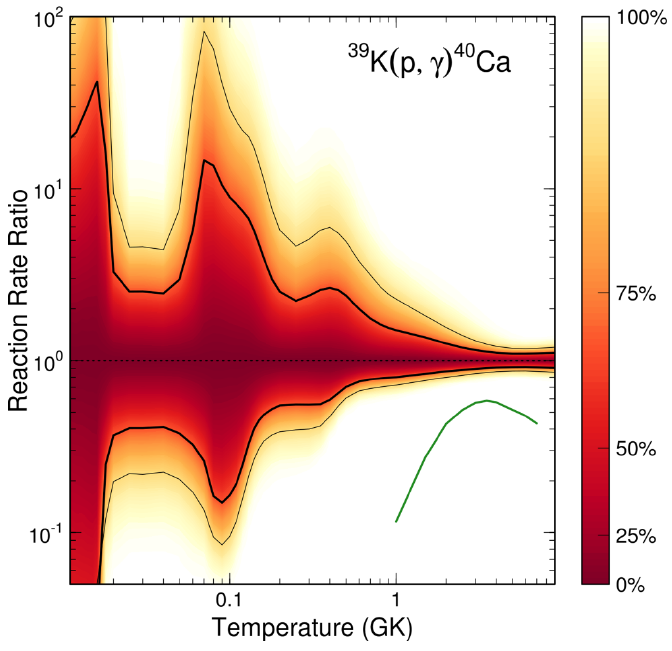
\includegraphics[width=4in]{Chapter-6/figs/39K_p_g_Longland2018.png}
\caption{\label{fig:39K_p_g_Longland}The recent $^{39}\mathrm{K}(p,\gamma)^{40}\mathrm{Ca}$ reaction rate probability density calculation of \cite{Longland2018} as a function of temperature. The median, recommended rate is shown as the dotted normalization line. The thick and thin black lines represent the $68\%$ ($1\sigma$) and $95\%$ ($2\sigma$) uncertainty bands, respectively. The color scale shows the continuous nature of the probability density, with darker red colors closer to the recommended rate. The green line represents the previous calculation of Ref \cite{Cheng1981}.}
\end{figure}

\subsection{Contributing Resonances}

Those contributing $^{39}\mathrm{K}+p$ resonances in the $\approx50-260$ MK range span resonance energies of $E^{\mathrm{c.m.}}_{r} \approx 65-560$ keV (See Section \ref{sec:Gamow}) and $^{40}$Ca excited state energies of about $E_{x} \approx 8400-8900$ keV, where the most recent $^{40}\mathrm{Ca}$ proton separation energy measurement is $S_{p} = 8328.18(2)$ keV from Ref. \cite{Wang2021}. This resonance energy range is below the lowest directly measured resonance at $E^{\mathrm{c.m.}}_{r} = 606$ keV ($E_{x} = 8935$ keV), indicating that this region is entirely described by inferred transfer reaction partial widths or upper limits at present.

\begin{figure}
\centering
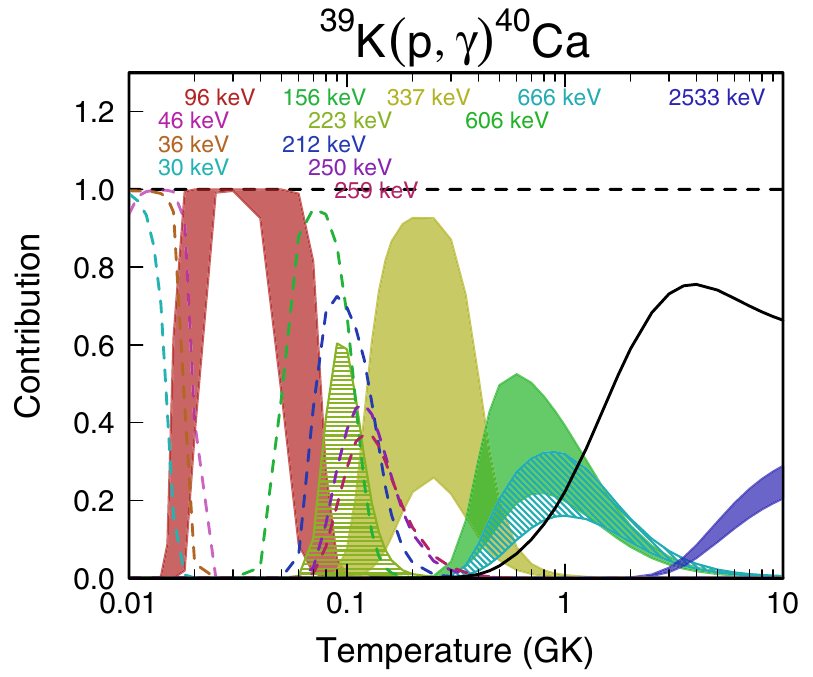
\includegraphics[width=5in]{Chapter-6/figs/Contrib_Longland2018.png}
\caption{\label{fig:contrib_longland2018}The individual resonance contributions to the $^{39}\mathrm{K}(p,\gamma)^{40}\mathrm{Ca}$ reaction rate from Ref. \cite{Longland2018} as a fraction of unity. Measured resonances are represented with shading or hatched lines and are shown with their $1\sigma$ uncertainty bands. Resonances from upper limits are represented by dashed lines and show their 84$\%$ (+$1\sigma$) value. The black line represents the total resonance contribution of all resonances that individually contribute less than $20\%$ to the total reaction rate.}
\end{figure}

The contributing resonances from the reaction rate evaluation of Ref. \cite{Longland2018} are shown in Fig. \ref{fig:contrib_longland2018}. The individual, fractional resonance contribution for each resonance is shown as a function of temperature. Measured resonances are shown with their $1\sigma$ width, representative of the Monte Carlo formalism \cite{Longland2010a} and are shaded or have hatched lines for clarity. Upper limit resonances are represented by dashed lines at their $84\%$ (+$1\sigma$) value. All resonances that individually contribute at least $20\%$ to the total reaction rate are shown in the figure with corresponding resonance energy labels, while the remaining resonance contributions sum to the black line. Of note are the 96 keV, 156 keV, and 337 keV resonances, which overwhelmingly contribute to the reaction rate at their respective temperatures. The 337 keV resonance, in particular, is the most important resonance between $\approx 0.15-0.4$ GK ($150-400$ MK), which makes up most of the astrophysical temperature range of interest, $80-260$ MK. However, the discrepancy between the $84\%$ ($+1\sigma$) contribution and the $16\%$ (-$1\sigma$) contribution is very large. The large uncertainty in the reaction rate around $50-200$ MK in Fig. \ref{fig:39K_p_g_Longland} is partly due to the uncertainty in this resonance contribution, but it is mostly a result of the many unknown resonances with only upper limit values between the 96 keV resonance and the 337 keV resonance.

%\section{The Previous $^{39}\mathrm{\textbf{K}}(^{3}\mathrm{\textbf{He}},d)^{40}\mathrm{\textbf{Ca}}$ and $^{39}\mathrm{\textbf{K}}(d,n)^{40}\mathrm{\textbf{Ca}}$ Measurements}

\subsection{Previous Proton-Transfer Measurements}

The previous $^{39}\mathrm{K}(^{3}\mathrm{He},d)^{40}\mathrm{Ca}$ \cite{Erskine1966,Seth1967,Forster1970,Cage1971} and $^{39}\mathrm{K}(d,n)^{40}\mathrm{Ca}$ \cite{Fuchs1969} proton-transfer measurements were not capable of achieving high resolution, particularly for unbound $^{40}$Ca states, i.e. at energies above the proton separation energy. The ($^{3}\mathrm{He},d$) measurements of Refs. \cite{Erskine1966,Seth1967,Cage1971} obtained spectroscopic factors ($C^{2}S$) for only 2 unbound $^{40}$Ca states, with ENSDF \cite{Chen2017} excitation energies of $E_{x} = 8425$ keV ($E^{\mathrm{c.m.}}_{r} = 96$ keV) and 8551 keV ($E^{\mathrm{c.m.}}_{r} = 223$ keV), which are both below the lowest directly measured resonance at $E_{x} = 8935$ ($E^{\mathrm{c.m.}}_{r} = 606$ keV). Meanwhile, Ref. \cite{Forster1970} did not observe unbound $^{40}$Ca states due to their focus on lower energy excited states. The $(d,n)$ measurement of Ref. \cite{Fuchs1969} obtained $C^{2}S$ for 14 unbound $^{40}$Ca states, with only 4 of these states below the lowest directly measured resonance, including $8359$ keV ($E^{\mathrm{c.m.}}_{r} = 30$ keV), $8425$ keV ($E^{\mathrm{c.m.}}_{r} = 96$ keV), $8551$ keV ($E^{\mathrm{c.m.}}_{r} = 223$ keV), and $8665$ keV ($E^{\mathrm{c.m.}}_{r} = 337$ keV). Hence, there is an overlap between the $(^{3}\mathrm{He},d)$ and $(d,n)$ measurements of 2 unbound $^{40}$Ca states, 8425 keV ($E^{\mathrm{c.m.}}_{r} = 96$ keV) and 8551 keV ($E^{\mathrm{c.m.}}_{r} = 223$ keV). The $^{39}\mathrm{K}(p,\gamma)^{40}\mathrm{Ca}$ reaction rate calculation of Ref. \cite{Longland2018} used the $C^{2}S$ measurements of Ref. \cite{Cage1971} for these 2 states, due to their more sophisticated coupled-channel DWBA calculations. They used the $C^{2}S$ measurement of Ref. \cite{Fuchs1969} for the 8665 keV ($E^{\mathrm{c.m.}}_{r} = 337$ keV) state. However, the reaction rate calculation did not include the 8359 keV ($E^{\mathrm{c.m.}}_{r} = 30$ keV) $C^{2}S$ measurement of Ref. \cite{Fuchs1969}, as this state has an energy discrepancy with ENSDF \cite{Chen2017} of 12 keV. This resonance was instead given an upper limit. Several unknown resonances remain below $E_{x} = 8935$ keV ($E^{\mathrm{c.m.}}_{r} = 606$ keV). Ref. \cite{Longland2018} uses upper limits for 18 resonances in this region. Hence, this was strong motivation to revisit the proton-transfer reaction at modern resolution to potentially resolve the currently unknown resonances.

%%%%%%%%%%%%%%%%%%%%%%%%%%%%%%%%%%%%%%%%%%%%%%%%%%%%%%%%%%%%%%%%%%%%%%%%%%%%%%%%%%%%%%%%%%%%%
\section{The $^{39}\mathrm{\textbf{K}}(^{3}\mathrm{\textbf{He}},d)^{40}\mathrm{\textbf{Ca}}$ Experiment}

% PARAGRAPH 1: Basically like the methods section in my 39K(3He,d)40Ca PRL paper, but go into much more detail about the tandem, enge, and detector setup. Note: I will have already covered these in detail in Ch 4
% PARAGRAPH 2: Show an example spectrum with peaks labeled
% PARAGRAPH 3: Different spectra from the FP and Si detectors, including DE/E for particle discrimination.

The $^{39}\mathrm{K}(^{3}\mathrm{He}, d)^{40}\mathrm{Ca}$ experiment was performed in 2019 over 5 days using the Enge Split-Pole Spectrograph at the Triangle Universities Nuclear Laboratory (TUNL). The 10 MV FN tandem Van de Graaff accelerator at TUNL accelerated a fully-ionized $^{3}$He beam to  $E_{\mathrm{lab}} = 21$ MeV, where the energy was stabilized using a pair of high-resolution slits between two $90^{\circ}$ dipole magnets (see Section \ref{sec:exp} for experimental details). The $^{39}\mathrm{K}(^{3}\mathrm{He},d)^{40}\mathrm{Ca}$ proton transfer and $^{39}\mathrm{K}(^{3}\mathrm{He},^{3}\mathrm{He})^{39}\mathrm{K}$ elastic scattering reactions were measured separately between $\theta_{\mathrm{lab}} = 5-20^{\circ}$ and $ \theta_{\mathrm{lab}} = 15-59^{\circ}$, respectively, using the focal plane detector package of Ref. \cite{Marshall2019}. The $d$ and $^{3}$He particles that were ejected from the target at the angle $\theta_{\mathrm{lab}}$ passed through the magnetic field $B$ of the Enge Split-Pole Spectrograph, where they were then focused at a position along the focal plane, based on their magnetic rigidity $B\rho$ (See Sec. \ref{sec:Brho}). The focal-plane detector was preemptively moved via dual motors to align itself with the focal plane. Meanwhile, for every $^{39}\mathrm{K}(^{3}\mathrm{He},d)^{40}\mathrm{Ca}$ or $^{39}\mathrm{K}(^{3}\mathrm{He},^{3}\mathrm{He})^{39}\mathrm{K}$ focal-plane measurement, the $^{39}\mathrm{K}(^{3}\mathrm{He},^{3}\mathrm{He})^{39}\mathrm{K}$ reaction was simultanesouly measured with a silicon detector telescope inside the target chamber, positioned at a constant $45^{\circ}$ from the beamline to monitor potential target degradation and other target properties.

\subsection{Targets}

A total of 7 natural KI ($93.26\%$ $^{39}$K, $6.73\%$ $^{41}$K) targets were made throughout the course of the experiment, in 2 separate evaporation batches (see Section \ref{sec:Evap} for details on the evaporation procedure). The targets labeled KI $\#$1, KI $\#$2, and KI $\#$3 were made in the first batch, while those labeled KI $\#$4, KI $\#$5, KI $\#$6, and KI $\#$7 were made in the second batch, on the second day of the experiment. For each batch, the targets were simultaneously produced by evaporating approximately 75 $\mu\mathrm{g/cm}^{2}$ of natural KI onto aluminum target frames, each with a 21 $\mu\mathrm{g/cm}^{2}$ natural carbon ($98.84\%$ $^{12}$C, $0.96\%$ $^{13}$C) foil backing. The KI target thickness was measured by a thickness monitor inside the evaporation chamber, placed at roughly the same distance from the evaportion material as were the aluminum target frames with carbon backings.
%Fig. \ref{fig:KI_Evap} shows a photograph of the chamber just before the evaporation process, with 3 natural carbon targets in position. 
A separate 21 $\mu\mathrm{g/cm}^{2}$ natural carbon target was also used in the experiment for calibrations with the $^{12}\mathrm{C}(^{3}\mathrm{He},d)^{13}\mathrm{N}$, $^{13}\mathrm{C}(^{3}\mathrm{He},d)^{14}\mathrm{N}$, and $^{16}\mathrm{O}(^{3}\mathrm{He},d)^{17}\mathrm{F}$ reactions, among other contaminants.

%\begin{figure}[t]
%\centering
%\begin{tikzpicture}[scale=1.0, every node/.style={transform shape}]
%\node[rotate=270] at (0,0) {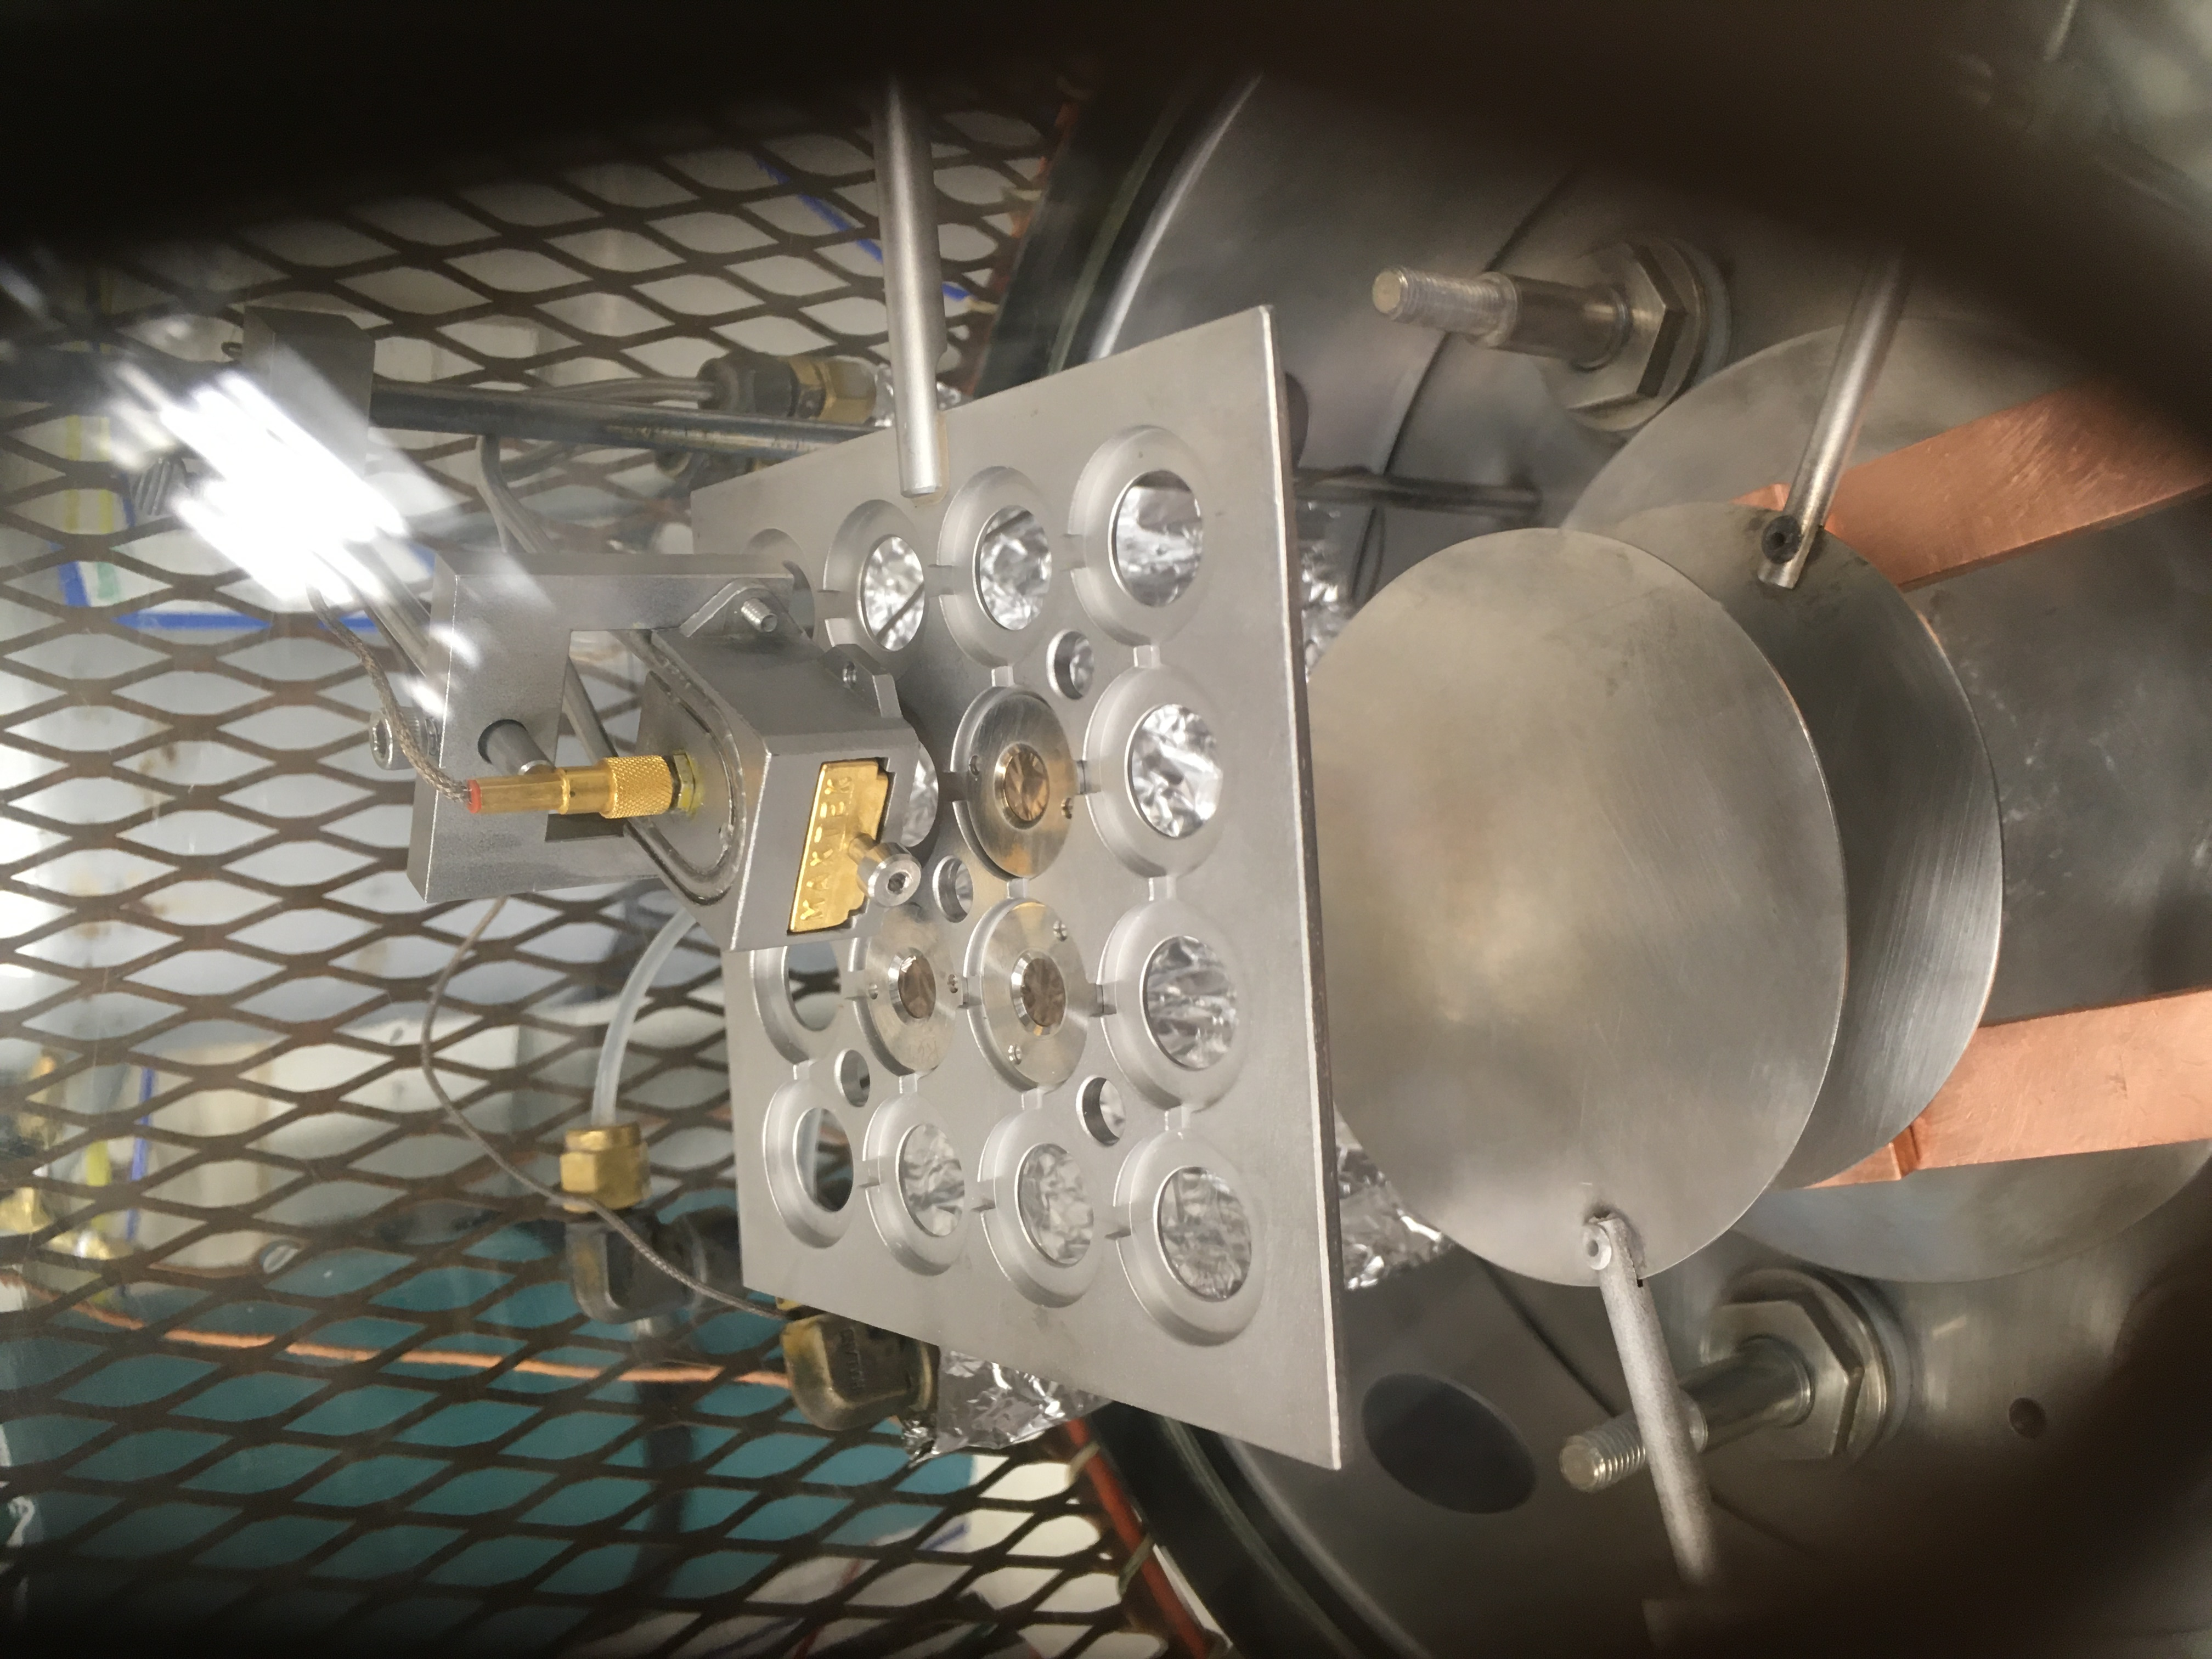
\includegraphics[width=5.4in]{Chapter-6/figs/KI_Evap.jpg}};
%\end{tikzpicture}
%\caption{\label{fig:KI_Evap}The evaporation chamber before the production of KI targets. The 3 targets shown in position become the KI $\#$1, KI $\#$2, and KI $\#$3 targets after evaporation. The thickness monitor is also shown in position around a fourth opening in the 16-slot target holder.}
%\end{figure}

Potassium iodide is hygroscopic, meaning it will eventually oxidize at atmospheric pressure. To prevent this, care was taken to transport the targets from the evaporation chamber to the target chamber in a vacuum-sealed box at rough vacuum ($\sim 10^{-2}$ torr), where they were then exposed to high vacuum ($\sim 10^{-6}$ torr) for the remainder of the experiment. However, as will be described later, the first batch of targets (KI $\#$1, KI $\#$2, and KI $\#$3) oxidized at some point during the first day of the experiment, for the $\theta_{\mathrm{lab}} = 5^{\circ}$ and $7^{\circ}$ ($^{3}\mathrm{He},d$) measurements. The focal-plane spectra for these runs, exclusively using the KI $\#$1 target, consisted of peaks with high-energy tails, expected of targets that undergo oxidation \cite{Landau1944}. These angles were measured again toward the end of the experiment with the non-oxidized KI $\#$6 target, but the oxidized KI $\#$1 data was not discarded nevertheless. Section \ref{subsec:oxidation} details a novel technique for fitting these spectra, an example of which is shown in Section \ref{subsec:oxidized_spectra}.

\subsection{Focal-Plane Spectra}

\def\yTS{1.29} % y tick space
\def\xTS{2.165} % x tick space

\begin{figure}[t]
\centering
\begin{tikzpicture}[scale=1.0, every node/.style={transform shape}]
\node at (0,0) {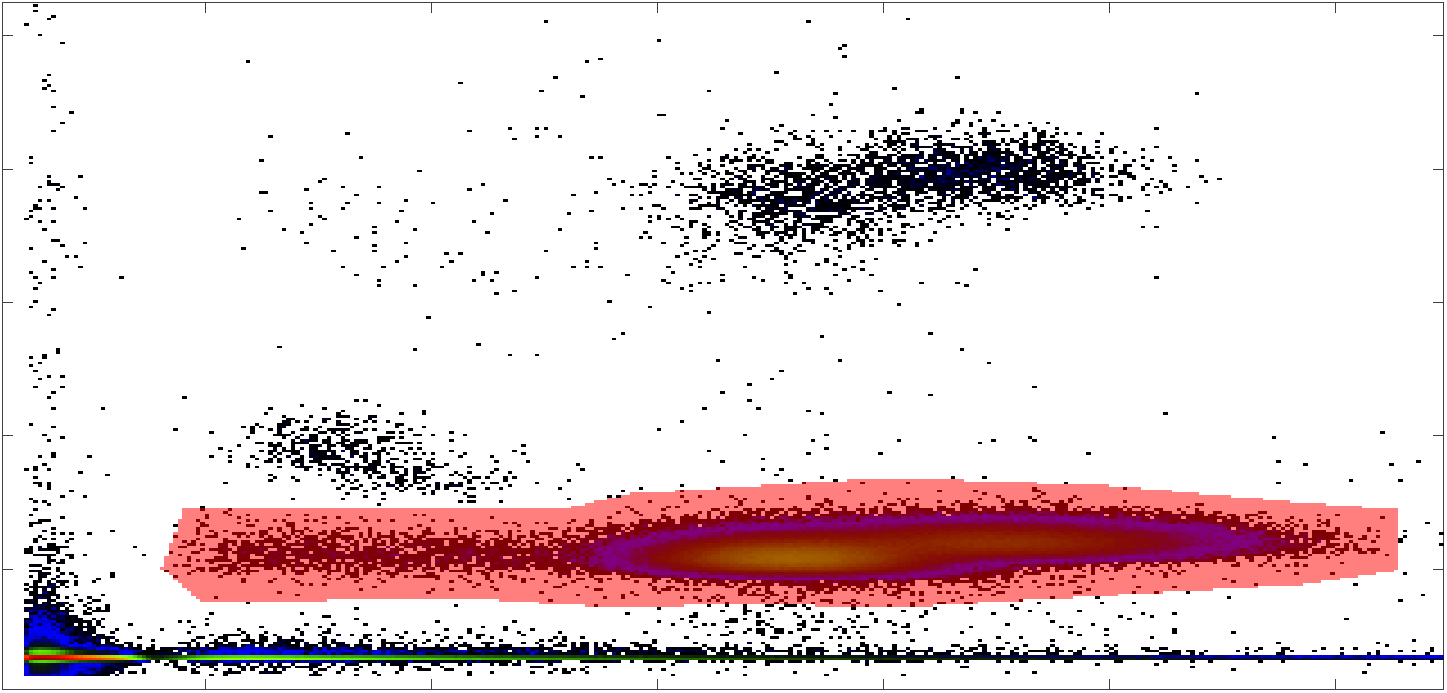
\includegraphics[width=5.5in]{Chapter-6/figs/5deg_DEvsE.png}};
\node at (-8.0,-2) {\rlap{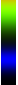
\includegraphics[scale=0.6]{Chapter-6/figs/5deg_DEvsE_Scale.png}}};

\node[rotate=90] at (-8.0,0) {$\Delta$E};
\node at (0,-3.95) {E};

\node at (-7.4,-2.15) {\rlap{\footnotesize{50}}};
\node at (-7.55,-2.15+\yTS) {\rlap{\footnotesize{100}}};
\node at (-7.55,{-2.15+(2*\yTS)}) {\rlap{\footnotesize{150}}};
\node at (-7.55,{-2.15+(3*\yTS)}) {\rlap{\footnotesize{200}}};
\node at (-7.55,{-2.15+(4*\yTS)}) {\rlap{\footnotesize{250}}};

\node at (-5.2,-3.55) {\rlap{\footnotesize{50}}};
\node at (-5.2+\xTS,-3.55) {\rlap{\footnotesize{100}}};
\node at ({-5.2+(2*\xTS)},-3.55) {\rlap{\footnotesize{150}}};
\node at ({-5.2+(3*\xTS)},-3.55) {\rlap{\footnotesize{200}}};
\node at ({-5.2+(4*\xTS)},-3.55) {\rlap{\footnotesize{250}}};
\node at ({-5.2+(5*\xTS)},-3.55) {\rlap{\footnotesize{300}}};

\node at (-8.65,-1.35) {\rlap{\scriptsize{1296}}};
\node at (-8.5,-1.62) {\rlap{\scriptsize{216}}};
\node at (-8.35,-1.92) {\rlap{\scriptsize{36}}};
\node at (-8.20,-2.22) {\rlap{\scriptsize{6}}};
\node at (-8.20,-2.52) {\rlap{\scriptsize{1}}};
\node at (-8.20,-2.82) {\rlap{\scriptsize{0}}};

\node at (1,-0.8) {\rlap{\LARGE{$\textbf{d}$}}};
\node at (-3.5,-0.1) {\rlap{\LARGE{$\textbf{t}$}}};
\node at (1.9,0.65) {\rlap{\LARGE{$^{\textbf{3}}$\textbf{He}}}};

\end{tikzpicture}
\caption{\label{fig:5deg_DEvsE}A 2D histogram of the focal-plane $\Delta$E vs E detector signals. Different groups correspond to different particles depending on their mass and charge. The deuteron group, highlighted in red, is being gated on in the figure.}
\end{figure}

The focal-plane detector package (see Section \ref{sec:fp} and Ref. \cite{Marshall2019}) consists of two position-sensitive avalanche counters, one located in the front of the detector (P1 section) and one located near the back (P2 section), a gas proportionality counter ($\Delta\mathrm{E}$ section), and a residual energy scintillator (E section). The data acquisition system (DAQ) triggers on the E section, located at the back of the detector, so that coincidences with all sections are established (see Section \ref{sec:DAQ}). The combination of the $\Delta$E and E sections enables particle discrimination based on mass and charge, allowing a given particle to be gated on and therefore filtering out undesired particles and detector noise in other spectra. In the $^{39}\mathrm{K}(^{3}\mathrm{He},d)^{40}\mathrm{Ca}$ experiment, the $\Delta\mathrm{E}/\mathrm{E}$ spectrum was used to gate on the deuteron group for $^{39}\mathrm{K}(^{3}\mathrm{He},d)^{40}\mathrm{Ca}$ and the $^{3}\mathrm{He}$ group for $^{39}\mathrm{K}(^{3}\mathrm{He},^{3}\mathrm{He})^{39}\mathrm{K}$. Figure \ref{fig:5deg_DEvsE} shows an example 2D histogram of $\Delta$E vs E in the offline \texttt{Jam} software package \cite{Swartz2001,Jam} for the KI $\#$6 target at $\theta_{\mathrm{lab}} = 5^{\circ}$ and an Enge magnetic field of $B = 1.14$ T. The $d$, $t$, and $^{3}$He particles appear in groups, with the $d$ group highlighted in red to represent a gate. The $p$ group is joined by noise in the $\Delta$E detector below the $\Delta$E threshold and are filtered out along with the other particle groups. Both the $\Delta$E and E signals are compressed from their original 4096 channels to 512 channels in the 2D spectrum. 

The 1D histogram of the P1 section, gated on the deuteron group of Fig \ref{fig:5deg_DEvsE}, is shown in Fig. \ref{fig:5deg_fp} in red. The overlayed black spectrum is from a carbon target to show overlapping peaks, indicating contaminants in the KI target. The deuteron peaks shown only in red were ejected from $^{39}\mathrm{K}(^{3}\mathrm{He},d)^{40}\mathrm{Ca}$ reactions in the KI target, where different excited states of the $^{40}$Ca recoil nuclei were populated, resulting in different kinematics for each deuteron depending on the excited state. High-energy deuterons are associated with high-energy $^{40}$Ca excited states, and vice versa. The deuterons are momentum-separated by the Enge Split-Pole Spectrograph, focusing the higher energy ones on the left side of the position sections and the lower energy ones on the right side. Thus, the P1 channel number in Fig. \ref{fig:5deg_fp} is inversely related to the $^{40}$Ca excited state energies. The same is true of the excited states from the contaminants.

\def\yTS{0.72}
\def\xTS{2.12}

\begin{figure}[t]
\centering
\begin{tikzpicture}[scale=1.0, every node/.style={transform shape}]
\node[rotate=90] at (-8.50,0) {P1 Counts};
\node at (0,-3.6) {Channel};
\node at (0,0) {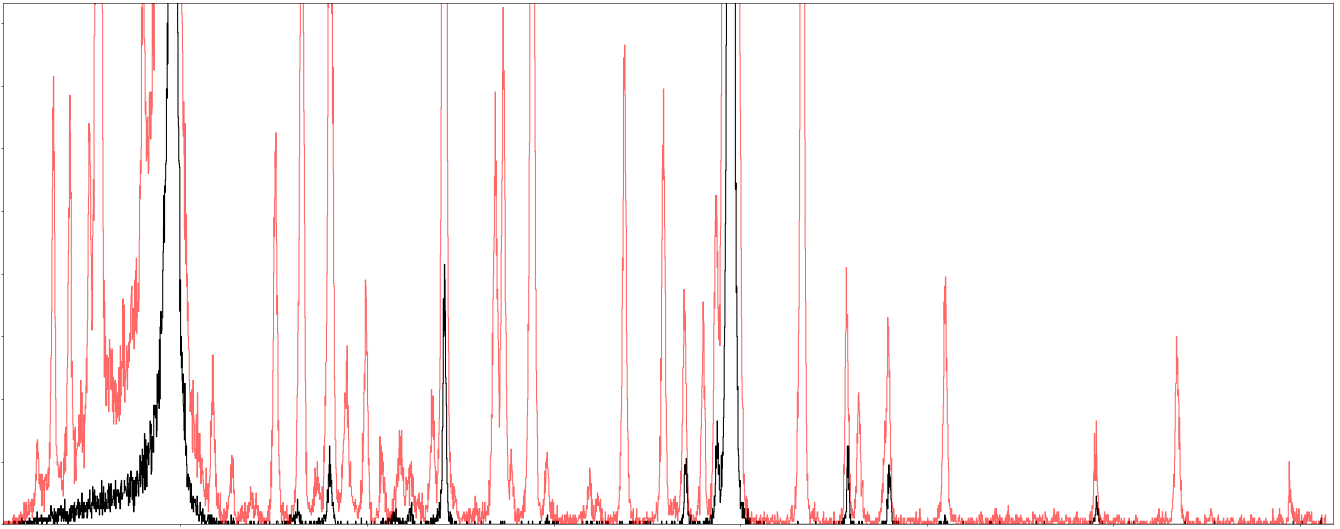
\includegraphics[width=6in]{Chapter-6/figs/5deg_KI6.png}};
\node at (-7.85,-3.0) {\rlap{\footnotesize{0}}};
\node at (-8.00,-3.0+\yTS) {\rlap{\footnotesize{20}}};
\node at (-8.00,{-3.0+(2*\yTS)}) {\rlap{\footnotesize{40}}};
\node at (-8.00,{-3.0+(3*\yTS)}) {\rlap{\footnotesize{60}}};
\node at (-8.00,{-3.0+(4*\yTS)}) {\rlap{\footnotesize{80}}};
\node at (-8.20,{-3.0+(5*\yTS)}) {\rlap{\footnotesize{100}}};
\node at (-8.20,{-3.0+(6*\yTS)}) {\rlap{\footnotesize{120}}};
\node at (-8.20,{-3.0+(7*\yTS)}) {\rlap{\footnotesize{140}}};
\node at (-8.20,{-3.0+(8*\yTS)}) {\rlap{\footnotesize{160}}};

\node at (-5.95,-3.18) {\rlap{\footnotesize{1000}}};
\node at (-5.95+\xTS,-3.18) {\rlap{\footnotesize{1500}}};
\node at ({-5.95+(2*\xTS)},-3.18) {\rlap{\footnotesize{2000}}};
\node at ({-5.95+(3*\xTS)},-3.18) {\rlap{\footnotesize{2500}}};
\node at ({-5.95+(4*\xTS)},-3.18) {\rlap{\footnotesize{3000}}};
\node at ({-5.95+(5*\xTS)},-3.18) {\rlap{\footnotesize{3500}}};
\node at ({-5.95+(6*\xTS)},-3.18) {\rlap{\footnotesize{4000}}};
\end{tikzpicture}
\caption{\label{fig:5deg_fp}A histogram spectrum of the front (P1) focal-plane detector position section at $\theta_{\mathrm{lab}} = 5^{\circ}$ and $E_{\mathrm{lab}} = 21$ MeV with the KI $\#$6 target (in red) and the carbon target (in black), both gated on the deuteron group from the the $\Delta$E vs. E spectrum. Overlapping peaks indicate contaminants.}
\end{figure}

\subsection{Energy Shifts} \label{subsec:energy_shifts}

% I want to cover all the angles, targets, magnetic fields, and sort groups. Introduce what I mean by sort groups. Cover energy shifts for various reasons, the Pos1 vs Event spectrum, etc.

The P1 peak centroid positions typically remain constant over time. However, certain changes in the beam can introduce shifts in these positions, broadening the peaks over more channels than usual. For instance, adjusting the beam steerers or focusing elements at any point along the beamline can cause very slight kinematic differences to occur in the target. This is because the target material is never perfectly uniformly-distributed. Sometimes these differences in kinematics are large enough to cause a noticable drift in the P1 spectrum. Retuning the beam between runs at the same Engle angle $\theta_{\mathrm{lab}}$ is the most common example of energy shifts, followed by switching between targets from a different evaporation batch. Any unintentional beam drift can also cause them, albeit usually to a lesser degree.

To visualize these energy shifts, the P1 spectrum must be traced over time. This feature was recently added to the offline version of the \texttt{EngeSpec} \cite{EngeSpec} graphical user interface (GUI), and I implemented the same feature in my local \texttt{Jam} source code. For each event, the P1 data is collected and the event number is recorded during the sort routine. The total number of events is unknown until the end of the sort routine, which unfortunately makes an online version of this feature nearly impossible. The 4096-channel P1 data and the corresponding event numbers are compressed into 512 bins, where they each get incremented into a 2D histogram.

There were a few instances of energy shifts during the $^{39}\mathrm{K}(^{3}\mathrm{He},d)^{40}\mathrm{Ca}$ experiment. One happened due to a necessary beam-retune after a tour group was scheduled to view the tandem accelerator. The low-energy beamline Faraday cup was put in place for about an hour, and tuning was required to get the beam back on target. The runs before and after this retune are represented by the 2D histogram of P1 vs event number in Fig. \ref{fig:9deg_P1vsEvt}. Depicted in the figure are the runs $\#23-\#27$ at $\theta_{\mathrm{lab}} = 9^{\circ}$ with the KI $\#$5 target. The P1 section is zoomed in on the $^{12}$C ground state, as it had the most counts and is therefore easiest to visualize energy shifts. The $^{12}$C ground state centroid starts at P1 bin number 296, and a clear shift to bin number 297 is seen at event number 320. A 1-bin shift in the 512-bin 2D spectrum corresponds to an 8-channel shift in the 4096-channel P1 spectrum, which was noticable even during the experiment. Based on the BCI of each run, it was easy to determine that the shift happened between runs $\#$25 and $\#$26, exactly when the retune happend. This is also evident from the shift in counts at this point because more beam current was acquired as a result of the retune. There is also an unknown phenomenon just after event bin number 100, occurring during run $\#$23. The peaks do not appear to be shifted from it, at least not as dramatically as from the retune, but it is clear that the beam current changed abruptly.

\def\yTS{0.635} % y tick space
\def\xTS{2.48} % x tick space

\begin{figure}[t]
\centering
\begin{tikzpicture}[scale=1.12, every node/.style={transform shape}]
\node at (0,0) {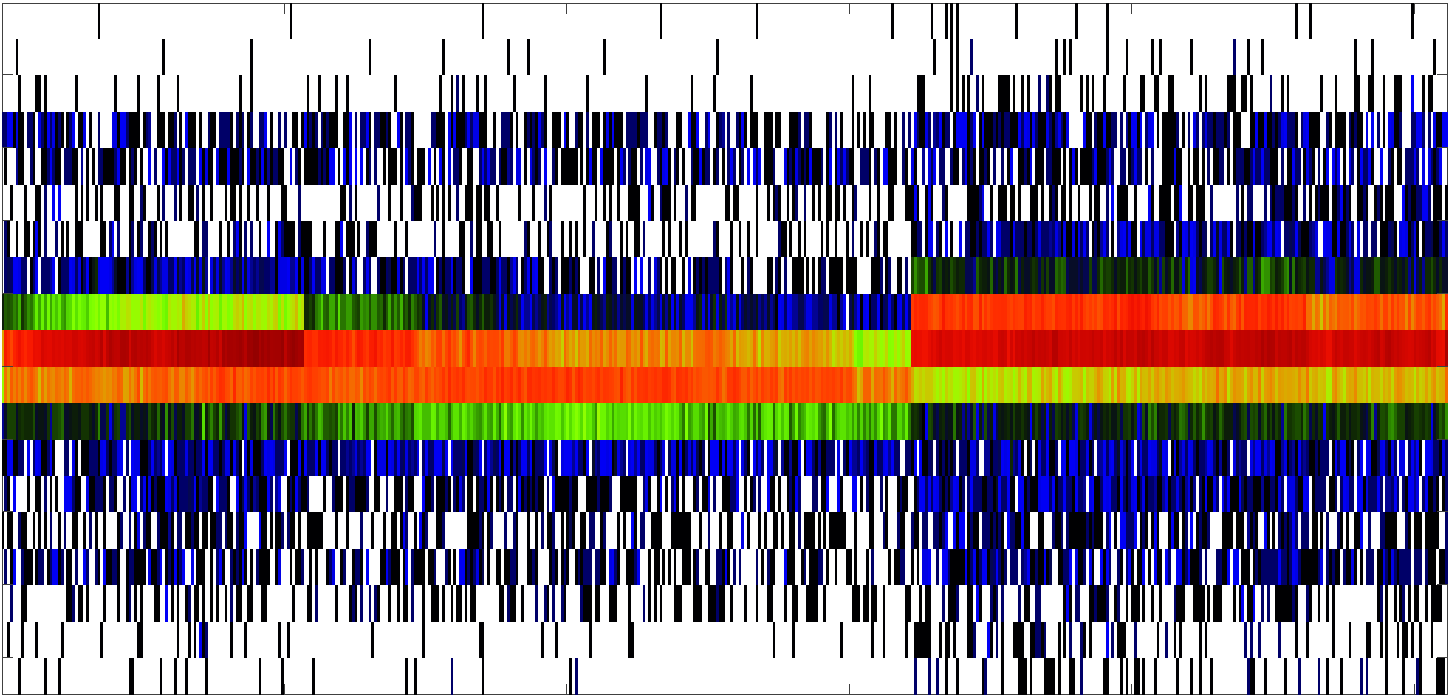
\includegraphics[width=5in]{Chapter-6/figs/9deg_AllRuns_Pos1vsEvent.png}};
\node at (0,-3.8) {Event Number};
\node[rotate=90] at (-7.5,0) {P1};
\node at (-6.7,2.4) {\footnotesize{304}};
\node at (-6.7,2.4-\yTS) {\footnotesize{302}};
\node at (-6.7,{2.4-(2*\yTS)}) {\footnotesize{300}};
\node at (-6.7,{2.4-(3*\yTS)}) {\footnotesize{298}};
\node at (-6.7,{2.4-(4*\yTS)}) {\footnotesize{296}};
\node at (-6.7,{2.4-(5*\yTS)}) {\footnotesize{294}};
\node at (-6.7,{2.4-(6*\yTS)}) {\footnotesize{292}};
\node at (-6.7,{2.4-(7*\yTS)}) {\footnotesize{290}};
\node at (-6.7,{2.4-(8*\yTS)}) {\footnotesize{288}};

\node at (-3.9,-3.3) {\footnotesize{100}};
\node at (-3.9+\xTS,-3.3) {\footnotesize{200}};
\node at ({-3.9+(2*\xTS)},-3.3) {\footnotesize{300}};
\node at ({-3.9+(3*\xTS)},-3.3) {\footnotesize{400}};
\node at ({-3.9+(4*\xTS)},-3.3) {\footnotesize{500}};
\node at (-7.72,-1.05) {\scriptsize{243}};
\node at (-7.68,-1.35) {\scriptsize{81}};
\node at (-7.68,-1.65) {\scriptsize{27}};
\node at (-7.62,-1.95) {\scriptsize{9}};
\node at (-7.62,-2.25) {\scriptsize{3}};
\node at (-7.62,-2.55) {\scriptsize{1}};
\node at (-7.62,-2.85) {\scriptsize{0}};

%\hspace{-0.2cm}
% Fix first \includegraphics figure in place, and place second figure to the bottom left (right) with \rlap (\llap). Use \rlap{\raisebox{3cm}{\include ...}} to raise the figure
\node at (-7.5,-2) {\rlap{
\includegraphics[scale=0.6]{Chapter-6/figs/9deg_Scale.png}}};

\end{tikzpicture}
\caption{\label{fig:9deg_P1vsEvt}A 2D histogram of the front (P1) focal-plane position section vs event number over all $^{39}\mathrm{K}(^{3}\mathrm{He},d)^{40}\mathrm{Ca}$ runs ($\#23-\#27$) at $\theta_{\mathrm{lab}} = 9^{\circ}$ with the KI $\#$5 target. Both axes are compressed to 512 channels. The P1 section is zoomed in on the $^{12}$C gound state to show the effect of energy shifts due to beam retunes. A beam retune after run $\#$25 caused the shift in the P1 spectrum shown at event (bin) number 320. The unknown phenomenon at event (bin) number 100 occurred during run $\#$23, which caused a reduction in counts but no energy shift.}
\end{figure}

\begin{table}[t]
\centering
\caption{\label{tab:run}Information on each run of the $^{39}\mathrm{K}(^{3}\mathrm{He}, d)^{40}\mathrm{Ca}$ experiment, including the angle of the Enge, the target used, the magnetic field of the Enge, and the sort group (see text).}
%\begin{tabularx}{\textwidth}{ccccc}
\begin{tabular}{ccccc}
\hline\midrule
Sort Group&$\theta_{\mathrm{lab}}$ $[^{\circ}]$&Run Numbers&Target&Enge Field [$T$]\\ \midrule
1&5&9, 10&KI $\#$1&1.14\\
2&5&11&KI $\#$1&1.14\\
3&5&$83-87$&KI $\#$6&1.14\\
4&7&$15-20$&KI $\#$1&1.14\\
5&7&72, $75-78$&KI $\#$6&1.14\\
6&9&23&KI $\#$5&1.145\\
7&9&24, 25&KI $\#$5&1.145\\
8&9&26, 27&KI $\#$5&1.145\\
9&11&$31-33$&KI $\#$5&1.145\\
10&13&$39-41$&KI $\#$5&1.145\\
11&13&42&KI $\#$5&1.145\\
12&13&43, 44&KI $\#$5&1.145\\
13&13&45, 47&KI $\#$5, KI $\#$6&1.145\\
14&15&$55-59$&KI $\#$6&1.145\\
15&20&60, 61, 64&KI $\#$6&1.145\\
16&20&65, 66&KI $\#$6&1.145\\
\hline\hline
%\end{tabularx}
\end{tabular}
%\footnotetext{Even though this sort group uses 2 different targets, the focal-plane peaks do not shift between them. The targets are from the same evaporation batch and therefore should have the same thickness.}
\end{table}

It would not be appropriate to sort all runs at $\theta_{\mathrm{lab}} = 9^{\circ}$ together for the $^{39}\mathrm{K}(^{3}\mathrm{He},d)^{40}\mathrm{Ca}$ energy calibration and yield analysis. Because of the presence of energy shifts at some angles, it was necessary to group runs together based on where the energy shifts occurred. I refer to these groups as \emph{sort groups}. All of the runs in the $^{39}\mathrm{K}(^{3}\mathrm{He},d)^{40}\mathrm{Ca}$ experiment, as well as their sort groups, are shown in Table \ref{tab:run}. Because there were 7 angles measured in this experiment ($\theta_{\mathrm{lab}} = 5^{\circ}, 7^{\circ}, 9^{\circ}, 11^{\circ}, 13^{\circ}, 15^{\circ}$ and $20^{\circ}$), the ideal scenario would be to have 7 sort groups, 1 for each angle. However, there are 16 sort groups for various reasons, including beam retunes, switching targets, and the occassional beam noise from beamline element power supplies failing. In the case of sort group $\#$13 at $\theta_{\mathrm{lab}} = 13^{\circ}$, consisting of runs $\#$45 and $\#$47, 2 different targets are used between them, but they are from the same evaporation batch and therefore did not cause an energy shift. The $^{39}\mathrm{K}(^{3}\mathrm{He}, {}^{3}\mathrm{He})^{39}\mathrm{K}$ P1 spectra fortunately did not contain energy shifts because only a single run was needed per angle, and the same target (KI $\#$7) was used for each run.

In the case of the $^{39}\mathrm{K}(^{3}\mathrm{He},d)^{40}\mathrm{Ca}$ run $\#$23 at $\theta_{\mathrm{lab}} = 9^{\circ}$, and for a few other runs, the energy shift occurred during the run, not between runs. For this reason, it was also necessary to have the ability to gate on the P1 vs Event Number histogram for the entire area before or after a shift. I added this feature to both my local \texttt{EngeSpec} and \texttt{Jam} source codes. Only the events occurring in the gate are used in a new, event-gated P1 spectrum. Unfortunately, this means that the recorded BCI is no longer accurate. An approximation to the new, reduced BCI is to scale the original BCI by the fraction of events in the gate. This is not exact due to the loss of resolution when compressing the events into 512 bins, but it is more than sufficient considering the much larger uncertainty from the BCI measurement itself. The same fraction can be applied to the time-keeping scalars to correct for the new deadtime. The exact same gate is also used in these cases for the simultaneous silicon detector telescope spectra, as introduced in the next section, to ensure consistency with the reduced BCI and deadtime between the focal-plane and silicon detector spectra. This is essential for a relative measurement between the two detectors, as discussed in Section \ref{subsec:SiNorm}.

\subsection{Silicon Detector Telescope} \label{subsec:SiDet}

To minimize the effects of uncertainty in the target thickness, non-uniformity in the target, and target degradation after exposure to the beam, the $^{39}\mathrm{K}(^{3}\mathrm{He}, {}^{3}\mathrm{He})^{39}\mathrm{K}$ elastic scattering and $^{39}\mathrm{K}(^{3}\mathrm{He}, d)^{40}\mathrm{Ca}$ proton-transfer yields from the focal-plane P1 spectra were normalized to the simultaneous $^{39}\mathrm{K}(^{3}\mathrm{He}, {}^{3}\mathrm{He})^{39}\mathrm{K}$ elastic scattering yield of a Si detector telescope positioned at a constant $\theta_{\mathrm{lab}} = 45^{\circ}$ inside the target chamber. The scale for the Si-normalized focal-plane differential cross-section measurements was then corrected using the global $^{3}\mathrm{He}$ optical model potential (OMP) differential cross-section for $^{39}\mathrm{K}$ from Ref. \cite{Liang2009} (see Sections \ref{subsec:SiNorm} and \ref{subsec:global_norm}). The scaling factor was the ratio between the differential cross-section of the global OMP and that of the Si-normalized focal-plane $^{39}\mathrm{K}(^{3}\mathrm{He}, {}^{3}\mathrm{He})^{39}\mathrm{K}$ measurements.

The silicon detector telescope consists of a $\Delta$E detector and a thicker, residual energy E detector, used in coincidence for particle discrimination in the same way as the $\Delta$E and E focal-plane detectors. A representative 2D $\Delta$E vs E histogram for the silicon detectors at $\theta_{\mathrm{lab}} = 45^{\circ}$ with the KI $\#$6 target is shown in Fig. \ref{fig:5deg_SiDEvsSiE}. As before, different groups correspond to different particles depending on mass and charge. The highlighted gate is around the $^{3}$He group. It is clear that there are 4 regions in this group that are more dense than the background and that have an even more negative slope than the trend of the overall group. These different regions correspond to scattering from different elements in the target. From left to right, they are carbon, oxygen, potassium, and iodine, as the more massive elements will deposit more energy in the Si E detector. 

\def\yTS{1.175} % y tick space
\def\xTS{2.165} % x tick space
\def\sl{0.28} % shift left
\def\su{0.4} % shift up

\begin{figure}[t]
\centering
\begin{tikzpicture}[scale=1.0, every node/.style={transform shape}]
\node at (0,0) {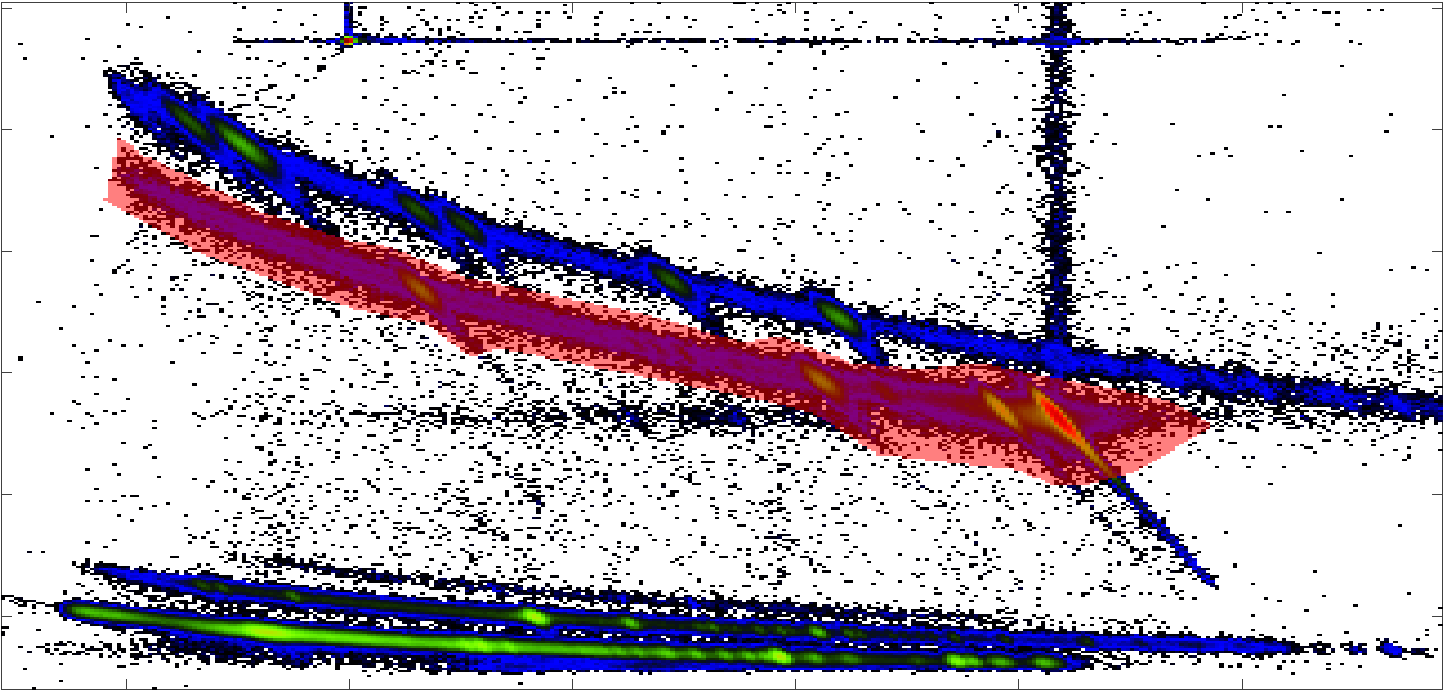
\includegraphics[width=5.5in]{Chapter-6/figs/5deg_SiDEvsSiE.png}};
\node at (-8.0,-2.15) {\rlap{
\includegraphics[scale=0.7]{Chapter-6/figs/9deg_Scale.png}}};

\node[rotate=90] at (-8.0,0) {Si $\Delta$E};
\node at (0,-3.95) {Si E};

\node at (-7.4,-2.6) {\rlap{\footnotesize{50}}};
\node at (-7.55,-2.6+\yTS) {\rlap{\footnotesize{100}}};
\node at (-7.55,{-2.6+(2*\yTS)}) {\rlap{\footnotesize{150}}};
\node at (-7.55,{-2.6+(3*\yTS)}) {\rlap{\footnotesize{200}}};
\node at (-7.55,{-2.6+(4*\yTS)}) {\rlap{\footnotesize{250}}};
\node at (-7.55,{-2.6+(5*\yTS)}) {\rlap{\footnotesize{300}}};

\node at (-6.05,-3.55) {\rlap{\footnotesize{100}}};
\node at (-6.05+\xTS,-3.55) {\rlap{\footnotesize{150}}};
\node at ({-6.05+(2*\xTS)},-3.55) {\rlap{\footnotesize{200}}};
\node at ({-6.05+(3*\xTS)},-3.55) {\rlap{\footnotesize{250}}};
\node at ({-6.05+(4*\xTS)},-3.55) {\rlap{\footnotesize{300}}};
\node at ({-6.05+(5*\xTS)},-3.55) {\rlap{\footnotesize{350}}};

\node at (-8.65-\sl,-1.35+\su) {\rlap{\scriptsize{279964}}};
\node at (-8.50-\sl,-1.62+\su) {\rlap{\scriptsize{46654}}};
\node at (-8.35-\sl,-1.92+\su) {\rlap{\scriptsize{7776}}};
\node at (-8.35-\sl,-2.22+\su) {\rlap{\scriptsize{1296}}};
\node at (-8.20-\sl,-2.52+\su) {\rlap{\scriptsize{216}}};
\node at (-8.05-\sl,-2.82+\su) {\rlap{\scriptsize{36}}};
\node at (-7.90-\sl,-3.12+\su) {\rlap{\scriptsize{6}}};
\node at (-7.90-\sl,-3.42+\su) {\rlap{\scriptsize{1}}};
\node at (-7.90-\sl,-3.72+\su) {\rlap{\scriptsize{0}}};

\node at (-6.85,-2.9) {\rlap{\LARGE{$\textbf{p}$}}};
\node at (-6,-1.7) {\rlap{\LARGE{$\textbf{d}$}}};
\node at (-0.72,-2) {\rlap{\LARGE{$\textbf{t}$}}};
\node at (4.3,-1.4) {\rlap{\LARGE{$^{\textbf{3}}$\textbf{He}}}};
\node at (1.1,1) {\rlap{\LARGE{$^{\textbf{4}}$\textbf{He}}}};

\end{tikzpicture}
\caption{\label{fig:5deg_SiDEvsSiE}A 2D histogram of the Si $\Delta$E vs Si E detector signals. Different groups correspond to different particles depending on their mass and charge. The $^{3}$He group, highlighted in red, is being gated on in the figure.}
\end{figure}

To obtain the $^{39}\mathrm{K}(^{3}\mathrm{He}, {}^{3}\mathrm{He})^{39}\mathrm{K}$ Si detector yield, the gated Si $\Delta$E vs Si E spectrum is first transformed. The regions corresponding to the individual scattering elements all have the same slope, and by rotating them so that they vertically align with the $y$-axis, they can be projected onto the $x$-axis to create a new 1D histogram with narrow peaks. This transformation is equivalent to finding the total energy deposited in the silicon detectors,
\begin{equation} \label{eqn:Si_Slope}
E^{\mathrm{tot}} = \frac{E + p_{\mathrm{Si}}\Delta E}{1 + p_{\mathrm{Si}}},
\end{equation}

\def\yTS{0.686} % y tick space
\def\xTS{1.875} % x tick space
\def\sl{0.38} % shift left
\def\su{0.4} % shift up
\begin{figure}[t]
\centering
\begin{tikzpicture}[scale=0.8, every node/.style={transform shape}]
\node at (0,0) {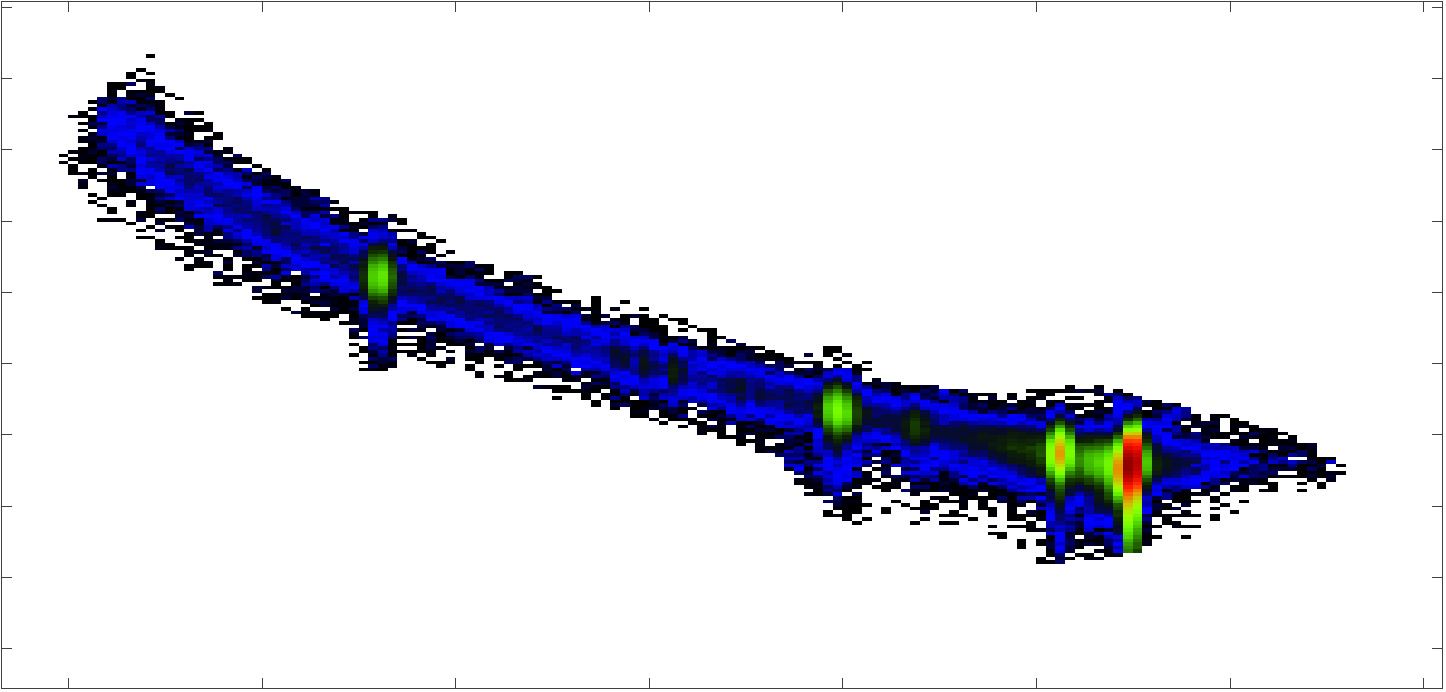
\includegraphics[width=5.5in]{Chapter-6/figs/5deg_SiDEvsSiTotE_GSiDEvsSiE.png}};
\node at (-8.1,-2.35) {\rlap{
\includegraphics[scale=0.75]{Chapter-6/figs/9deg_Scale.png}}};
\node[rotate=90] at (-8.0,0) {Si $\Delta$E};
\node at (0,-3.95) {Si Total E};
\node at (-7.4,-2.9) {\rlap{\footnotesize{80}}};
\node at (-7.55,-2.9+\yTS) {\rlap{\footnotesize{100}}};
\node at (-7.55,{-2.9+(2*\yTS)}) {\rlap{\footnotesize{120}}};
\node at (-7.55,{-2.9+(3*\yTS)}) {\rlap{\footnotesize{140}}};
\node at (-7.55,{-2.9+(4*\yTS)}) {\rlap{\footnotesize{160}}};
\node at (-7.55,{-2.9+(5*\yTS)}) {\rlap{\footnotesize{180}}};
\node at (-7.55,{-2.9+(6*\yTS)}) {\rlap{\footnotesize{200}}};
\node at (-7.55,{-2.9+(7*\yTS)}) {\rlap{\footnotesize{220}}};
\node at (-7.55,{-2.9+(8*\yTS)}) {\rlap{\footnotesize{240}}};
\node at (-7.55,{-2.9+(9*\yTS)}) {\rlap{\footnotesize{260}}};
\node at (-6.63,-3.55) {\rlap{\footnotesize{140}}};
\node at (-6.63+\xTS,-3.55) {\rlap{\footnotesize{160}}};
\node at ({-6.63+(2*\xTS)},-3.55) {\rlap{\footnotesize{180}}};
\node at ({-6.63+(3*\xTS)},-3.55) {\rlap{\footnotesize{200}}};
\node at ({-6.63+(4*\xTS)},-3.55) {\rlap{\footnotesize{220}}};
\node at ({-6.63+(5*\xTS)},-3.55) {\rlap{\footnotesize{240}}};
\node at ({-6.63+(6*\xTS)},-3.55) {\rlap{\footnotesize{260}}};
\node at ({-6.63+(7*\xTS)},-3.55) {\rlap{\footnotesize{280}}};
\node at (-8.65-\sl,-1.35+\su) {\rlap{\scriptsize{390614}}};
\node at (-8.50-\sl,-1.62+\su) {\rlap{\scriptsize{78126}}};
\node at (-8.50-\sl,-1.92+\su) {\rlap{\scriptsize{15625}}};
\node at (-8.35-\sl,-2.22+\su) {\rlap{\scriptsize{3125}}};
\node at (-8.20-\sl,-2.52+\su) {\rlap{\scriptsize{625}}};
\node at (-8.20-\sl,-2.82+\su) {\rlap{\scriptsize{125}}};
\node at (-8.05-\sl,-3.12+\su) {\rlap{\scriptsize{25}}};
\node at (-7.90-\sl,-3.42+\su) {\rlap{\scriptsize{5}}};
\node at (-7.90-\sl,-3.72+\su) {\rlap{\scriptsize{1}}};
\node at (-7.90-\sl,-4.02+\su) {\rlap{\scriptsize{0}}};
\node at (4.0,0.1) {\LARGE{I}};
\node at (3.3,0.2) {\LARGE{K}};
\node at (1.15,0.38) {\LARGE{O}};
\node at (-3.27,1.75) {\LARGE{C}};
\end{tikzpicture}
\caption{\label{fig:5deg_SiDEvsSiTotE}A 2D histogram of the Si $\Delta$E vs Si total E detector signals, gated on the $^{3}$He group and at $\theta_{\mathrm{lab}} = 45^{\circ}$. This is similar to Fig. \ref{fig:5deg_SiDEvsSiE}, except the total Si energy has been calculated based on the slope of the peaks in the Si $\Delta$E vs Si E spectrum (see Eqn. \ref{eqn:Si_Slope}). Each peak is labeled with its corresponding elastic scattering element.}
\end{figure}

\def\yTS{1.85} % y tick space
\def\xTS{1.858} % x tick space
\def\sl{0.38} % shift left
\def\su{0.4} % shift up
\begin{figure}[t]
\centering
\begin{tikzpicture}[scale=0.8, every node/.style={transform shape}]
\node at (0,0) {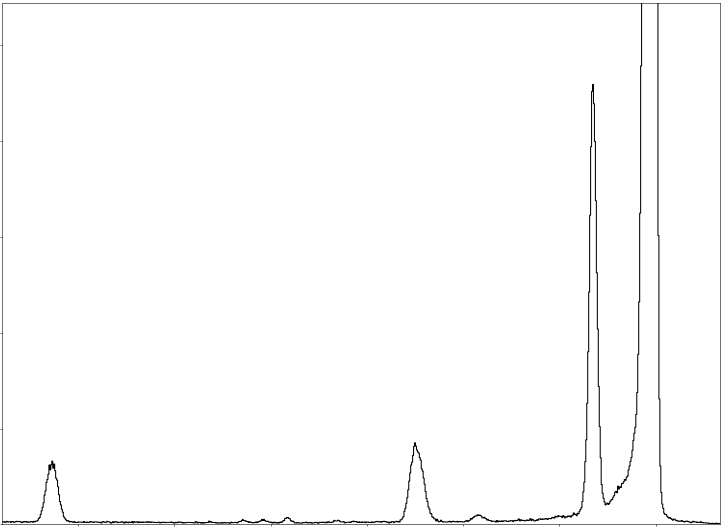
\includegraphics[width=5.5in]{Chapter-6/figs/5deg_SiTotE_GSiDEvsSiE.png}};
\node[rotate=90] at (-8.2,0) {Si Total E Counts};
\node at (0,-5.7) {Channel};
\node at (-7.75,-3.15) {\rlap{\footnotesize{2000}}};
\node at (-7.75,-3.15+\yTS) {\rlap{\footnotesize{4000}}};
\node at (-7.75,{-3.15+(2*\yTS)}) {\rlap{\footnotesize{6000}}};
\node at (-7.75,{-3.15+(3*\yTS)}) {\rlap{\footnotesize{8000}}};
\node at (-7.9,{-3.15+(4*\yTS)}) {\rlap{\footnotesize{10000}}};
\node at (-5.85,-5.28) {\rlap{\footnotesize{1400}}};
\node at (-5.85+\xTS,-5.28) {\rlap{\footnotesize{1500}}};
\node at ({-5.85+(2*\xTS)},-5.28) {\rlap{\footnotesize{1600}}};
\node at ({-5.85+(3*\xTS)},-5.28) {\rlap{\footnotesize{1700}}};
\node at ({-5.85+(4*\xTS)},-5.28) {\rlap{\footnotesize{1800}}};
\node at ({-5.85+(5*\xTS)},-5.28) {\rlap{\footnotesize{1900}}};
\node at ({-5.85+(6*\xTS)},-5.28) {\rlap{\footnotesize{2000}}};
\node at (6,2) {\LARGE{I}};
\node at (4,1) {\LARGE{K}};
\node at (1.65,-4) {\LARGE{O}};
\node at (-5.5,-4) {\LARGE{C}};
\end{tikzpicture}
\caption{\label{fig:5deg_SiTotE}A histogram spectrum of Si Total E gated on the $^{3}$He group at $\theta_{\mathrm{lab}} = 45^{\circ}$, obtained by projecting Fig. \ref{fig:5deg_SiDEvsSiTotE} onto its $x$-axis. Each peak is labeled with its corresponding elastic scattering element. The individual $^{39}$K and $^{41}$K isotopes are unresolvable.}
\end{figure}

\noindent
where $p_{\mathrm{Si}}$ is the Si slope parameter defined by the user in either \texttt{EngeSpec} or \texttt{Jam}. The transformed 2D Si $\Delta$E vs Si total E spectrum, gated on the $^{3}$He group, is shown in Fig. \ref{fig:5deg_SiDEvsSiTotE}. The scattering elements are labaled with their element symbols. Finally, the projected 1D histogram for Si total E is presented in Fig. \ref{fig:5deg_SiTotE}, where the potassium (K) peak can be seen on the shoulder of the iodine (I) peak. The yield of the potassium peak ideally remains constant throughout the experiment, for a given target, since the Si detector telescope is positioned at a constant $\theta_{\mathrm{lab}} = 45^{\circ}$. However, target degradation occurs naturally over time, decreasing the yield of both focal-plane and Si detector measurements. Hence, the normalization corrects for this, as well as the other unknown target properties. 

One complication is the poor resolution between different isotopes for elastic scattering, especially at low angles. In the Si detectors, the potassium peak always consisted of $^{41}$K in addition to $^{39}$K, since a natural KI target was used. In the focal-plane P1 detector, which has better energy resolution, the elastic scattering $^{39}$K peak could be resolved only for $\theta_{\mathrm{lab}} \geq 40^{\circ}$. The presence of $^{41}$K was corrected for in the differential cross-section calculations of $^{39}\mathrm{K}(^{3}\mathrm{He}, {}^{3}\mathrm{He})^{39}\mathrm{K}$ by taking into account both the isotopic abundance ratio of potassium and the relative differential cross-sections of global $^{3}$He OMPs for $^{39}$K and $^{41}$K.

%, as detailed in Section \ref{subsec:SiNorm}.

\subsection{Oxidized Spectra} \label{subsec:oxidized_spectra}

% the first batch of targets (KI $\#$1, KI $\#$2, and KI $\#$3) oxidized at some point during the first day of the experiment, for the $\theta_{\mathrm{lab}} = 5^{\circ}$ and $7^{\circ}$ ($^{3}\mathrm{He},d$) measurements. The focal-plane spectra for these runs consisted of peaks with high-energy tails, expected of targets that undergo oxidation \cite{Landau}. These angles were measured again toward the end of the experiment with the non-oxidized KI $\#$6 target, but the oxidized KI $\#$1 data was not discarded nevertheless. Section \ref{subsec:oxidation} details a novel technique for fitting these spectra.

The KI $\#$1 target was the first one to be used in the $^{39}\mathrm{K}(^{3}\mathrm{He}, d)^{40}\mathrm{Ca}$ experiment at $\theta_{\mathrm{lab}} = 5^{\circ}$ and $7^{\circ}$. It was immediately clear that this target was producing peaks that were not gaussian in the focal-plane P1 spectra, as were the other targets in the first evaporation batch, KI $\#$2 and KI $\#$3. They were transported together and all placed in the target chamber simultaneously. At some point, they were presumably exposed to atmosphere suddenly or for an extended period of time, despite the care taken in transporting them to the target chamber in a sealed box at rough vacuum. The oxidized focal-plane P1 spectrum for all KI $\#$1 runs ($\#15-\#20$) at $\theta_{\mathrm{lab}} = 7^{\circ}$, gated on the deuteron group, are shown sorted together in Fig. \ref{fig:7deg_oxidized}. The low-channel (high-energy) side of each peak has a tail that is potentially smeared over other nearby peaks. This makes fitting peaks very challenging for yield measurements, when high resolution is required. However, Bayesian Monte Carlo techniques were implemented to obtain yield measurements with realistic uncertainties from these runs, as presented in Section \ref{subsec:oxidation}.

\def\yTS{0.69}
\def\xTS{1.945}

\begin{figure}[t]
\centering
\begin{tikzpicture}[scale=1.0, every node/.style={transform shape}]
\node[rotate=90] at (-8.6,0) {P1 Counts};
\node at (0,-3.6) {Channel};
\node at (0,0) {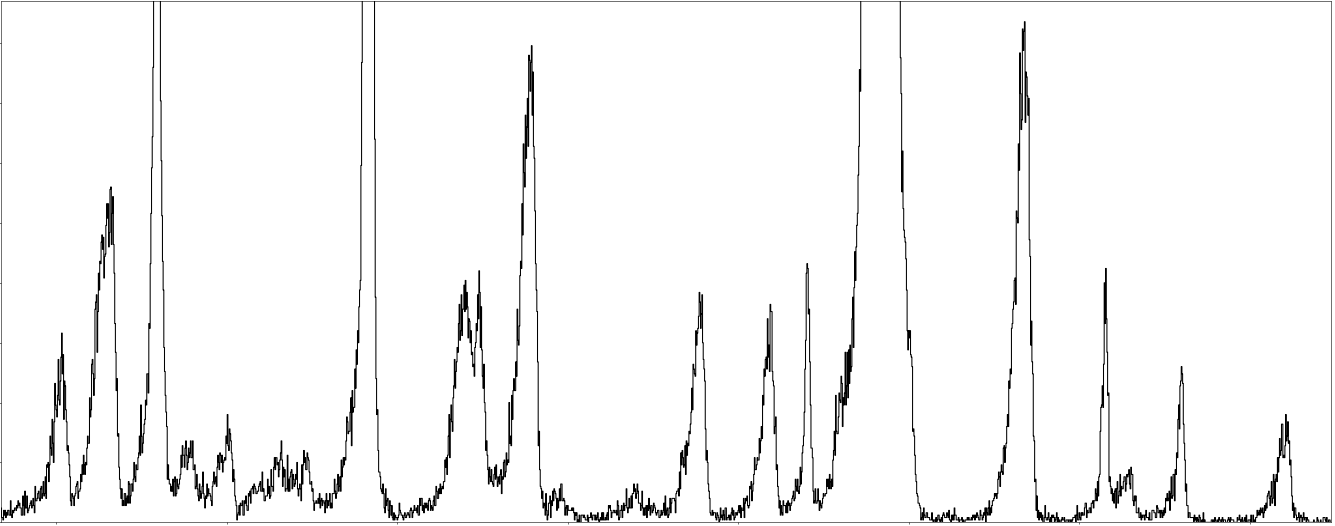
\includegraphics[width=6in]{Chapter-6/figs/7deg_oxidized.png}};
\node at (-7.90,-3.0) {\rlap{\footnotesize{0}}};
\node at (-8.05,-3.0+\yTS) {\rlap{\footnotesize{25}}};
\node at (-8.05,{-3.0+(2*\yTS)}) {\rlap{\footnotesize{50}}};
\node at (-8.05,{-3.0+(3*\yTS)}) {\rlap{\footnotesize{75}}};
\node at (-8.20,{-3.0+(4*\yTS)}) {\rlap{\footnotesize{100}}};
\node at (-8.20,{-3.0+(5*\yTS)}) {\rlap{\footnotesize{125}}};
\node at (-8.20,{-3.0+(6*\yTS)}) {\rlap{\footnotesize{150}}};
\node at (-8.20,{-3.0+(7*\yTS)}) {\rlap{\footnotesize{175}}};
\node at (-8.20,{-3.0+(8*\yTS)}) {\rlap{\footnotesize{200}}};

\node at (-7.32,-3.18) {\rlap{\footnotesize{1250}}};
\node at (-7.32+\xTS,-3.18) {\rlap{\footnotesize{1500}}};
\node at ({-7.32+(2*\xTS)},-3.18) {\rlap{\footnotesize{1750}}};
\node at ({-7.32+(3*\xTS)},-3.18) {\rlap{\footnotesize{2000}}};
\node at ({-7.32+(4*\xTS)},-3.18) {\rlap{\footnotesize{2250}}};
\node at ({-7.32+(5*\xTS)},-3.18) {\rlap{\footnotesize{2500}}};
\node at ({-7.32+(6*\xTS)},-3.18) {\rlap{\footnotesize{2750}}};
\node at ({-7.32+(7*\xTS)},-3.18) {\rlap{\footnotesize{3000}}};

\end{tikzpicture}
\caption{\label{fig:7deg_oxidized}A histogram spectrum of the focal-plane P1  section at $\theta_{\mathrm{lab}} = 7^{\circ}$ with the KI $\#$1 target, gated on the deuteron group. The peaks are clearly not gaussian because of the presence of high-energy (low-channel) tails, a result of oxidation in the KI $\#$1 target.}
\end{figure}

%%%%%%%%%%%%%%%%%%%%%%%%%%%%%%%%%%%%%%%%%%%%%%%%%%%%%%%%%%%%%%%%%%%%%%%%%%%%%%%%%%%%%%%%%%%%%
\section{Bayesian Peak Fitting and Target Oxidation} \label{sec:peak_fitting}

% 1 paragraph overview first here...
The energy loss of light, charged particles through a medium is a statistical process. Particles with the same initial energy will traverse the same length in the medium with a distribution of final energies. This phenomenon is known as energy straggling and was theoretically described by Landau \cite{Landau1944}. Thin-film targets are ideal for high resolution spectral analysis because the energy loss distribution is approximately gaussian. Thick targets, however, alter the energy loss distribution in ways that present challenges to fitting peaks in a spectrum. Section \ref{subsec:peak_fitting_gaus} presents the Bayesian peak fitting procedure implemented in the analysis of the $^{39}\mathrm{K}(^{3}\mathrm{He}, d)^{40}\mathrm{Ca}$ experiment for the case of thin targets, and Section \ref{subsec:oxidation} presents a modified procedure for the case of thick targets, resulting from target oxidation which produces tails in the energy loss distribution.

\subsection{Bayesian Peak Fitting} \label{subsec:peak_fitting_gaus}

Transfer reaction analysis requires precise experimental cross section measurements for each relevant excited state of the residual nucleus. Each cross section is proportional to the yield of the transfer reaction populating the given excited state. An essential ingredient in the yield measurement, described in more detail in Section \ref{sec:cs_calc}, is the number of counts of ejectile particles measured by the focal-plane detector. Each count contributes to a peak along the focal-plane spectrum corresponding to the given excited state with a finite width. The peaks are distinguished by their excitation energies, which are determined through an energy calibration based on their relative centroid positions along the focal-plane, as is done in Section \ref{subsec:cal}. A typical transfer reaction spectrum will include many such peaks, as well as peaks from reactions in the target not necessarily of interest, known as contaminants. As mentioned in the introduction of this section, excited state peaks are typically gaussian-distributed, assuming a thin-film target is used. The spectrum will also include background counts, represented by a straight line. A precise determination of the number of counts in a given peak, in the simplest case, is therefore done by fitting a gaussian with a background line.

The target for the $^{39}\mathrm{K}(^{3}\mathrm{He}, d)^{40}\mathrm{Ca}$ experiment was natural potassium iodine on a natural carbon film backing. The most prominent contaminants were from $(^{3}\mathrm{He}, d)$ reactions on $^{12}$C, $^{13}$C, $^{14}$N, and $^{16}$O, producing excited states from the residual nuclei $^{13}$N, $^{14}$N, $^{15}$O, and $^{17}$F, respectively. The chosen magnetic field of the Enge Split-Pole Spectrograph was such that deuterons from $(^{3}\mathrm{He}, d)$ reactions with iodine were not at all present along the focal-plane, and deuterons from $^{41}\mathrm{K}(^{3}\mathrm{He}, d)$ were only minimally present. However, given the presence of the many other contaminants, and to distinguish doublets, triplets, and other mutliplets, it was deemed necessary to use a more sophisticated technique to fit the peaks from this experiment than a simple chi-squared minimization. Bayesian Monte Carlo sampling was a natural choice, considering its realistic uncertainty handling and flexibility when dealing with non-gaussian fits, presented in Section \ref{subsec:oxidation}. I used the \texttt{BayeSpec} \cite{BayeSpec} graphical user interface (GUI), along with custom Bayesian sampling routines described below, to acquire fits to the $^{39}\mathrm{K}(^{3}\mathrm{He}, d)^{40}\mathrm{Ca}$ data.

% BayeSpec GUI, MCMCGaus
Most peaks from transfer reactions on a thin-film target are gaussian-distributed,
\begin{equation}
    f(x;A,\mu,\sigma) = A \, \exp \Big( -\frac{(x-\mu)^{2}}{2\sigma^{2}} \Big),
\end{equation}
where $A$ is the peak intensity, $\mu$ is its mean, and $\sigma$ is its standard deviation.
%A chi-squared minimization would optimize these 3 parameters to fit the data. Alternatively, 
Bayesian sampling can be used to optimize these 3 parameters to match the focal-plane data if appropriate prior distributions are known. In this case, each prior distribution is approximately normal, $\mathcal{N}(\mu_{0},\sigma_{0}^{2})$, with its own mean $\mu_{0}$ and standard deviation $\sigma_{0}$. Posterior distributions can then be computed from these priors to achieve parameter values with statistically realistic uncertainties that match the data. These more realistic uncertainties make it possible to handle difficult fitting scenarios that would normally cause problems for chi-square minimizations, such as distinguishing peaks in a multiplet with appropriate uncertainties.

Prior means $\mu_{0}$ for $A$ and $\mu$ are particularly simple to obtain if the peak apex is visible. Even if it is not visible, as in the case of a multiplet, a guess can be made for each peak apex location, $(x,y)$, based on the curvature of their sum, where $x$ is the mean guess and $y$ is the intensity guess. Each guess is established by selecting a point using the \texttt{BayeSpec} GUI. The prior standard deviations $\sigma_{0}$ for $A$ and $\mu$ are given constant values conservative enough for sampling to be successful in even the most uncertain cases. These can be adjusted by the user, but are typically left as their defaults, listed below.

The prior mean $\mu_{0}$ and standard deviation $\sigma_{0}$ for $\sigma$ are ideally given constant values for a given reaction representative of most peaks from that reaction in focal-plane spectra. This is because energy loss is nearly equivalent for peaks with similar excitation energies from the same reaction, but it is not equivalent for peaks from different reactions. Therefore, peaks from each reaction should ideally have a shared $\sigma$ prior and a shared $\sigma$ posterior in a single fit if multiple peaks are fit simultaneously. In practice, a single $\sigma$ prior can be used for different reactions if it is conservative enough for sampling to be successful, but the $\sigma$ posteriors should remain different for different reactions. 

A background line must also be included in the model, where its intensity $y_{\mathrm{bg}}$ and slope $m_{\mathrm{bg}}$ have their own $\mathcal{N}(\mu_{0}, \sigma_{0}^{2})$ priors. Put together, the prior distributions for gaussian peaks on a background line in a typical focal-plane spectrum are
\begin{align}
    A_{i} &\sim \mathcal{N}(y_{i}, 10.0^{2}) \nonumber \\
    \mu_{i} &\sim \mathcal{N}(x_{i}, 1.0^{2}) \nonumber \\
    \sigma &\sim \mathcal{N}(5.0, 1.0^{2}) \nonumber \\
    y_{\mathrm{bg}} &\sim \mathcal{N}(\mathrm{max}(1, \mathrm{min}(d)), 0.1^{2}) \nonumber \\
    m_{\mathrm{bg}} &\sim \mathcal{N}(0, 0.01), \label{eqn:gaus_priors}
\end{align}
where $\sigma$ is a constant prior for all reactions, but it can easily be adjusted by the user for different reactions if needed, and $d$ refers to the focal-plane data in the specified fit range. The prior for $m_{\mathrm{bg}}$ can also be adjusted if the background line is clearly not horizontal. The model function to be fit is
\begin{equation}
    f(x;A,\mu,\sigma,y_{\mathrm{bg}},m_{\mathrm{bg}}) = \sum_{i}^{N} A_{i} \, \exp \Big( -\frac{(x-\mu_{i})^{2}}{2\sigma_{\hspace{-0.08cm} j}^{2}} \Big) + \Big(y_{\mathrm{bg}} + m_{\mathrm{bg}} (x - \mathrm{min}(x))\Big), \label{eqn:nGausBkg}
\end{equation}
where $N$ is the total number of gaussian peaks to be fit and $\sigma_{\hspace{-0.08cm} j}$ refers to the shared standard deviation for peaks from reaction $j$.

The posterior computation in the custom Bayesian sampling routine uses the \texttt{quap} function in \texttt{R}, part of the Bayesian \texttt{rethinking} package \cite{Rethinking}. This function finds a quadratic approximation to each full posterior distribution at its mode. It is less sophisticated than Markov Chain Monte Carlo, but its relative simplicity makes it a more efficient option to use with a GUI. The model composed of Eqns. \ref{eqn:gaus_priors} and \ref{eqn:nGausBkg} is provided to \texttt{quap}, which returns the posterior quadratic approximations with built-in uncertainties. Samples from these posteriors are then used to compute the area of each gaussian, given by $\sqrt{2\pi} \, \sigma_{\hspace{-0.08cm} j} A_{i}$, along with their uncertainties. A small number of posterior samples are also used to graphically display the gaussian fits, with different colors representing different reactions.

\begin{figure}[t]
\centering
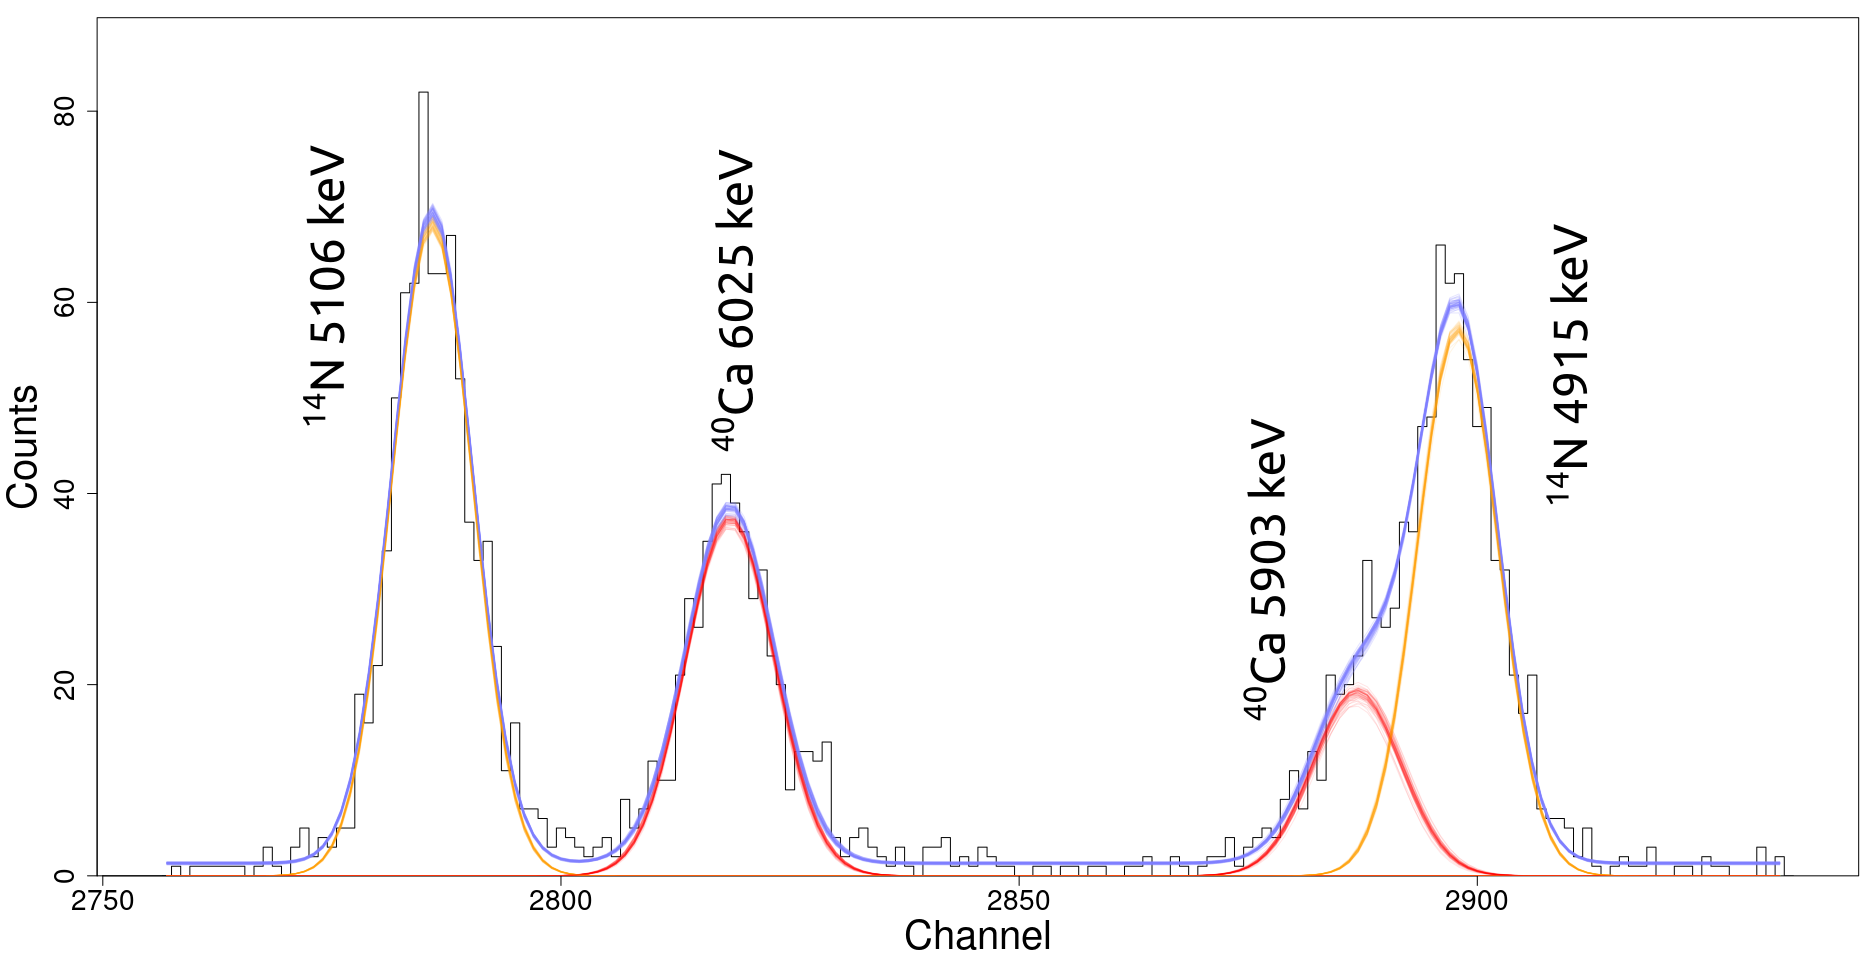
\includegraphics[width=6.5in]{Chapter-6/figs/Gaus_Bayesian.png}
\caption{\label{fig:Gaus_Bayesian}A Bayesian multi-gaussian fit with \texttt{BayeSpec} for the $^{40}$Ca excited states (in red) 6025 keV and 5903 keV from $^{39}\mathrm{K}(^{3}\mathrm{He},d)^{40}\mathrm{Ca}$ and the $^{14}$N excited states (in orange) 5106 keV and 4915 keV from $^{13}\mathrm{C}(^{3}\mathrm{He},d)^{14}\mathrm{N}$ at $\theta_{\mathrm{lab}} = 5^{\circ}$. In red and orange are 50 random samples of the gaussian distributions from the $\sigma$, $\mu$, and $A$ posteriors for each peak. The $^{40}$Ca peaks share an identical $\sigma$ posterior, while the $^{14}$N peaks share their own as well. In blue are the sums of the peaks plus the background line for each of those 50 samples.}
\end{figure}

Figure \ref{fig:Gaus_Bayesian} shows an example of this Bayesian fitting procedure for a $^{39}\mathrm{K}(^{3}\mathrm{He},d)^{40}\mathrm{Ca}$ focal-plane spectrum at $\theta_{\mathrm{lab}} = 5^{\circ}$. Excited states of $^{40}\mathrm{Ca}$ are shown in red and $^{14}\mathrm{N}$ excited state contaminants are shown in orange. In blue is the sum of the gaussians and the background line, given by Eqn. \ref{eqn:nGausBkg}. Each gaussian, as well as the blue curve, consists of 50 individual curves that were sampled from the posteriors to represent the uncertainties. The reason it is useful to combine these 4 peaks into one fit in this example is to better resolve the 5903 keV $^{40}$Ca state in red from the 4915 keV $^{14}$N state in orange in the double gaussian on the right side of the spectrum. The addition of the 6025 keV $^{40}$Ca peak in red and the 5106 keV $^{14}$N peak in orange on the left constrains the $\sigma$ posteriors for the double gaussian. While this may seem like a minor correction, and it is minor in the present example, it is crucial in situations where the double gaussian or multiplet is otherwise impossible to resolve.

%%*****************************************************************************************%%
\subsection{Fitting Peaks with Target Oxidation} \label{subsec:oxidation}

Potassium iodine is hygroscopic, meaning it easily absorbs moisture from the environment. When exposed to atmospheric pressure, the salt slowly oxidizes, forming potassium carbonate and molecular iodine. This oxidation increases the thickness of thin-film targets. The probability of particles traversing the target with large final energies is decreased, introducing a high energy tail in the ejected particle spectrum. The Landau distribution describes this energy loss, but it is computationally challenging to implement. An approximation that has been found to fit oxidized-target spectra well is the exponentially-modified gaussian (EMG) distribution \cite{Babu2016}. The power of the EMG approximation is that its area calculation is the exact same as that of a gaussian distribution, $\sqrt{2\pi} \, \sigma A$, where $\sigma$ and $A$ are parameters of both gaussians and EMGs, but they have slightly different definitions as it will become clear below. This makes it very simple to determine the number of counts for EMG distributions, unlike Landau distributions, where the full area integral must be calculated.

% What to do when the target is oxidized and therefore the peaks have high energy tails. This is called energy straggling and is physically described by the Landau distribution. An approximation to this is an exponentially-modified gaussian 
% Cite: [Measurement of Energy Loss Straggling of Relativistic Electrons in Thin Aluminum Foils, S. Ramesh Babu and N.M. Badiger, ACTA Physica Polonica A. Vol. 129 (2016) DOI: 10.12693/AphysPolA.129.1118  | Page 1119 Section 2.2: Straggling theories of thin absorbers]

The probability density function (PDF) of an EMG distribution $f$ is a convolution of exponential $g$ and gaussian $h$ PDFs,
\begin{align}
    f(x;\sigma,\lambda,\mu,A) = (g*h)(x) &= \int_{-\infty}^{\infty}g(x')h(x-x') \, dx' \\
             &= \int_{0}^{\infty}\lambda \exp\big(-\lambda x'\big) \, A\exp\Big(-\frac{1}{2}\Big(\frac{x-x'-\mu}{\sigma}\Big)^{2}\Big) \, dx' \nonumber \\
             &= A \, \sigma\lambda\sqrt{\frac{\pi}{2}}\exp\Big(\frac{1}{2}(\sigma\lambda)^{2} - (x-\mu)\lambda\Big) \, \mathrm{erfc}\Big(\frac{1}{\sqrt{2}}\Big(\sigma\lambda - \frac{x-\mu}{\sigma}\Big)\Big), \nonumber
\end{align}
where $\lambda$ is the exponential-component rate, $\mu$, $\sigma$, and $A$ are the gaussian-component mean, standard deviation, and peak intensity, respectively, and $\mathrm{erfc}$ is the complimentary error function, defined as $\mathrm{erfc} \, z = 1 - \mathrm{erf} \, z$ for the complex variable $z$, where $\mathrm{erf}$ is the error function,
\begin{equation}
    \mathrm{erf} \, z = \frac{2}{\sqrt{\pi}}\int_{0}^{z}\exp\big(-t^2\big) \, d t.
\end{equation}
The standard EMG distribution, as a function of $x$, has a high--$x$ tail. Since the focal-plane position spectrum channel number is inversely related to energy, the EMG must be modified to have a low--$x$ tail. This is done by simply replacing $x-\mu$ with $\mu-x$ to reflect the standard EMG distribution about its gaussian-component mean, $\mu$. The following discussion of EMG distributions assumes this reflection has been performed.

Previously it was shown for non-oxidized targets that the Bayesian fitting procedure for a gaussian peak requires gaussian mean $\mu$ and peak intensity $A$ priors. The means of these priors are provided by the user when selecting an estimate at the peak apex with the \texttt{BayeSpec} GUI. However, this presents a problem when extending the procedure to EMG fits. An EMG is defined by the $\mu$ and $A$ parameters of its gaussian component, not the mean and peak intensity of the EMG itself. To obtain reasonable priors for the $\mu$ and $A$ parameters, they must be derived from the attributes of the EMG peak apex, where the user selects. This apex defines the mode $x_{m}$ and peak intensity $y_{m}$ of the EMG, which can both be calculated by determining the coordinates where the derivative of the PDF is equal to zero. These are
%The simplest attributes of an EMG from the perspective of the user are the mode $x_{m}$ and peak intensity $y_{m}$, which can also be calculated by determining the coordinates where the derivative of the PDF is equal to zero. These are
\begin{align}
    x_{m} &= \mu - \sigma^{2}\lambda + \sqrt{2} \, \sigma \, z, \nonumber \\
    y_{m} &= A \, \exp \Big( -\frac{1}{2} \Big( \frac{\mu - x_{m}}{\sigma} \Big)^{2} \Big), \label{eqn:mode_peak_intensity}
\end{align}
where $z$ is defined such that
\begin{equation}
    \exp(z^{2}) \, \mathrm{erfc}(z) = \sqrt{\frac{2}{\pi}} \, \frac{1}{\sigma\lambda},
\end{equation}
which can be solved numerically. With $x_{m}$ and $y_{m}$ provided by the user, $\mu$ and $A$ become
\begin{align}
    \mu(\sigma, \lambda) &= x_{m} + \sigma^{2} \lambda - \sqrt{2} \sigma z, \label{eqn:mu_before} \\
    A(\sigma, \lambda) &= y_{m} \exp \Big( \frac{1}{2} \Big( \frac{\mu-x_{m}}{\sigma} \Big)^{2} \Big). \label{eqn:A_before}
\end{align}
The priors would be fully determined if $\sigma$ and $\lambda$, the parameters related to the EMG width and skewness, can be constrained. Fortunately, for a given transfer reaction observed in a focal-plane spectrum, there is little variation between these properties, much like the gaussian $\sigma$ parameter of Section \ref{subsec:peak_fitting_gaus}. From a sample of EMG fits for $^{39}\mathrm{K}(^{3}\mathrm{He},d)^{40}\mathrm{Ca}$ peaks, reasonable priors for $\sigma$ and $\lambda$ were determined to be
\begin{align} 
    \sigma &\sim \mathcal{N}(5.0, \, 1.0^{2}), \label{eqn:sig_prior} \\
    \lambda &\sim \mathcal{N}(0.09, \, 0.02^{2}), \label{eqn:lambda_prior}
\end{align} 
where these are also usually sufficient for other reactions. Priors for Eqns. \ref{eqn:mu_before} and \ref{eqn:A_before} can then be constructed by sampling from Eqns. \ref{eqn:sig_prior} and \ref{eqn:lambda_prior}. The resulting prior distributions for $\mu - x_{m}$ and $A / y_{m}$ are shown in Figure \ref{fig:mu_and_A} in black after taking 10,000 samples from Eqns. \ref{eqn:sig_prior} and \ref{eqn:lambda_prior}. The gaussian approximations (blue) were constructed from the mean and standard deviation of the $\mu - x_{m}$ and $A/y_{m}$ samples, while the lognormal approximations (red) were similarly constructed from the mean and standard deviation of the natural logarithm of those samples. Note that the priors are not gaussian. In fact, the prior for $A / y_{m}$ is neither gaussian nor lognormal. However, a lognormal approximation suffices for both in practice and is preferable to the actual distributions, which are either non-analytical or at least exceedingly complicated. The Bayesian quadratic approximation function, \texttt{quap}, used with \texttt{BayeSpec} requires named prior distributions, forbidding the use of non-analytical distributions. The lognormal approximations also correctly prevent negative sample values and are therefore taken as the priors for $\mu$ and $A$.

\begin{figure}[t]
\centering
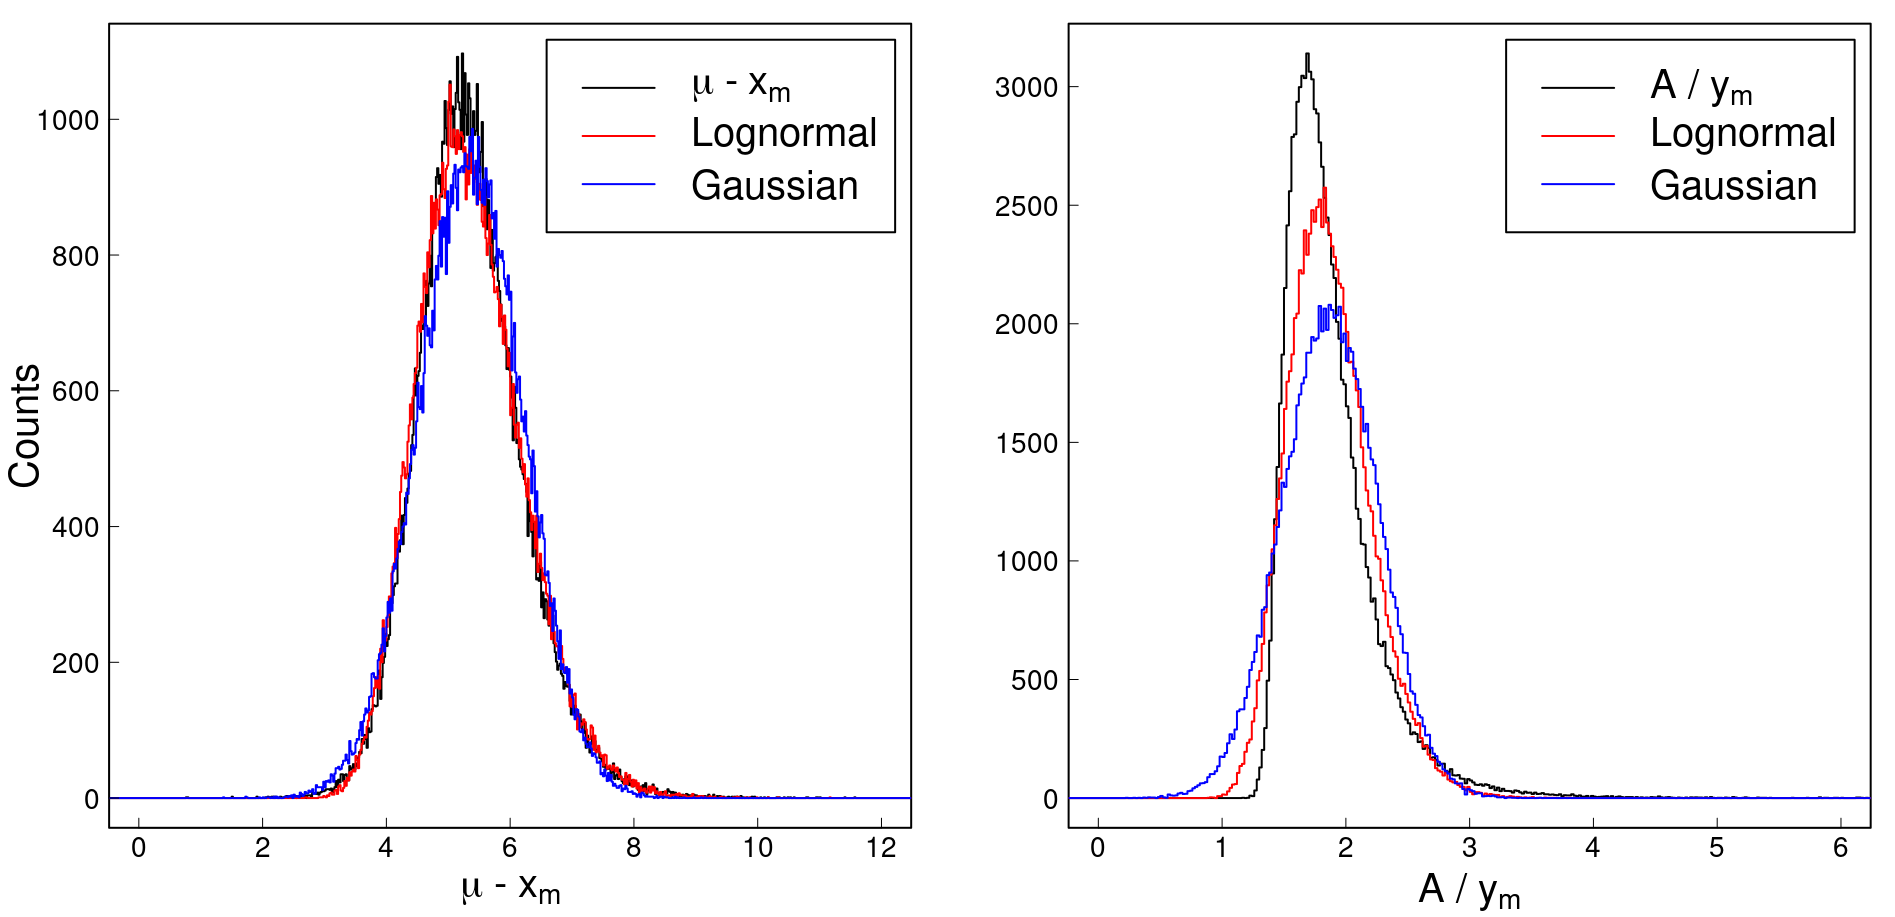
\includegraphics[width=6.5in]{Chapter-6/figs/mu_and_A.png}
\caption{\label{fig:mu_and_A}The constructed priors for $\mu - x_{m}$ (left) and $A/y_{m}$ (right) from 10,000 samples of the $\sigma$ and $\lambda$ priors of Eqns. \ref{eqn:sig_prior} and \ref{eqn:lambda_prior}. The gaussian (blue) approximations were derived from the mean and standard deviation of the samples. The lognormal (red) approximations were derived from the mean and standard deviation of the natural logarithm of those samples.}
\end{figure}

\begin{figure}[t]
\centering
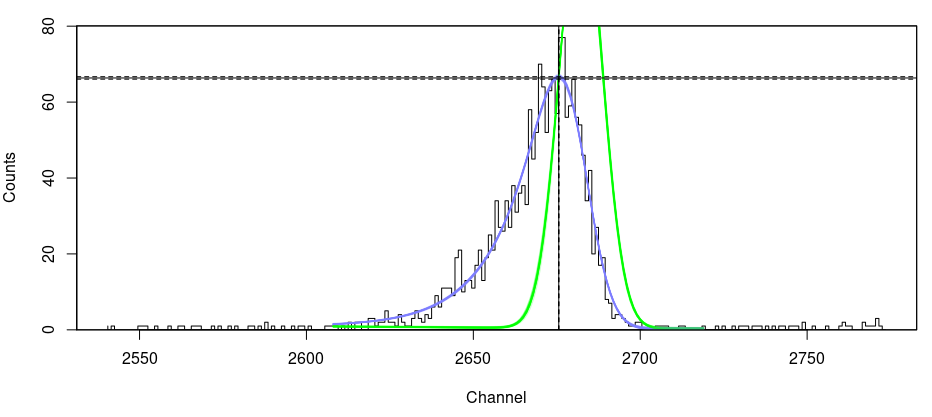
\includegraphics[width=6.5in]{Chapter-6/figs/ExpModGauss_Mode_and_Intensity.png}
\caption{\label{fig:EMG_Mode}A Bayesian exponentially-modified gaussian fit with \texttt{BayeSpec} for the 6285 keV $^{40}\mathrm{Ca}$ state from $^{39}\mathrm{K}(^{3}\mathrm{He},d)^{40}\mathrm{Ca}$ at $\theta_{\mathrm{lab}} = 5^{\circ}$ with an oxidized potassium iodine target (KI $\#$1). In blue are 50 random samples of the exponentially-modified gaussian distribution from the $\sigma$, $\lambda$, $\mu$, and $A$ posteriors, plus the background line. In green are the gaussian components of the exponentially-modified gaussian samples. The new mode and peak intensity are represented by the black lines, where the solid line represents their mean and the dashed lines represent their standard deviation.}
%The mode and peak intensity means of the 10,000 samples are shown by solid black lines, while their standard deviations are represented by dashed lines.
\end{figure}

As in Section \ref{subsec:peak_fitting_gaus}, once the priors have been determined, the quadratic approximations to the posteriors are computed with \texttt{quap}, and the fit is constructed from samples of the EMG distribution with those posteriors. An example of this Bayesian EMG fitting method is shown in Figure \ref{fig:EMG_Mode}, where the 6285 keV $^{40}$Ca state from $^{39}\mathrm{K}(^{3}\mathrm{He},d)^{40}\mathrm{Ca}$ at $\theta_{\mathrm{lab}} = 5^{\circ}$ is fit with an EMG distribution because the potassium iodine target for this run (KI $\#$1) had undergone oxidation. %The $\mu$ and $A$ priors of Eqns. \ref{eqn:mu_before} and \ref{eqn:A_before} were obtained by taking 10,000 samples from the $\sigma$ and $\lambda$ priors of Eqns. \ref{eqn:sig_prior} and \ref{eqn:lambda_prior} and approximating this as a lognormal distribution. 
The closely-packed blue lines are 50 representative samples of the EMG posteriors, plus that of the background line, while the green lines are the corresponding gaussian components of those EMG samples with mean $\mu$, standard deviation $\sigma$, and peak intensity $A$. The new mode and peak intensity from Eqn \ref{eqn:mode_peak_intensity}, obtained by sampling from the posteriors, are shown by the black lines, where the solid line represents its mean and the dashed lines represent its standard deviation. Note that the ($x_{m}$, $y_{m}$) coordinate lies along its gaussian component, a ubiquitous property of EMG distributions. The number of counts in the EMG distribution is simply equivalent to the area of its gaussian component, $\sqrt{2\pi} \, \sigma A$, constructed by sampling from the $\sigma$ and $A$ posteriors.

Figure \ref{fig:EMG_Multiplet} shows how powerful this method can be for high resolution spectral analysis with an oxidized target. The same focal-plane spectrum as Figure \ref{fig:EMG_Mode} is shown here, but it is focused on a region with multiple peaks. The blue summed fit consists of 5 EMG distributions, shown individually by the red and orange lines, and a small, virtually horizontal background line. As before, each distribution shows 50 lines drawn from samples of the EMG posteriors. From a simple energy calibration, the red peaks were found to be $^{40}$Ca excited states with excitation energies 7694 keV, 7658 keV, 7623 keV, and 7532 keV, from left to right, and the orange peak corresponds to the $^{14}$N 6446 keV excited state. Because we expect energy loss to be nearly equivalent for peaks with similar energies from the same reaction, the $\sigma$ and $\lambda$ width and skewness parameter posteriors are fixed between the $^{40}$Ca peaks, while the $^{14}$N peak has its own $\sigma$ and $\lambda$ posteriors. The custom Bayesian sampling routines for both gaussian and EMG fits can be used for a simultaneous fit of any number of peaks from up to 3 different reactions at present, and this could easily be extended to any number of reactions when the need arises.

\begin{figure}
\centering
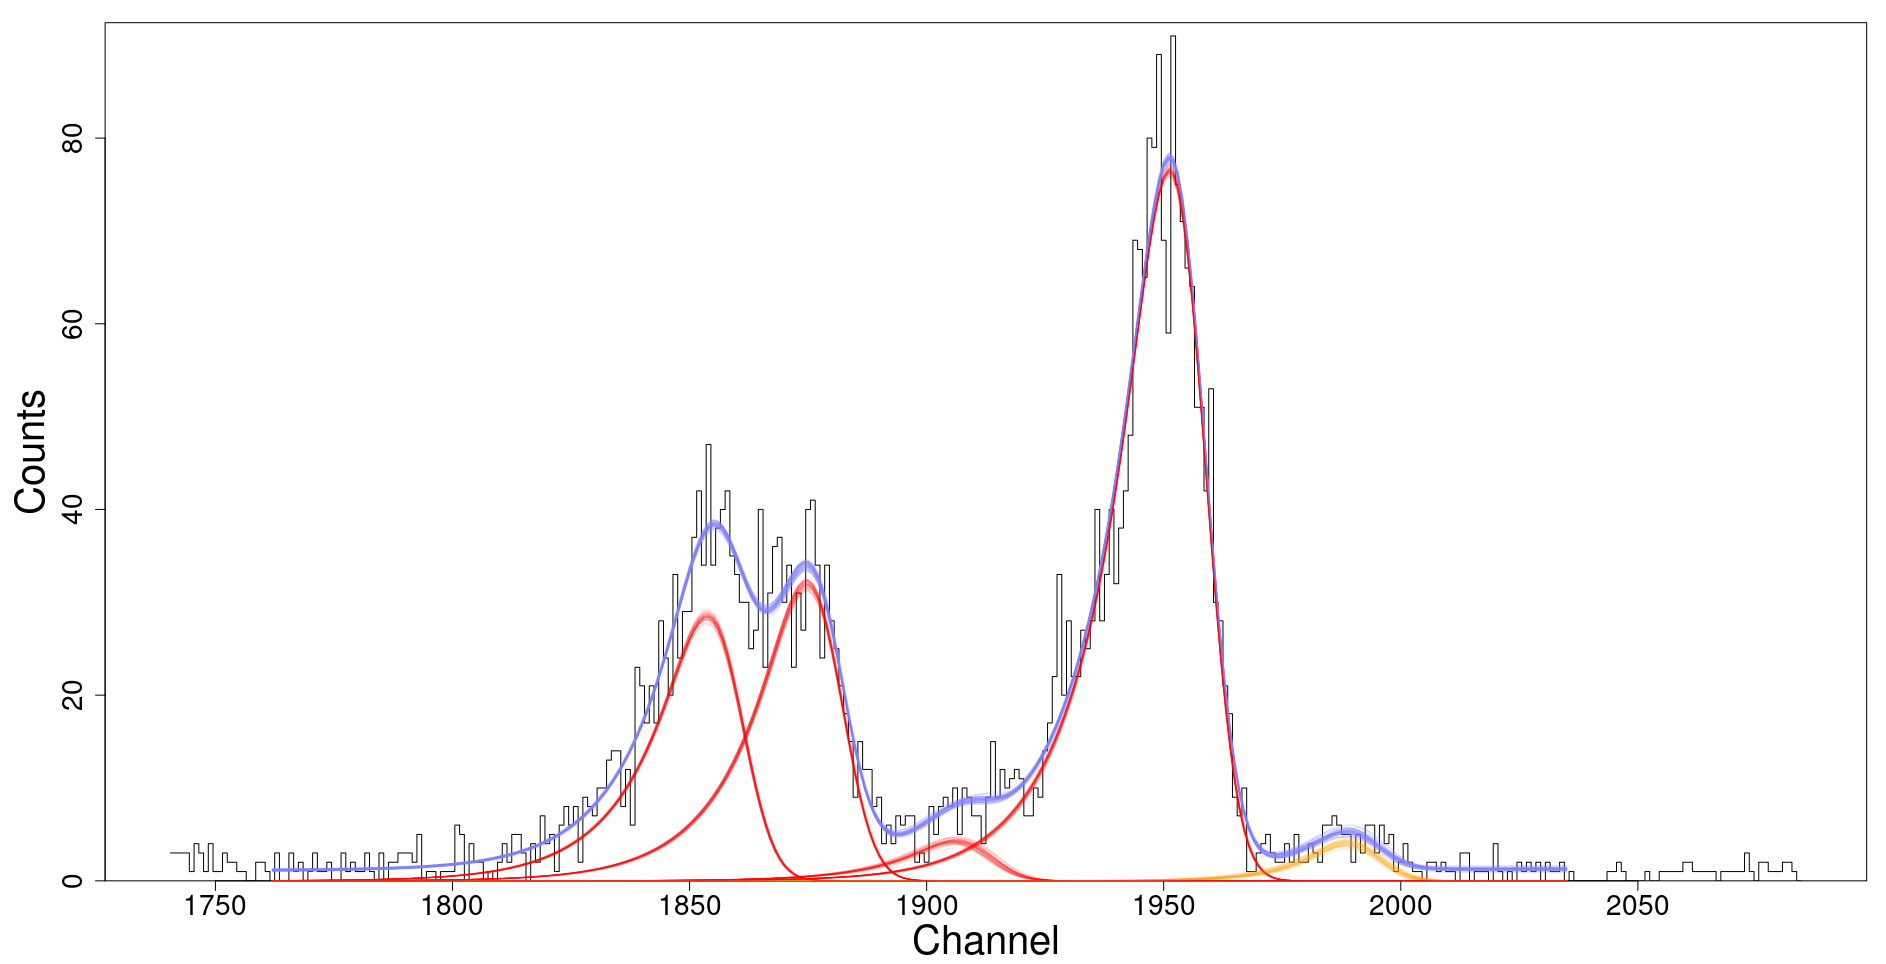
\includegraphics[width=6.5in]{Chapter-6/figs/EMG_Multiplet.png}
\caption{\label{fig:EMG_Multiplet}A Bayesian exponentially-modified gaussian fit with \texttt{BayeSpec} for the $^{40}$Ca excited states (left to right, in red) 7694 keV, 7658 keV, 7623 keV, and 7532 keV from $^{39}\mathrm{K}(^{3}\mathrm{He},d)^{40}\mathrm{Ca}$ and the $^{14}$N excited state (in orange) 6446 keV from $^{13}\mathrm{C}(^{3}\mathrm{He},d)^{14}\mathrm{N}$ at $\theta_{\mathrm{lab}} = 5^{\circ}$ with an oxidized potassium iodine target (KI $\#$1). In red and orange are 50 random samples of the exponentially-modified gaussian distributions from the $\sigma$, $\lambda$, $\mu$, and $A$ posteriors for each peak. The $^{40}$Ca peaks share identical $\sigma$ and $\lambda$ posteriors, whereas the $^{14}$N peak has its own. In blue are the sums of the peaks plus the background line for each of those 50 samples.}
\end{figure}

%Since $x_{m}$ and $y_{m}$ are constant, they can be added and multiplied, respectively, to the resulting normal distributions from the following properties. Consider a normally distributed random variable $X$ with mean $a$ and variance $b^2$. Then the properties
%\begin{align}
%    X + c &\sim \mathcal{N}(a+c,b^{2}), \label{norm_prop1} \\
%    cX &\sim \mathcal{N}(ca,c^{2}b^{2}), \label{norm_prop2}
%\end{align}
%follow from the PDF of the normal distribution for a constant $c$. 

%Taking 10,000 samples from Eqns. \ref{sig_prior} and \ref{lambda_prior}, and using Eqns. \ref{norm_prop1} and \ref{norm_prop2}, Eqns. \ref{mu_before} and \ref{A_before} become
%\begin{align}
%    \mu &\sim \mathcal{N}(x_{m} + 5.37, \, 0.862^{2}) \\
%    A &\sim \mathcal{N}(1.87 y_{m}, \, 0.362^{2} y^{2}_{m}).
%\end{align}

%\begin{equation}
%    z = \mathrm{erfcxinv}\Bigg(\sqrt{\frac{2}{\pi}} \, \frac{1}{\sigma\lambda}\Bigg).
%\end{equation}
%The function $\mathrm{erfcxinv}$ is the inverse of the scaled complementary error function $\mathrm{erfcx}$, defined as
%\begin{equation}
%    \mathrm{erfcx}(z) = \exp(z^{2}) \, \mathrm{erfc}(z).
%\end{equation}
%In other words, $z$ is obtained by sol

%%*****************************************************************************************%%

%%%%%%%%%%%%%%%%%%%%%%%%%%%%%%%%%%%%%%%%%%%%%%%%%%%%%%%%%%%%%%%%%%%%%%%%%%%%%%%%%%%%%%%%%%%%%
\section{Cross Sections} \label{sec:cs_calc}

% Short introduction here...
An essential ingredient in the calculation of thermonuclear reaction rates is the nuclear reaction cross section $\sigma$, introduced in Section \ref{sec:rates}. The reaction cross section is an imaginary, effective area around the target nucleus where the reaction proceeds with a probability of unity if an incident particle passes through it. It is therefore a measure of the probability for a reaction to occur, varying with the incident particle energy. The cross section is closely related to the yield $Y$ of the reaction
\begin{equation}
Y = \frac{N_{\mathrm{R}}}{N_{\mathrm{b}}},
\end{equation}
where $N_{\mathrm{R}}$ is the total number of reactions and $N_{\mathrm{b}}$ is the total number of incident particles. The total number of reactions $N_{\mathrm{R}}$ that occur is related to the number of counts $N_{\mathrm{c}}$, or the area, of a given peak in a detector. However, this peak count is affected by the deadtime $t_{\mathrm{dead}}$ of the data acquisition system. To correct for the deadtime, and therefore get an accurate measure of the number of reactions, the livetime $t_{\mathrm{live}} = 1 - t_{\mathrm{dead}}$ is used as in
\begin{equation}
N_{\mathrm{R}} = \frac{N_{\mathrm{c}}}{t_{\mathrm{live}}}.
\end{equation}
The total number of incident particles $N_{\mathrm{b}}$ is
\begin{equation}
N_{\mathrm{b}} = \frac{q}{Z_{p} \, e},
\end{equation}
where $q$ is the total charge deposited by the incident particles, $Z_{p}$ is the unit charge of the incident particles, and $e$ is the electronic charge (1.6 $\times$ $10^{-19}$ C). The total charge $q$ is derived from the beam-integrated current (BCI) scalar value collected for each pulse during a given run. The BCI has an associated $\mathrm{BCI}_{\mathrm{scale}}$ setting that determines the scale of the deposited charge, which can be adjusted on the beam current readout module. For the $^{39}\mathrm{K}(^{3}\mathrm{He},d)^{40}\mathrm{Ca}$ experiment, the $\mathrm{BCI}_{\mathrm{scale}}$ setting was $10^{-10}$ C/pulse. The number of incident particles $N_{\mathrm{b}}$ is therefore
\begin{equation}
N_{\mathrm{b}} = \frac{\mathrm{BCI} \times \mathrm{BCI_{\mathrm{scale}}}}{Z_{p} \, e}.
\end{equation}
As described in Section \ref{subsec:cs_calc}, the conversion between the yield and the cross section depends on the target thickness $\Delta$E (in energy units) and the stopping power $\mathcal{E} = -(1/N_{\mathrm{t}})dE/dx$ (in units of eV $\mathrm{cm}^{2} / \mathrm{atom}$), where $N_{\mathrm{t}}$ denotes the number density of target nuclei.

A measurement of the total cross section or total yield would require the full $4\pi$ sr solid angle coverage of detectors around the target to ensure that no emitted particles from the reaction are missed. Since this is usually not feasible, the alternative is the measurement of a differential cross section $d\sigma/d\Omega_{\theta}$ or differential yield $dY/d\Omega_{\theta}$ from a detector covering a solid angle $\Omega$ collecting the particles ejected at an angle $\theta$ from the incident beam. The differential cross section can be measured at several angles to determine the angular distribution of the reaction. In the case of charged-particle reactions, such as $^{39}\mathrm{K}(^{3}\mathrm{He},d)^{40}\mathrm{Ca}$, each excited state of the recoil nucleus $^{40}$Ca has its own angular distribution that depends theoretically on the single-particle quantum numbers associated with the quantum mechanical selection rules for the transition, presented in Section \ref{subsec:DWBA_Spec}.

\subsection{Yield to Cross Section Conversion} \label{subsec:cs_calc}

For thin targets, where the cross section $\sigma$ and stopping power $\mathcal{E}$ are approximately constant over the target thickness $\Delta$E, the yield $Y$ is proportional to $\sigma$, with a proportionality constant $n_{\mathrm{X}} = \Delta \mathrm{E} / \mathcal{E}$ representing the number of active target nuclei per $\mathrm{cm}^{2}$ in the target compound $\mathrm{X}_{a}\mathrm{Y}_{b}$ \cite{Iliadis2015}. The term \emph{active nuclei} in this sense means the nuclei of interest $\mathrm{X}$ in the target, whereas the term \emph{inactive nuclei} refers to the nuclei not of interest $\mathrm{Y}$ in the target. The number of inactive target nuclei per unit area is defined as $n_{\mathrm{Y}}$, and the ratio $n_{\mathrm{Y}}/n_{\mathrm{X}}$ is equivalent to the target molecule stoichiometry, $b/a$. For compound targets, the effective stopping power $\mathcal{E}_{\mathrm{eff}} = \mathcal{E}_{\mathrm{X}} + n_{\mathrm{Y}}\mathcal{E}_{\mathrm{Y}} / n_{\mathrm{X}}$ must be used. The same proportionality constant 
\begin{equation}
n_{\mathrm{X}} = \frac{\Delta E}{\mathcal{E}_{\mathrm{eff}}}
\end{equation}
also applies to the differential yield and differential cross section. Additionally, as some of the energy of the incident particles $E_{0}$ is lost in the target, the cross section is evaluated at an effective, reduced energy $E_{\mathrm{eff}} = E_{0} - \Delta\mathrm{E}/2$. The conversion between the differential yield and differential cross section therefore becomes
\begin{equation} \label{eqn:yield_to_cross}
\left[ \frac{dY(E_{0})}{d\Omega} \right]_{\theta} = n_{\mathrm{X}} \, \left[ \frac{d\sigma(E_{\mathrm{eff}})}{d\Omega} \right]_{\theta}.
\end{equation}

The number of active nuclei per $\mathrm{cm}^{2}$, $n_{\mathrm{X}}$, can also be expressed in a form more tractable for experiments in the lab system as \cite{Rolfs1988,SetoodehniaThesis}\footnote{The ``yield'' $Y$ defined in Eqns. 3.30 and 3.31 of Ref. \cite{SetoodehniaThesis} is $N_{\mathrm{R}}$, not $N_{\mathrm{R}}/N_{\mathrm{b}}$, even though it describes it as such in the text.}
\begin{equation}
n_{\mathrm{X}} = \frac{\nu N_{A} \Delta x}{A_{t, \, \mathrm{mol}}} \,\,\, [\mathrm{in \,\, cm}^{-2}],
\end{equation}
where $\nu$ is the number of $\mathrm{X}$ atoms per molecule in the target material, $N_{A}$ is Avogadro's number (6.023 $\times$ $10^{23}$ $\mathrm{atoms}/\mathrm{mole}$), $\Delta x$ is the thickness of the target (in g/$\mathrm{cm}^{2}$), and $A_{t, \, \mathrm{mol}}$ is the molecular mass of the target material (in grams).

Combining everything, the differential cross section in units of mb/sr, where 1 b $ = 10^{-24}$ $\mathrm{cm}^{-2}$, measured in the lab system is calculated as
\begin{equation}
\left[ \frac{d\sigma}{d\Omega} \right]_{\theta} = \frac{N_{c} \, Z_{p} \, A_{t, \, \mathrm{mol}}}{(3.75 \times 10^{9}) \, \Omega \, t_{\mathrm{live}} \, \mathrm{BCI} \times \mathrm{BCI}_{\mathrm{scale}} \, \nu \, \Delta x} \, \, \, [\mathrm{in} \, \, \mathrm{mb}/\mathrm{sr}],
\end{equation}
where the solid angle $\Omega$ is in units of msr, all other variables are defined as before, and the factor $e/N_{A}$ has been evaluated and converged into the numerical factor in the denominator.

\subsection{Rutherford Scattering} \label{subsec:Ruth}

For elastic scattering cross section measurements, it is typical to report the cross section as a ratio to the theoretical Rutherford scattering cross section at the same angle. Theoretical elastic scattering cross sections from optical model potentials (OMPs) are also typically given in terms of the Rutherford ratio, depending on the nuclear reaction code. In the coupled-reaction channels code Fresco \cite{Fresco} for example, the Rutherford ratio is the default output of the elastic scattering cross section. 

In the center-of-mass system, the Rutherford scattering cross section is \cite{Iliadis2015}
\begin{align}
\left[ \frac{d\sigma}{d\Omega} \right]^{\mathrm{Ruth}}_{\theta} &= \left( \frac{Z_{p}Z_{t}e^{2}}{4E_{\mathrm{c.m.}}} \right)^{2} \frac{1}{\sin^{4}(\theta_{\mathrm{c.m.}}/2)} \nonumber \\
&= 1.296 \left( \frac{Z_{p}Z_{t}}{E_{\mathrm{c.m.}}} \right)^{2} \frac{1}{\sin^{4}(\theta_{\mathrm{c.m.}}/2)} \, \, \, [\mathrm{in} \, \, \mathrm{mb}/\mathrm{sr}],
\end{align}
where $Z_{p}$ is the unit charge of the incident particles, as before, $Z_{t}$ is the unit charge of the active target nuclei, $E_{\mathrm{c.m.}}$ is the total kinetic energy in the center-of-mass system, in units of MeV, and $\theta_{\mathrm{c.m.}}$ is the angle measured in the center-of-mass system. The elastic scattering cross section measured in the lab system must first be converted to the center-of-mass system before taking the ratio to Rutherford scattering. This conversion is described in Section \ref{subsec:lab_to_cm}.

\subsection{Cross Sections in the Center-of-Mass System} \label{subsec:lab_to_cm}

The incident beam energy $E_{\mathrm{lab}}$, scattering angle $\theta_{\mathrm{lab}}$, and the differential cross section itself $d\sigma/d\Omega_{\theta_{\mathrm{lab}}}$ must be converted to the center-of-mass frame to apply the Rutherford ratio and to compare with theoretical differential cross sections, which are usually given in the center-of-mass frame.

The conversion from the incident beam energy in the lab system $E_{\mathrm{lab}}$ to the total kinetic energy in the center-of-mass system $E_{\mathrm{c.m.}}$ is \cite{Iliadis2015}
\begin{equation}
E_{\mathrm{c.m.}} = E_{\mathrm{lab}} \frac{A_{t}}{A_{t} + A_{p}},
\end{equation}
where $A_{t}$ and $A_{p}$ are the nuclear masses of the active target nucleus and the incident particle nucleus, respectively. However, mass evaluations typically report atomic masses, not nuclear masses. In general, the nuclear masses $A_{\mathrm{Nuc}}$ can be calculated from the reported atomic masses $A_{\mathrm{Atom}}$ as \cite{Wang2021}
\begin{equation}
A_{\mathrm{Nuc}} = A_{\mathrm{Atom}} - Z \, m_{e} + B_{e}(Z),
\end{equation}
where $Z$ is the unit charge of the nucleus, $m_{e}$ is the electron mass  (548579.909065(16) $\times 10^{-9}$ $\mathrm{g}/\mathrm{mole}$ \cite{Huang2021}), and $B_{e}$ is the electron binding energy, found from Ref. \cite{Huang2021} to be calculated as
\begin{equation}
B_{e}(Z) = 14.4381 \, Z^{2.39} + 1.55468 \times 10^{-8} \, Z^{5.35} \, \mathrm{eV}.
\end{equation} 

The lab angle $\theta_{\mathrm{lab}}$ can be converted to the center-of-mass angle $\theta_{\mathrm{c.m.}}$ using the kinematics relation \cite{Iliadis2015}
\begin{equation} \label{eqn:angle_cm}
\cos \theta_{\mathrm{lab}} = \frac{\gamma + \cos \theta_{\mathrm{c.m.}}}{\sqrt{1 + \gamma^{2} + 2\gamma\cos \theta_{\mathrm{c.m.}}}},
\end{equation}
where the $\gamma$ parameter is defined as
\begin{equation}
\gamma = \sqrt{\frac{A_{p}A_{e}E_{\mathrm{lab}}}{A_{r}(A_{e} + A_{r})Q + A_{r}(A_{r} + A_{e} - A_{p})E_{\mathrm{lab}}}},
\end{equation}
with $A_{e}$ and $A_{r}$ representing the nuclear masses of the ejected particle and recoil nucleus, respectively, and $Q$ representing the $Q$-value of the reaction. For elastic scattering, $A_{e} = A_{p}$, $A_{r} = A_{t}$, and $Q=0$, so that $\gamma = A_{p}/A_{t}$. Eqn. \ref{eqn:angle_cm} can be solved numerically or it can be rewritten as a quadratic equation for $\theta_{\mathrm{c.m.}}$, using the positive solution for forward scattering.

The differential cross section is defined such that the same number of ejected particles cross the solid angle $d\Omega_{\mathrm{lab}}$ in the direction $\theta_{\mathrm{lab}}$ as those crossing the solid angle $d\Omega_{\mathrm{c.m.}}$ in the direction $\theta_{\mathrm{c.m.}}$. That is,
\begin{equation}
\left( \frac{d\sigma}{d\Omega} \right)^{\mathrm{lab}}_{\theta_{\mathrm{lab}}} \, d\Omega_{\mathrm{lab}} = \left( \frac{d\sigma}{d\Omega} \right)^{\mathrm{c.m.}}_{\theta_{\mathrm{c.m.}}} \, d\Omega_{\mathrm{c.m.}}.
\end{equation}
Assuming the cross section does not depend on the azimuthal angle, the conversion between the lab and center-of-mass systems is therefore
\begin{equation}
\frac{\left( d\sigma/d\Omega \right)^{\mathrm{c.m.}}_{\theta_{\mathrm{c.m.}}}}{\left( d\sigma/d\Omega \right)^{\mathrm{lab}}_{\theta_{\mathrm{lab}}}} = \frac{d\Omega_{\mathrm{lab}}}{d\Omega_{\mathrm{c.m.}}} = \frac{d(\cos \theta_{\mathrm{lab}})}{d(\cos \theta_{\mathrm{c.m.}})} = \frac{1 + \gamma \cos \theta_{\mathrm{c.m.}}}{\left( 1 + \gamma^{2} + 2 \gamma \cos \theta_{\mathrm{c.m.}} \right)^{3/2}}.
\end{equation}

\subsection{Si Detector Normalization} \label{subsec:SiNorm}

As mentioned in Section \ref{subsec:SiDet}, a Si detector telescope was used to  measure the $^{39}\mathrm{K}(^{3}\mathrm{He}, {}^{3}\mathrm{He})^{39}\mathrm{K}$ elastic scattering differential cross section at a constant $\theta_{\mathrm{lab}} = 45^{\circ}$, while the focal-plane detector was simultaneously measuring the differential cross sections of both $^{39}\mathrm{K}(^{3}\mathrm{He}, {}^{3}\mathrm{He})^{39}\mathrm{K}$ and $^{39}\mathrm{K}(^{3}\mathrm{He}, d)^{40}\mathrm{Ca}$ over multiple $\theta_{\mathrm{lab}}$ angles. The Si detector elastic scattering cross section was used as a normalization to correct for systematic uncertainties associated with unknown target effects during the focal-plane measurements. Although this is a relative measurement, an absolute scale can be established by comparing to optical model predictions, described in Section \ref{subsec:global_norm}.

The reason the relative measurement is effective is due to the conversion factor $n_{\mathrm{X}}$ between the yield and cross section in Eqn. \ref{eqn:yield_to_cross}. Since $n_{\mathrm{X}}$ only depends on the target properties, taking a relative cross section is equivalent to taking a relative yield, where the target properties cancel out. Because of the angular dependence, however, each differential yield (or equivalently, each differential cross section) must first be converted into the center-of-mass system before taking the ratio. The final form of the differential cross-section ratio $R$ in the center-of-mass system becomes
\begin{equation}
R \equiv \frac{\left( d\sigma/d\Omega_{\mathrm{FP}} \right)^{\mathrm{FP}}_{\theta_{\mathrm{c.m.}}}}{\left( d\sigma/d\Omega_{\mathrm{Si}} \right)^{\mathrm{Si}}_{\theta_{\mathrm{Si}}}} = \frac{N^{\mathrm{FP}}_{c} \, \Omega_{\mathrm{Si}}}{\Omega_{\mathrm{FP}} \, N^{\mathrm{Si}}_{c}} \, \frac{1 + \gamma \cos \theta_{\mathrm{c.m.}}}{\left( 1 + \gamma^{2} + 2 \gamma \cos \theta_{\mathrm{c.m.}} \right)^{3/2}} \, \frac{\left( 1 + \gamma^{2} + 2 \gamma \cos \theta_{\mathrm{Si}} \right)^{3/2}}{1 + \gamma \cos \theta_{\mathrm{Si}}},
\end{equation}
where $\theta_{\mathrm{c.m.}}$ is the angle for the focal plane measurement, $\theta_{\mathrm{Si}} = 48.14^{\circ}$ is the center-of-mass angle for the Si measurement ($\theta_{\mathrm{lab}} = 45^{\circ}$), $\Omega_{\mathrm{Si}} = 4.23(4)$ msr, and $\Omega_{\mathrm{FP}} = 1.00(4)$ msr for all runs of the transfer reaction and at angles $\theta_{\mathrm{lab}} \leq 35^{\circ}$ for elastic scattering; otherwise, $\Omega_{\mathrm{FP}} = 0.50(4)$ msr for elastic scattering. Note that the only experimental quantities required with a relative measurement are the number of detector counts $N_{c}$ and the solid angle $\Omega$ that each detector covers, in addition to the quantities making up the center-of-mass conversion. The $u_{R}$ uncertainty is found to be
\begin{equation}
u_{R} = R \sqrt{\left( \frac{u_{N_{c}}}{N_{c}} \right)^{2}_{\mathrm{FP}} + \left( \frac{u_{\Omega}}{\Omega} \right)^{2}_{\mathrm{FP}} + \left( \frac{u_{N_{c}}}{N_{c}} \right)^{2}_{\mathrm{Si}} + \left( \frac{u_{\Omega}}{\Omega} \right)^{2}_{\mathrm{Si}}},
\end{equation}
where the uncertainties in the angle measurement and $\gamma$ are sufficiently small to be neglected.

% Sort groups and weighted average over them at each angle. Variation from average ratio as an additional scatter uncertainty. Oxidation as an additional scatter uncertainty (20%).

Due to the presence of energy shifts in the $^{39}\mathrm{K}(^{3}\mathrm{He},d)^{40}\mathrm{Ca}$ experiment (see Section \ref{subsec:energy_shifts}), the runs usually could not all be sorted together at a given scattering angle. Therefore, there were multiple relative cross sections that needed to be calculated at these angles, one per sort group, and a method of averaging these measurements was necessary. A weighted average over each sort group $i$ at a given angle was deemed appropriate, where the weight is given in terms of the individual relative cross section uncertainties $u_{R}$, as in
\begin{equation}
\bar{R} = \frac{\sum^{n}_{i} R_{i}/u^{2}_{R, i}}{\sum^{n}_{i} 1/u^{2}_{R, i}},
\end{equation}
for $n$ total sort groups at the given angle. This ensures that the more precise measurements are weighted more. The uncertainty in this weighted average is then
\begin{equation}
u_{\bar{R}} = \sqrt{\frac{1}{\sum^{n}_{i} 1/u^{2}_{R, i}}}.
\end{equation}

In calculating the individual relative cross section uncertainties $u_{R}$, it was clear that an additional scatter uncertainty $u_{s}$ was required to accurately account for the variations from the average $R$. The goal was to apply the same fractional scatter uncertainty for all measurements of a given angle, based on the typical deviation from the average $R$ over all $^{40}$Ca states. An example of this is depicted in Fig. \ref{fig:variation}, where the variations from the average $R$, normalized to unity, at $\theta_{\mathrm{lab}} = 13^{\circ}$ are shown over all sort groups and for all $^{40}$Ca states, up to $E_{x} = 8935$ keV. Each color represents a different $^{40}$Ca state. It is clear that the variations from the average are typically no more than about $10\%$, which is also true for the other angles. The variation from the average $R$ is written as
\begin{equation}
\mathrm{var} = \frac{R}{R_{\mathrm{avg}}},
\end{equation}
where each fractional deviation is found from
\begin{equation}
f_{\mathrm{dev}} = | \mathrm{var} - 1 |.
\end{equation}
The average of these fractional deviations $f_{\mathrm{dev,\, avg}}$ over all the $^{40}$Ca states and all sort groups for a given angle is used as the fractional uncertainty applied to the additional scatter,
\begin{equation}
u_{s} = f_{\mathrm{dev,\, avg}} \, R.
\end{equation}
In cases where only one sort group was needed for an angle, the fractional uncertainty was instead obtained by taking $f_{\mathrm{dev,\, avg}}$ for each sort group and $^{40}$Ca state over all angles. 

\begin{figure}[t]
\centering
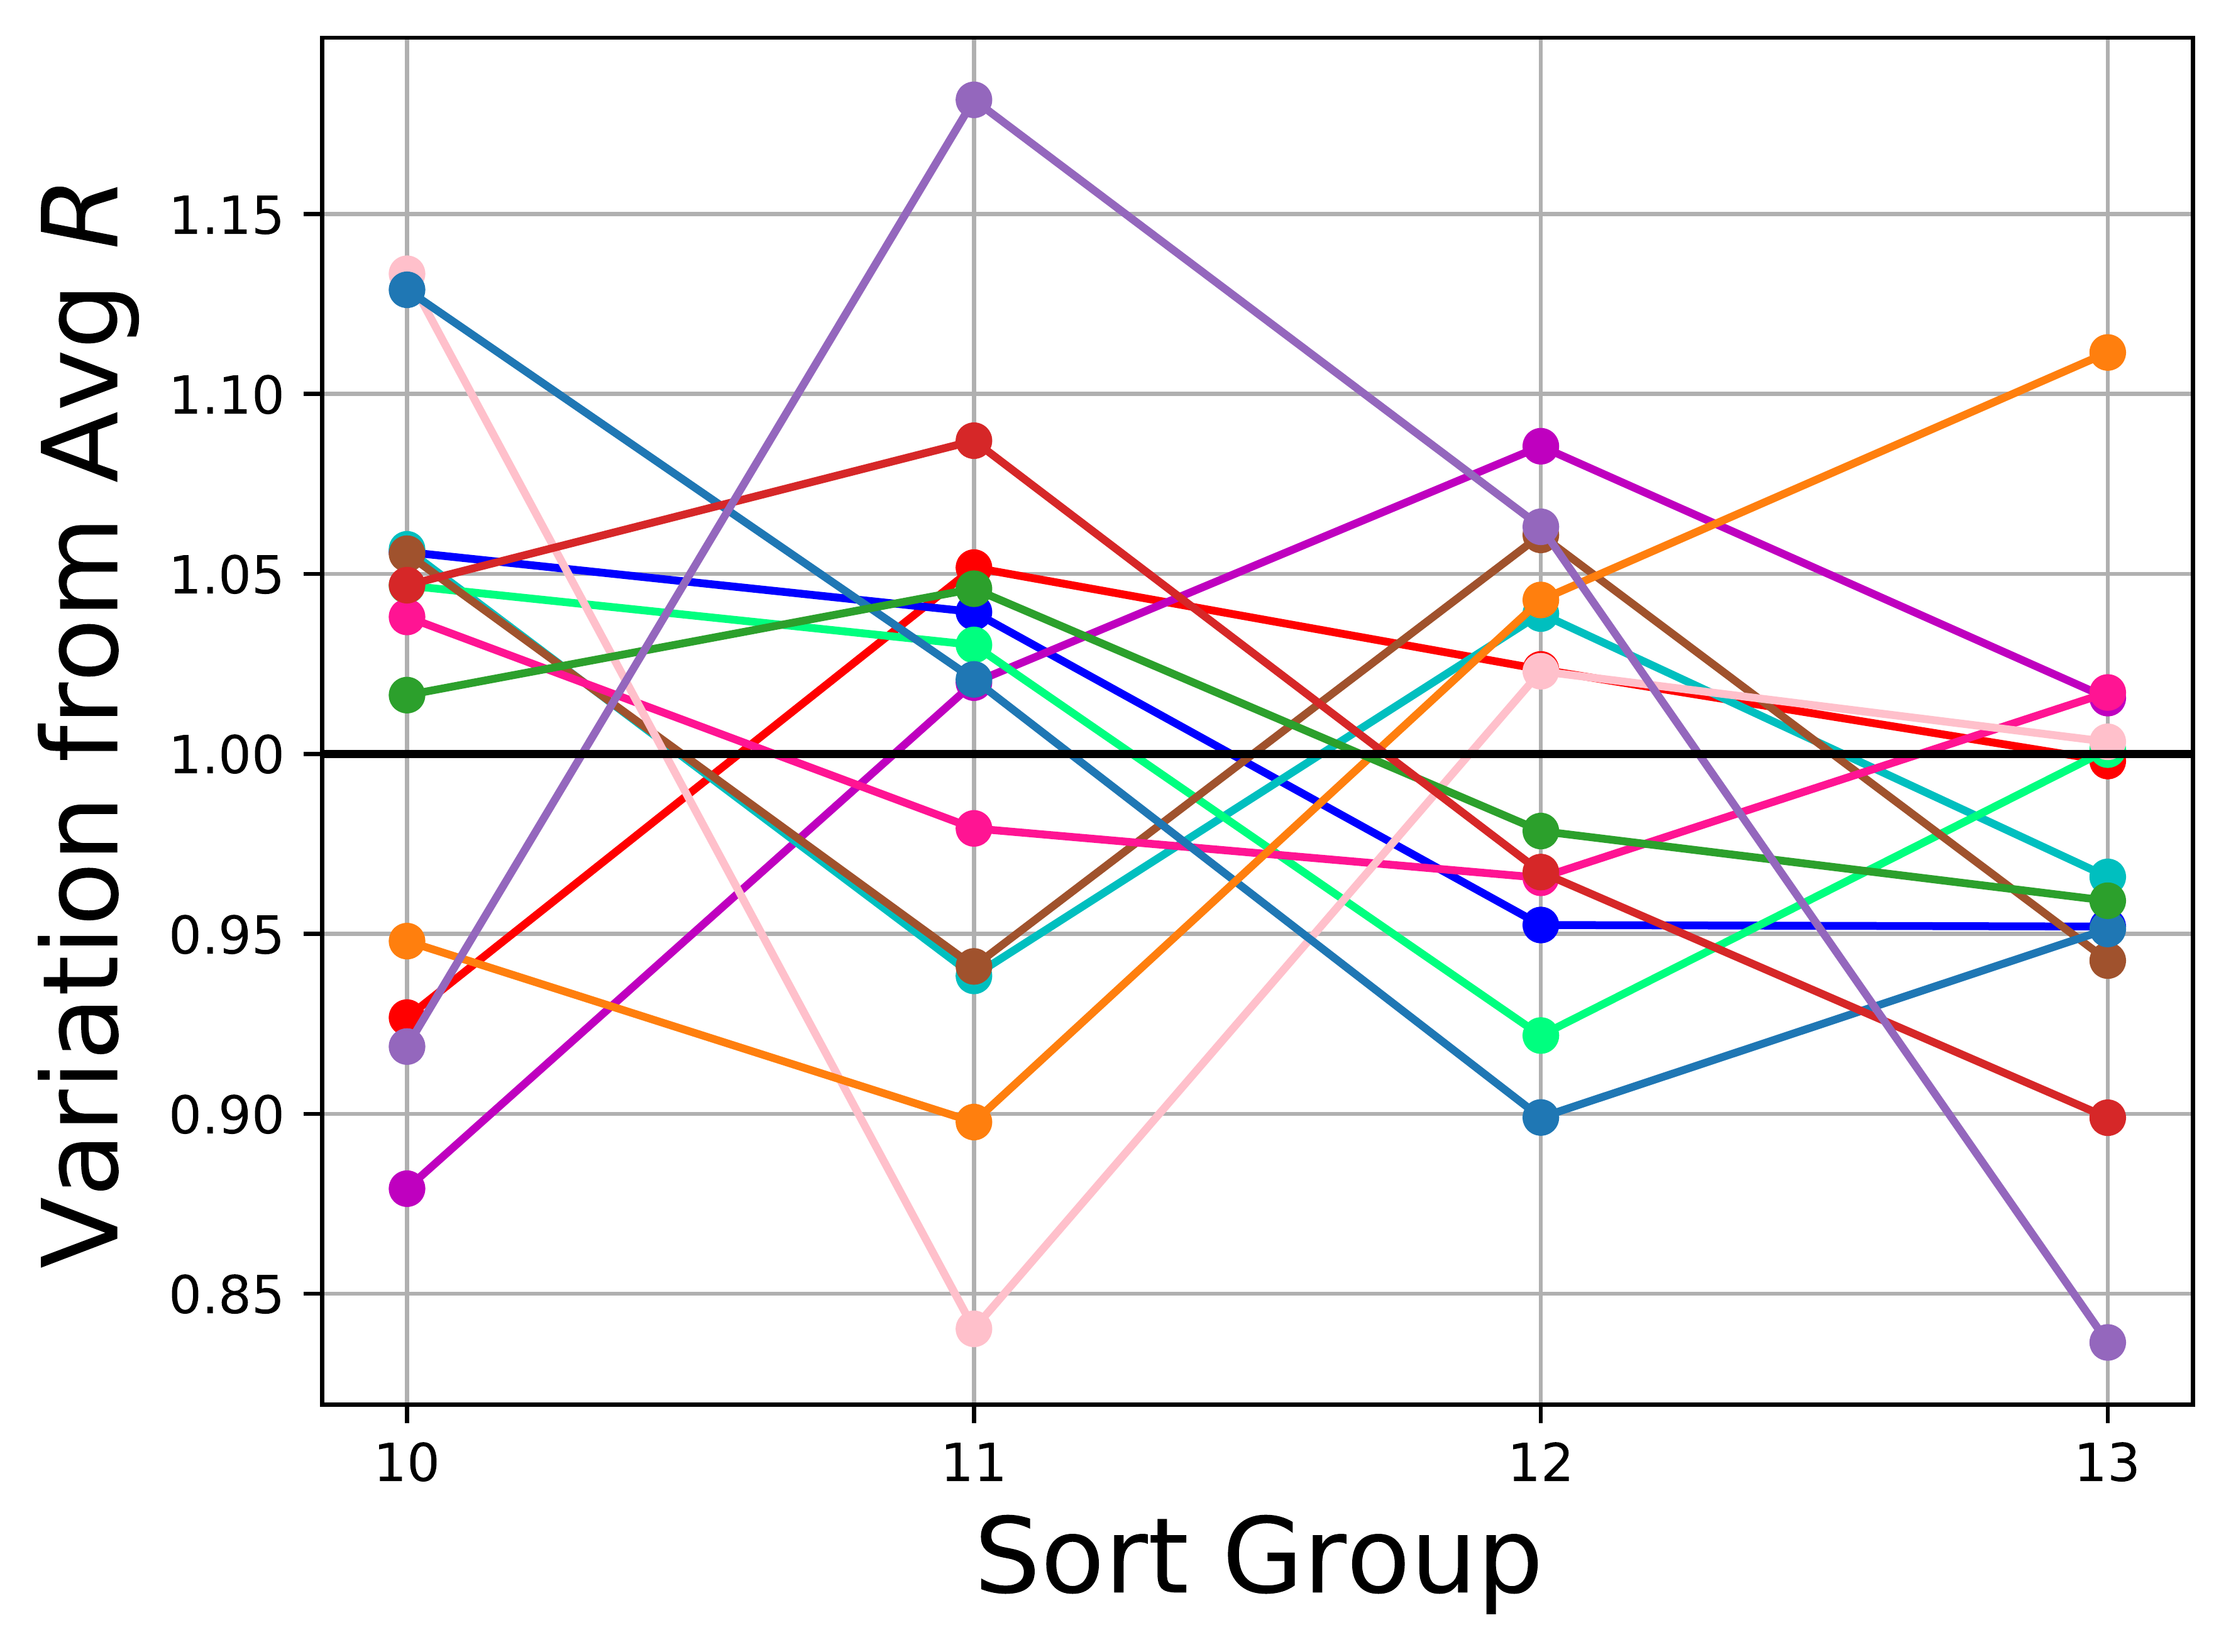
\includegraphics[width=6in]{Chapter-6/figs/variation_13deg.png}
\caption{\label{fig:variation}The variations from the average differential cross-section ratio $R$, normalized to unity, for each sort group over all $^{40}$Ca states measured at $\theta_{\mathrm{lab}} = 13^{\circ}$. The colored lines correspond to each $^{40}$Ca state up to $E_{x} = 8935$ keV. The variations are typically within $10\%$ of the average, which is true for the other angles as well. The average deviation for a given angle is used as an additional scatter uncertainty, as described in the text.}
\end{figure}

For sort groups where an oxidized target (KI $\#$1) was used, it was determined that the uncertainty was still underestimated, based on the tension between measurements at the same angle with targets that were not oxidized. An additional $f_{\mathrm{ox}} = 20\%$ scatter was added in these cases to account for any unknown variability and to apply more weight to measurements with non-oxidized targets. The resulting uncertainty in each $R$ measurement with the added scatter is thus
\begin{equation}
u'^{\, 2}_{R} = u^{2}_{R} + u^{2}_{s} + u^{2}_{\mathrm{ox}} = u^{2}_{R} + (f^{2}_{\mathrm{dev,\, avg}} + f^{2}_{\mathrm{ox}}) \, R^{2},
\end{equation}
where $f_{\mathrm{dev,\, avg}}$ covers all angles in cases where only one sort group was needed for an angle and $f_{\mathrm{ox}} = 0$ for non-oxidized targets. 

\subsection{Optical Model Normalization} \label{subsec:global_norm}

An absolute scale for the relative cross section is established by applying a normalization factor $N_{\mathrm{ES}}$ obtained from the comparison between the measured $^{39}\mathrm{K}(^{3}\mathrm{He}, {}^{3}\mathrm{He})^{40}\mathrm{Ca}$ elastic scattering relative cross section and the absolute cross section from a global $^{3}$He optical model potential for $^{39}$K (see Section \ref{subsec:Optical_Model}, covering optical model potentials). Both of these cross sections are given in terms of a ratio to Rutherford scattering, which is theoretically unity at $\theta_{\mathrm{c.m.}} = 0^{\circ}$.

% Part 1: The Optical Model Potential itself
The global $^{3}$He optical model potential of Ref. \cite{Liang2009} was chosen as the reference for the absolute scale. A global optical model potential is found through an optimization procedure fitting an exhaustive list of experimental elastic scattering data for several target nuclei. In the case of Ref. \cite{Liang2009}, there were 148 sets of elastic scattering data for 52 target nuclei. The potential parameters are expressed as functions of beam energy and target mass. For $^{39}\mathrm{K} + \, {}^{3}\mathrm{He}$ at $E_{\mathrm{lab}} = 21$ MeV, the potential parameters are given in Tabel \ref{tab:OMP_3He}.

\begin{table}[t]
\centering
\caption{\label{tab:OMP_3He}Global optical model potential parameters for $^{39}\mathrm{K} + {}^{3}\mathrm{He}$ at $E_{\mathrm{lab}} = 21$ MeV from Ref. \cite{Liang2009}.}
\begin{tabular}{ccccccc}
\hline\midrule
$V_{r}$ & $r_{r}$ & $a_{r}$ & $W_{v}$ & $r_{v}$ & $a_{v}$ & $W_{s}$\\ \midrule
117.881 & 1.178 & 0.768 & -0.646 & 1.415 & 0.847 & 20.665\\
\hline\hline
\end{tabular}
\begin{tabular}{ccccccc}
$r_{s}$ & $a_{s}$ & $V_{so}$ & $r_{so}$ & $a_{so}$ & $W_{so}$ & $r_{c}$\\ \midrule
1.198 & 0.852 & 2.083 & 0.738 & 0.946 & -1.159 & 1.289\\
\hline\hline
\end{tabular}
\end{table}

%\begin{table}[t]
%\centering
%\caption{\label{tab:OMP_3He}Global optical model potential parameters for $^{39}\mathrm{K} + \,^{3}\mathrm{He}$ at $E_{\mathrm{lab}} = 21$ MeV from Ref. \cite{Liang2009}.}
%\begin{tabular}{llllllllllllll}
%\hline\midrule
%$V_{r}$ & $r_{r}$ & $a_{r}$ & $W_{v}$ & $r_{v}$ & $a_{v}$ & $W_{s}$ & $r_{s}$ & $a_{s}$ & $V_{so}$ & $r_{so}$ & $a_{so}$ & $W_{so}$ & $r_{c}$\\ \midrule
%117.881 & 1.178 & 0.768 & -0.646 & 1.415 & 0.847 & 20.665 & 1.198 & 0.852 & 2.083 & 0.738 & 0.946 & -1.159 & 1.289\\
%\hline\hline
%\end{tabular}
%\end{table}

% Part 2: The non-normalized differential cross sections

% Part 3: The cubic interpolation method for normalization

%The focal plane differential cross-section has been corrected to account for the fact that $^{39}$K and $^{41}$K are unresolvable in the silicon detector peak for potassium and in some angles of the focal plane detector peak for potassium (see text).

\newpage

\begin{figure}
\centering
\begin{tikzpicture}[scale=1.0, every node/.style={transform shape}]
\node at (0,0) {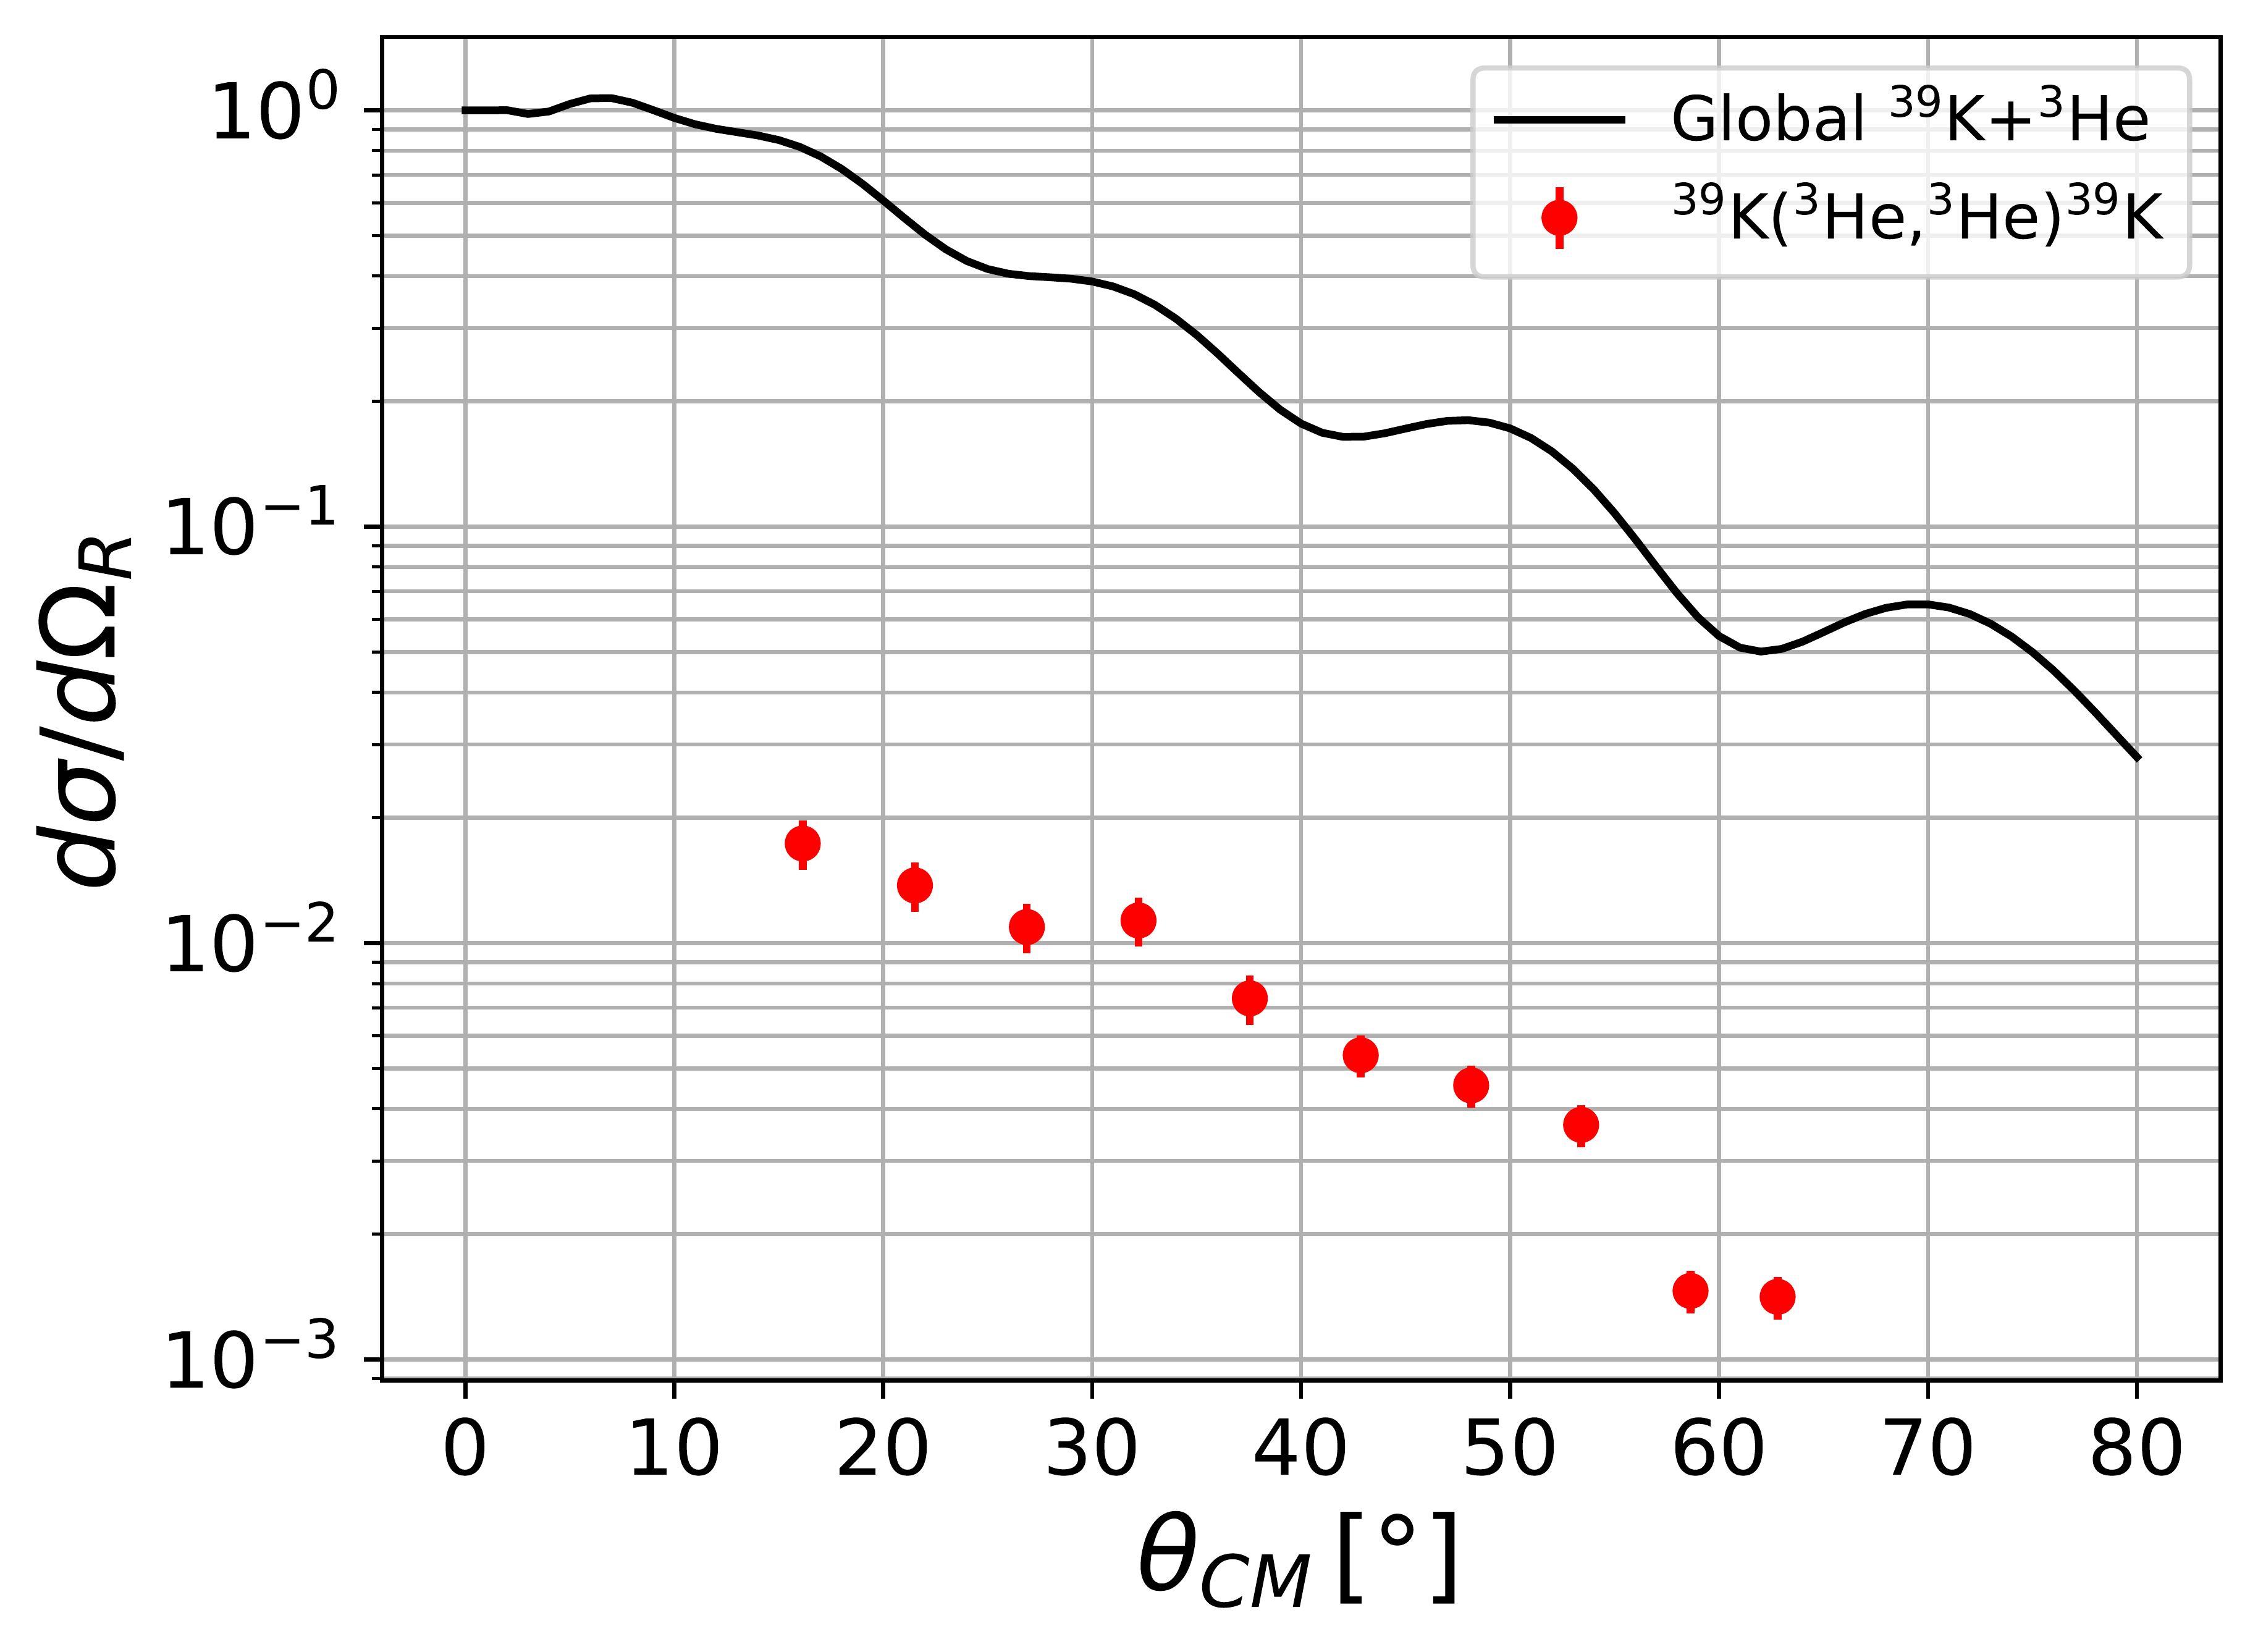
\includegraphics[width=6.5in]{Chapter-6/figs/global_NoNorm.png}};
\node at (0,1.5) {\rlap{\LARGE{$\textbf{N}_{\mathrm{\textbf{ES}}}$}}};
\draw[>=triangle 45, line width = 0.5 mm, <->] (-0.3,3.9) -- (-0.3,-0.9);
\end{tikzpicture}
\caption{\label{fig:ES_NoNorm}The differential cross-section, as a ratio to Rutherford scattering, of the global $^{3}$He optical model potential of Ref. \cite{Liang2009} for $^{39}$K (black line) and that of the present relative $^{39}\mathrm{K}(^{3}\mathrm{He}, {}^{3}\mathrm{He})^{39}\mathrm{K}$ measurements (red data). The scaling factor $N_{\mathrm{ES}}$ is illustrated, which is applied to the transfer data to establish an absolute scale.}
\end{figure}

\newpage

\begin{figure}
\centering
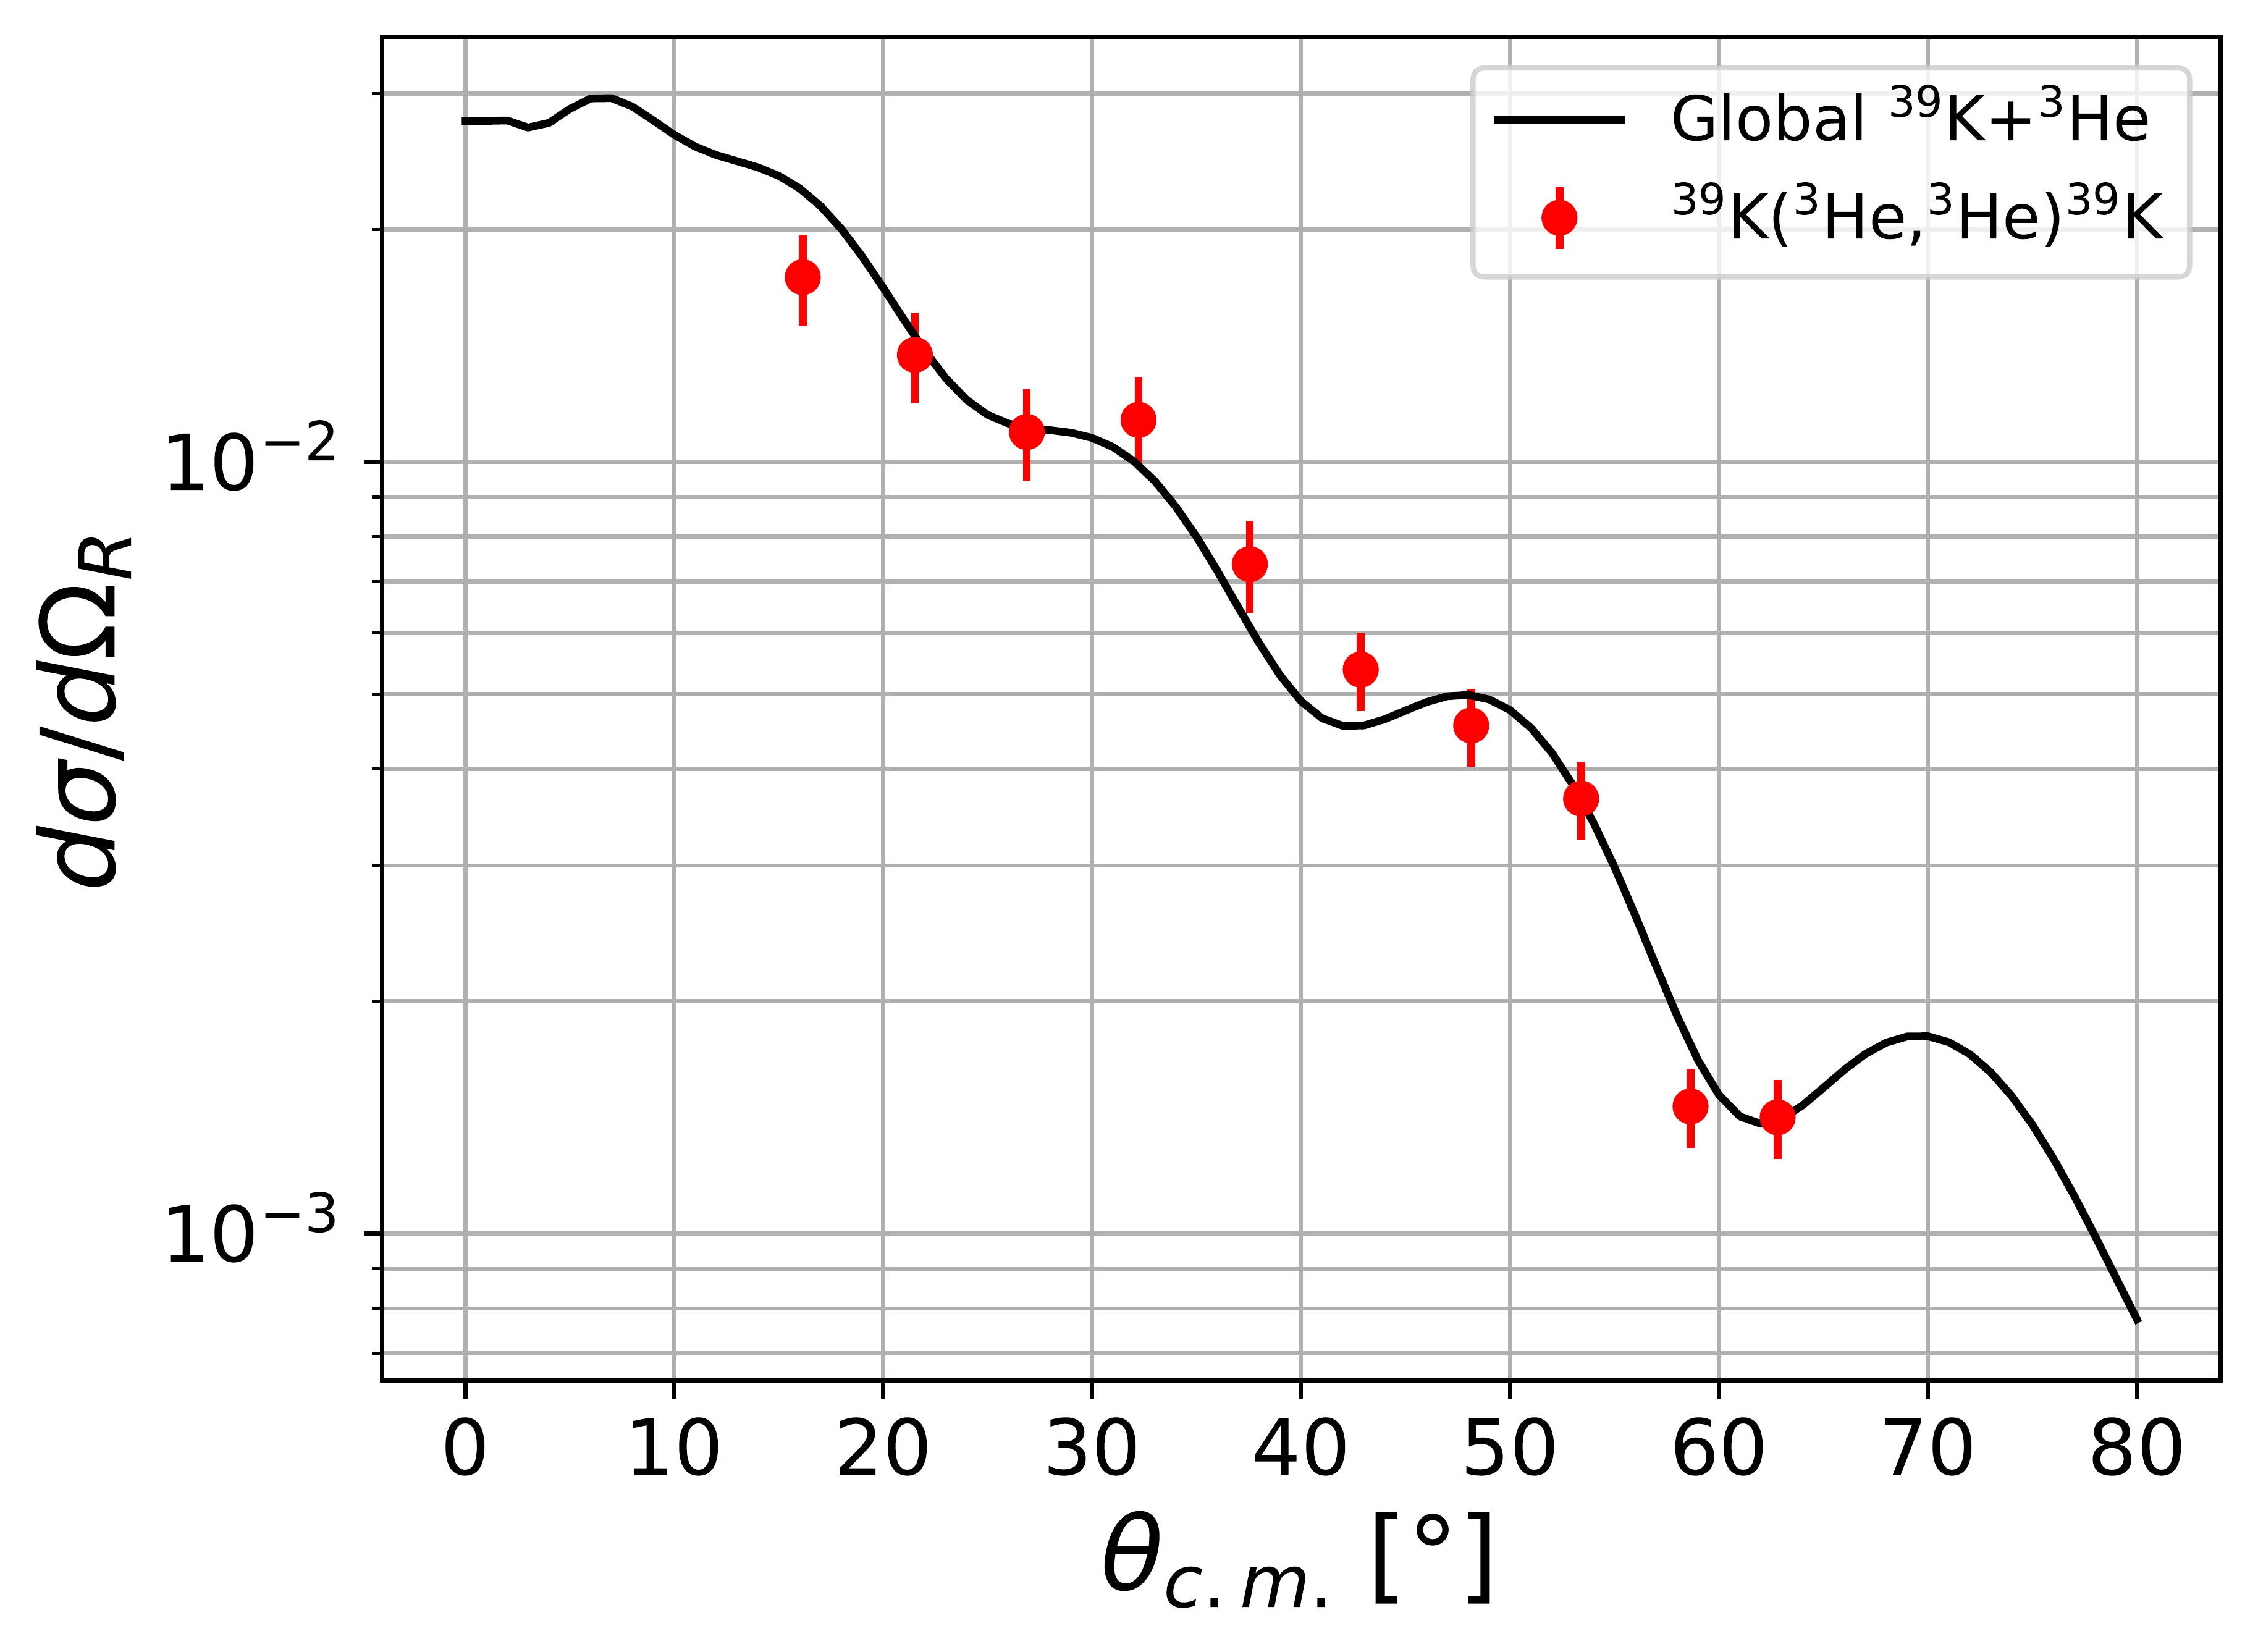
\includegraphics[width=6.5in]{Chapter-6/figs/global_Norm.png}
\caption{\label{fig:ES_Norm}The same as Fig. \ref{fig:ES_NoNorm}, except the differential cross-section of the global $^{3}$He optical model potential has been scaled by $N_{\mathrm{ES}}$ to match the experimental measurements, as described in the text.}
\end{figure}

\newpage

%%%%%%%%%%%%%%%%%%%%%%%%%%%%%%%%%%%%%%%%%%%%%%%%%%%%%%%%%%%%%%%%%%%%%%%%%%%%%%%%%%%%%%%%%%%%%
\section{$^{39}\mathrm{\textbf{K}}(^{3}\mathrm{\textbf{He}},d)^{40}\mathrm{\textbf{Ca}}$ Analysis}

\subsection{Energy Calibrations} \label{subsec:cal}



\subsection{Differential Cross Sections}

\begin{figure*}[t]
\centering
%\begin{tikzpicture}
%%\hspace{0.3cm}
%\node at (-4,0) {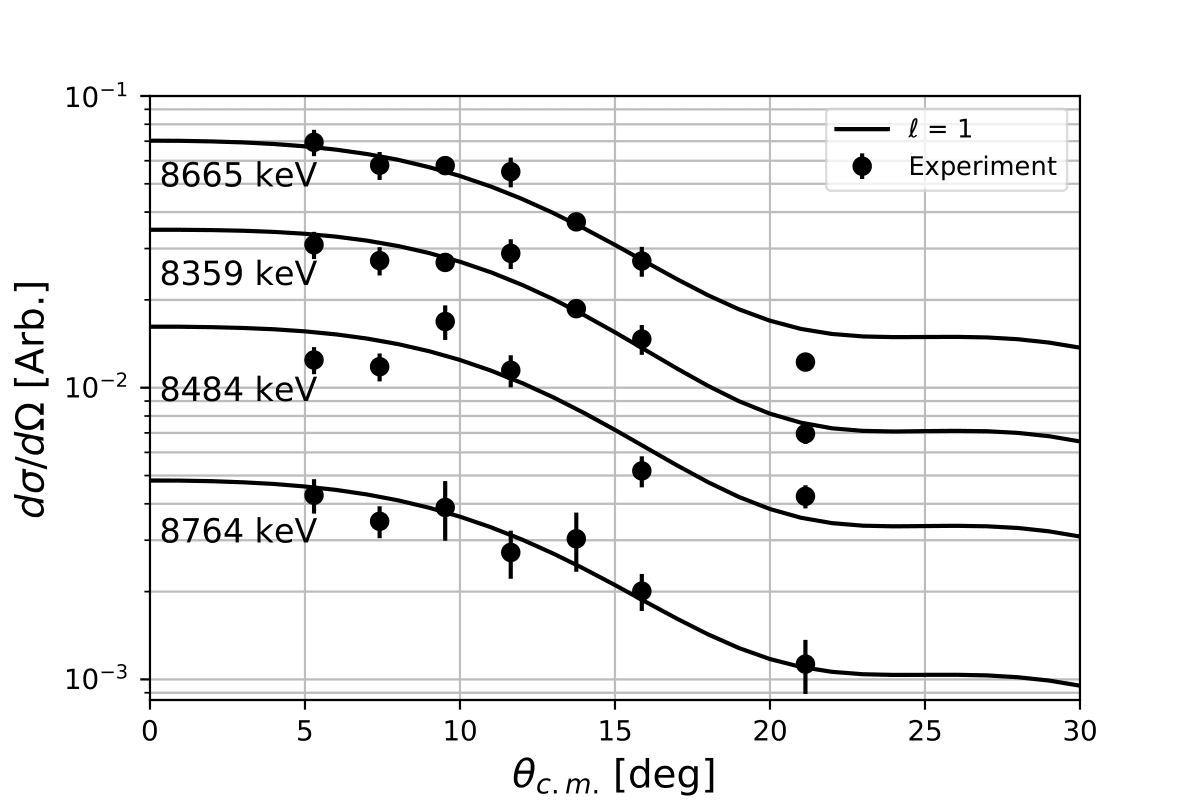
\includegraphics[width=8.6cm]{Chapter-4/figs/unbound_l1.png}};
%\node at (4,0) {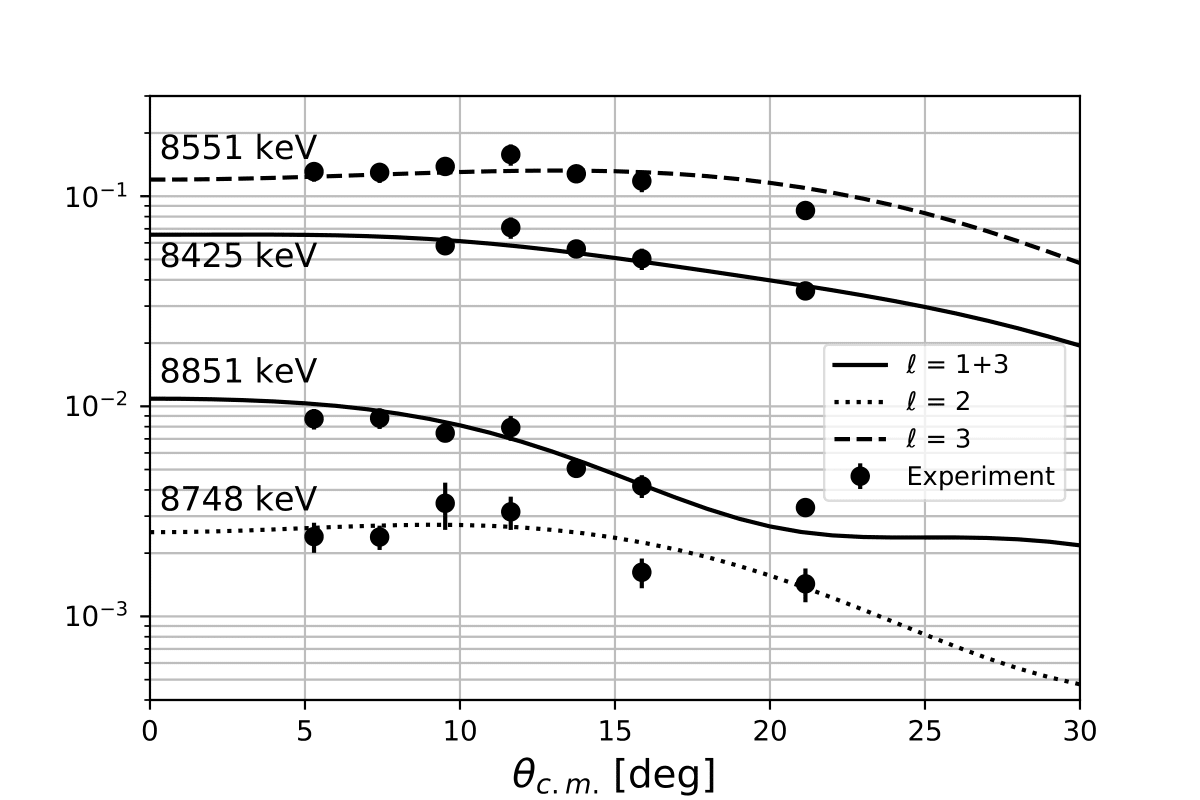
\includegraphics[width=8.6cm]{Chapter-4/figs/unbound_others.png}};
%\end{tikzpicture}
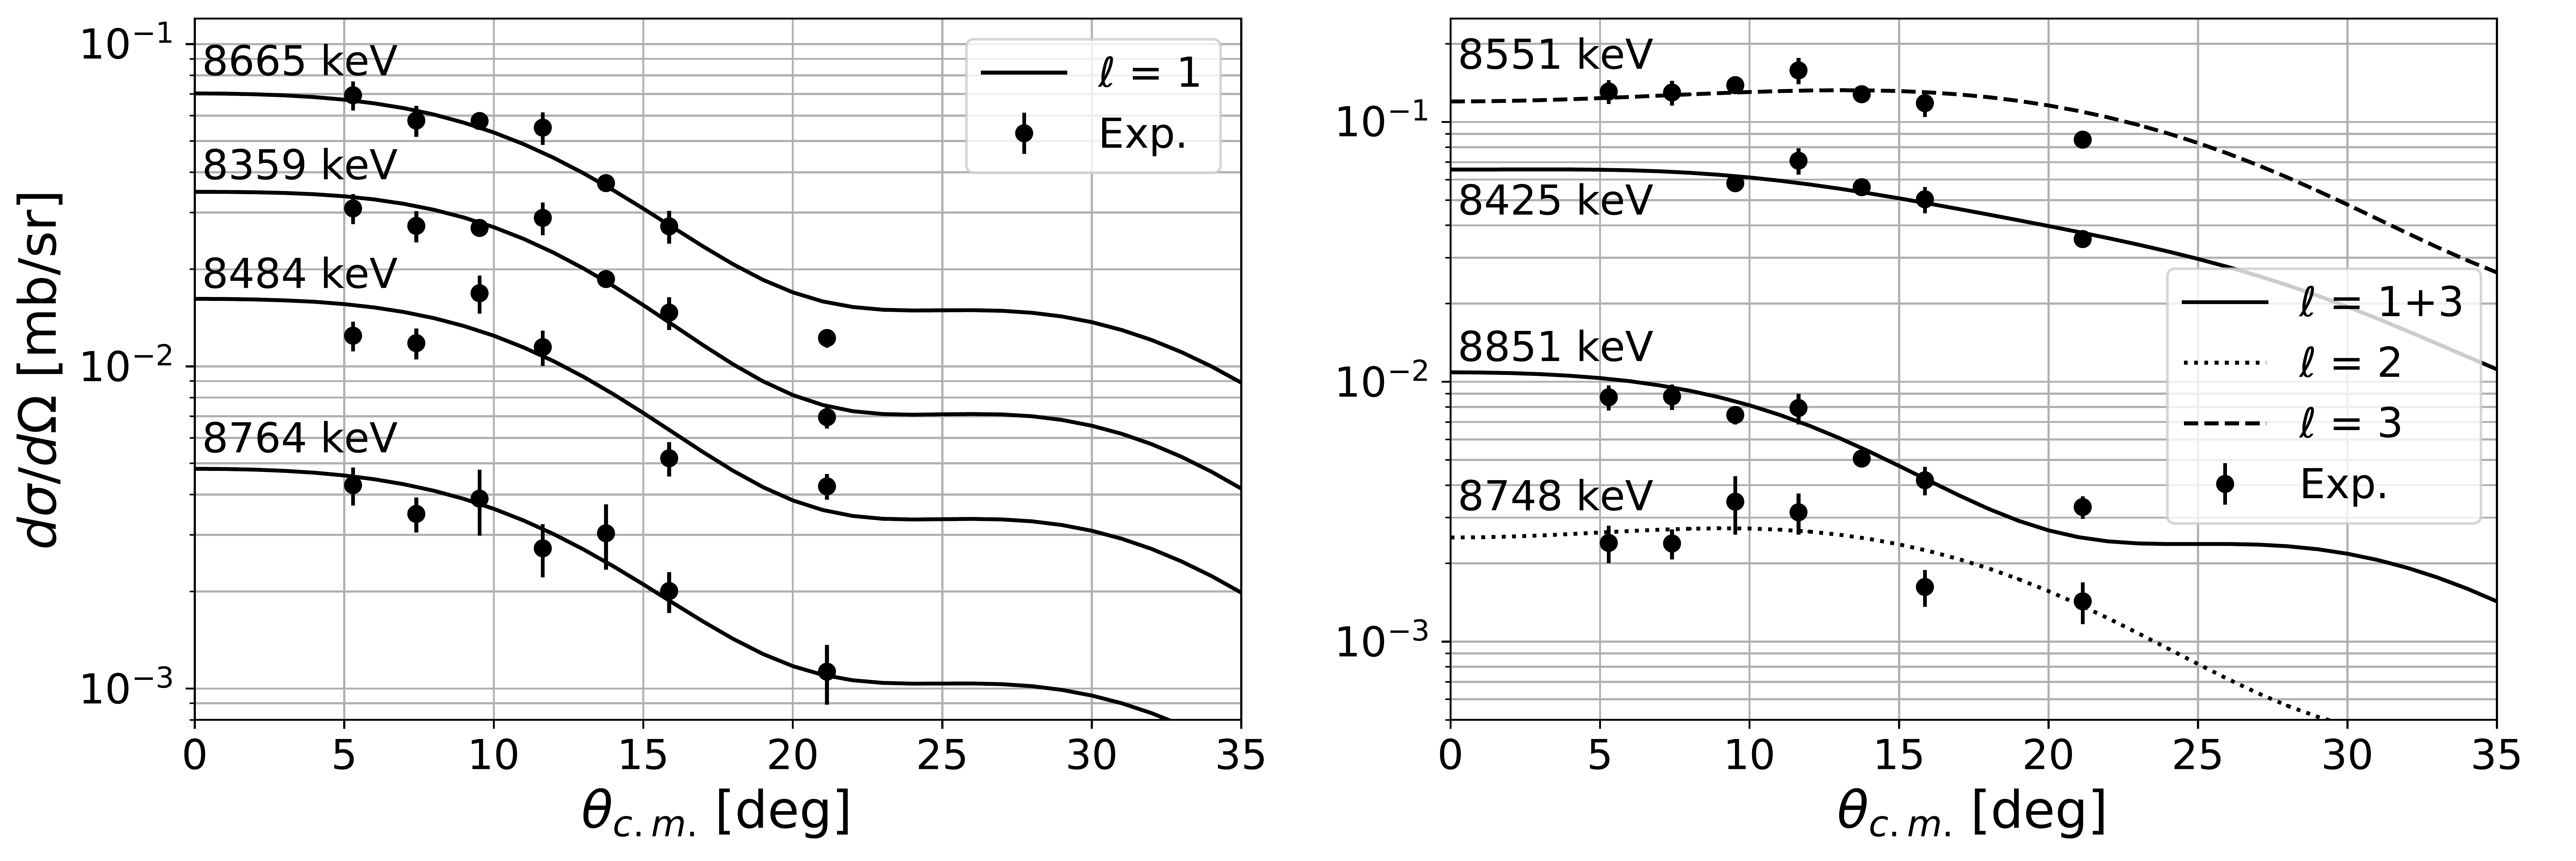
\includegraphics[width=6.5in]{Chapter-6/figs/unbound.png}
\caption{\label{fig:unbound_l}Differential cross-sections of unbound $^{40}\mathrm{Ca}$ states below 8935 keV observed in the present experiment. The left panel shows the $l=1$ distributions, while the right panel shows all other distributions. The experimental data were normalized to the Si detector telescope yield, as described in the text, and further scaling for illustration purposes was not necessary. The zero-range DWBA model curves were computed using the nuclear reaction code, \texttt{Fresco} \cite{Thompson1988,Fresco}.}
\end{figure*}

\subsection{Oxidized Targets} \label{subsec:oxidized_cs}

% Effects oxidized targets have on the cross-section
% Adding a 10% scatter? Any corrections? Revisit python notebook to see what I did

\subsection{Spectroscopic Factors from DWBA Models} \label{subsec:DWBA_Spec}



\subsection{Proton Partial Widths} \label{subsec:partial_widths}



%%%%%%%%%%%%%%%%%%%%%%%%%%%%%%%%%%%%%%%%%%%%%%%%%%%%%%%%%%%%%%%%%%%%%%%%%%%%%%%%%%%%%%%%%%%%%
\section{New $^{39}\mathrm{\textbf{K}}(p,\gamma)^{40}\mathrm{\textbf{Ca}}$ Reaction Rate}

The Monte Carlo reaction rate code, \texttt{RatesMC} \cite{Longland2010a,RatesMC}, was used to calculate a new $^{39}\mathrm{K}(p, \gamma)^{40}\mathrm{Ca}$ reaction rate probability density from the resonance energies and proton partial-widths reported in Sections \ref{subsec:cal} and \ref{subsec:partial_widths}, respectively. Among the states observed in the $^{39}\mathrm{K}(^{3}\mathrm{He},d)^{40}\mathrm{Ca}$ experiment, only those that do not already have a directly measured $^{39}\mathrm{K}(p, \gamma)^{40}\mathrm{Ca}$ resonance strength from Refs. \cite{Kikstra1990,Cheng1981,Leenhouts1966} were modified from the most recent reaction rate evaluation of Ref. \cite{Longland2018}. That is, the only resonance strengths and resonance energies that were updated from those in Ref. \cite{Longland2018} are below the $E_{x} = 8935$ keV ($E^{\mathrm{c.m.}}_{r} = 606$ keV) resonance. Otherwise, the expectation values and variances of the $^{39}\mathrm{K}(p, \gamma)^{40}\mathrm{Ca}$ experiments \cite{Kikstra1990,Cheng1981,Leenhouts1966} are adopted from Ref. \cite{Longland2018}.

% Everything above this is up-to-date for this thesis (Except 6.7 and 6.8)

The new reaction rate is compared with that of Ref. \cite{Longland2018} in Fig. \ref{fig:rateCompare}. The solid line and blue band represent the median, recommended rate and the $1\sigma$ confidence interval of this work, respectively. The dotted line and gray band represent that of Ref. \cite{Longland2018}, except with resonance energies calculated using $S_{p} = 8328.18(2)$ keV from Ref. \cite{Wang2021} for consistency, but with marginal effect. Both reaction rates are normalized to the median, recommended rate of Ref. \cite{Longland2018}. %,where the bands represent the 1$\sigma$ confidence interval of each Monte Carlo calculation. 

As mentioned previously, the large uncertainty in Ref. \cite{Longland2018}, between about 50 MK and 200 MK, corresponds to most of the relevant temperatures that reproduce the Mg--K anticorrelation in the globular cluster NGC 2419 \cite{Iliadis2016}. 
%Above 20 MK, the region with the largest uncertainty in Ref. \cite{Longland2018}, between about 50 MK and 200 MK, corresponds to most of the relevant temperatures that reproduce the Mg--K anticorrelation in the globular cluster NGC 2419 \cite{Iliadis2016}.
Fig. \ref{fig:rateCompare} illustrates that the new reaction rate increases significantly in this range, particularly at 70 MK where the median rate is a factor of 13 larger than the rate of Ref. \cite{Longland2018}. The $1\sigma$ width is also significantly reduced in this region, from a factor of 84 at 80 MK to just a factor of 2, a reduction of a factor of 42.

Our new determination of $(2J+1)\Gamma_{p}$ for the 154 keV resonance is primarily responsible for the increase in the rate and decrease in the uncertainty between about 55 MK and 110 MK. Similar effects occur between about 20 MK and 55 MK, primarily from our $l=1+3$ assignment of the 96 keV resonance, which has replaced the $l=3$ assignment by the other $(^{3}\mathrm{He}, d)$ measurements in this calculation. The $(d,n)$ measurement of Ref. \cite{Fuchs1969} is in agreement with the $l=1+3$ assignment for this resonance. Note that using the previous $l=3$ assignment has a negligible effect on the results mentioned above at 70 and 80 MK. Our $(2J+1)\Gamma_{p}$ determination for the 29 keV resonance is responsible for the rate increase below 20 MK. The smaller effects above 110 MK are from a combination of the 335 keV, 415 keV, 439 keV, and 521 keV resonances, the latter three of which have replaced $(2J+1)\Gamma_{p}$ upper limits in Ref. \cite{Longland2018}.

\subsection{Resonance Contributions}

\begin{figure}[t]
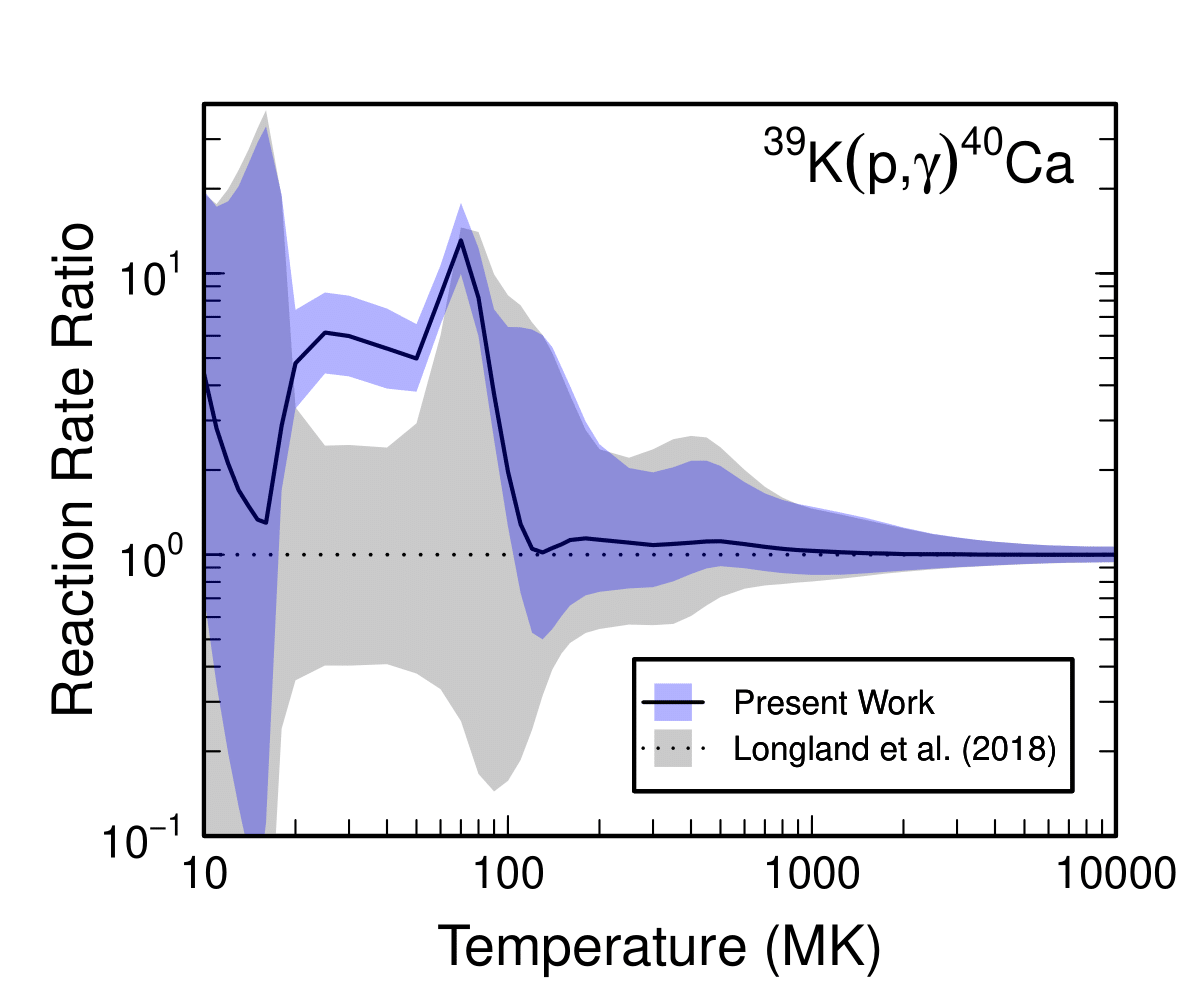
\includegraphics[width=6.5in]{Chapter-6/figs/rateCompare.png} % 6.5 in is exact page width (8.5 in) minus the 1 in margins. Height scaled automatically to keep aspect ratio.
\caption{\label{fig:rateCompare}Comparison between the $^{39}\mathrm{K}(p, \gamma)^{40}\mathrm{Ca}$ reaction rate using the proton partial-widths and resonance energies of the present experiment (solid line, blue band) and the most recent evaluation of Ref. \cite{Longland2018} (dotted line, gray band). The reaction rate ratio is taken with respect to the median, recommended rate of Ref. \cite{Longland2018} for both calculations. The $1\sigma$ uncertainty bands are shown.}
\end{figure}

\begin{figure}[t]
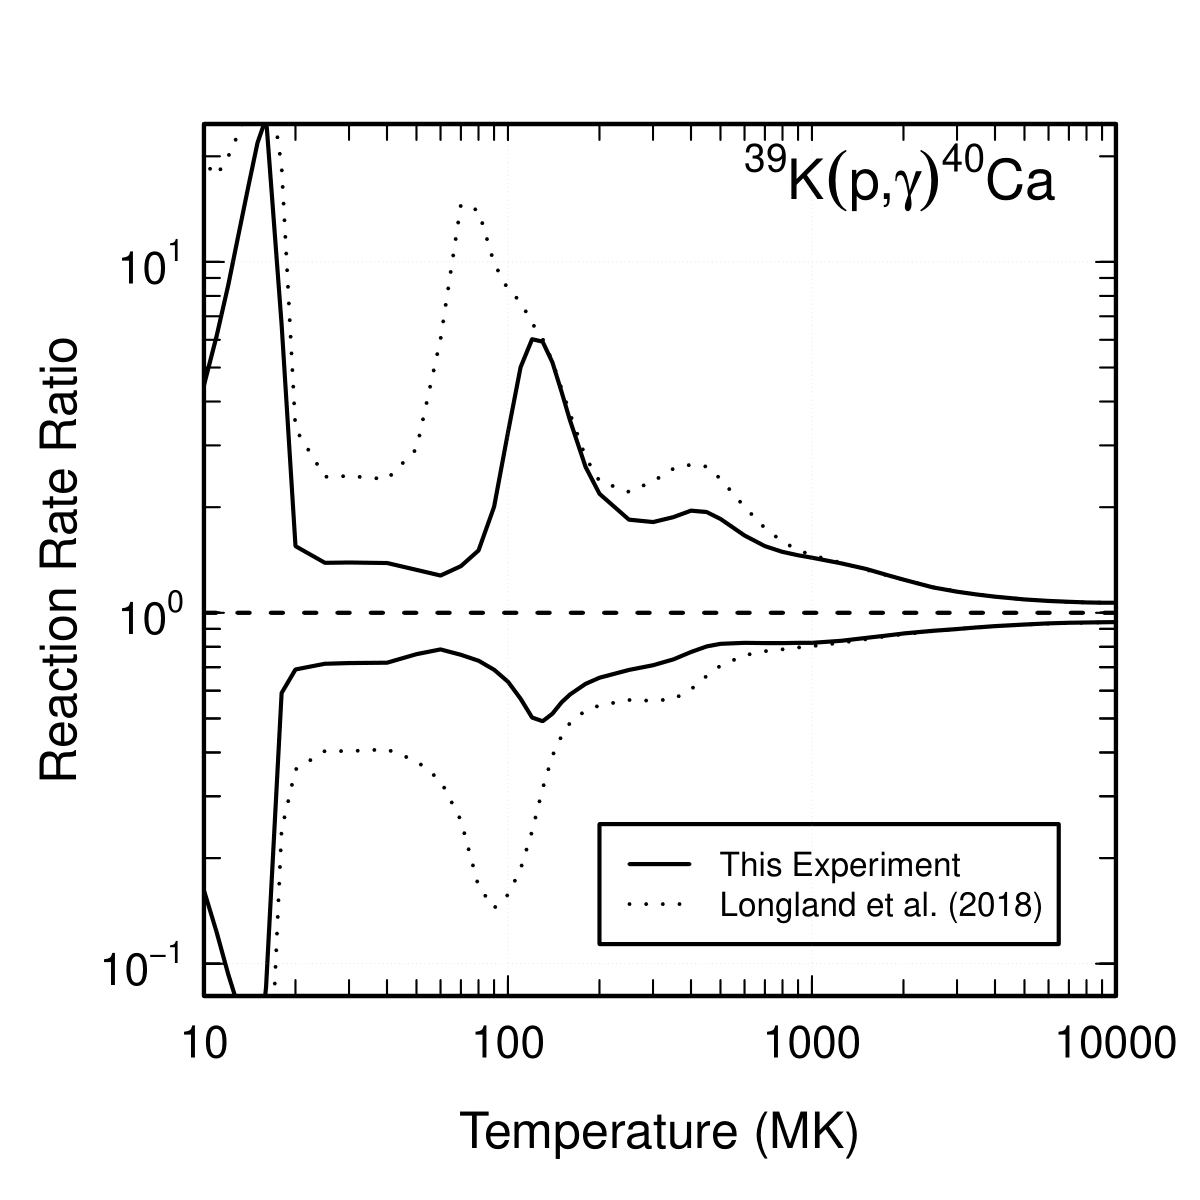
\includegraphics[width=6.5in]{Chapter-6/figs/uncCompare.png} % 6.5 in is exact page width (8.5 in) minus the 1 in margins. Height scaled automatically to keep aspect ratio.
\caption{\label{fig:uncCompare}Comparison between the $^{39}\mathrm{K}(p, \gamma)^{40}\mathrm{Ca}$ reaction rate uncertainty using the proton partial-widths and resonance energies of the present experiment (solid band) and the most recent evaluation of Ref. \cite{Longland2018} (dotted band). Each reaction rate ratio is taken with respect to their own median, recommended rate. The $1\sigma$ uncertainty bands are shown.}
\end{figure}

\begin{figure}[t]
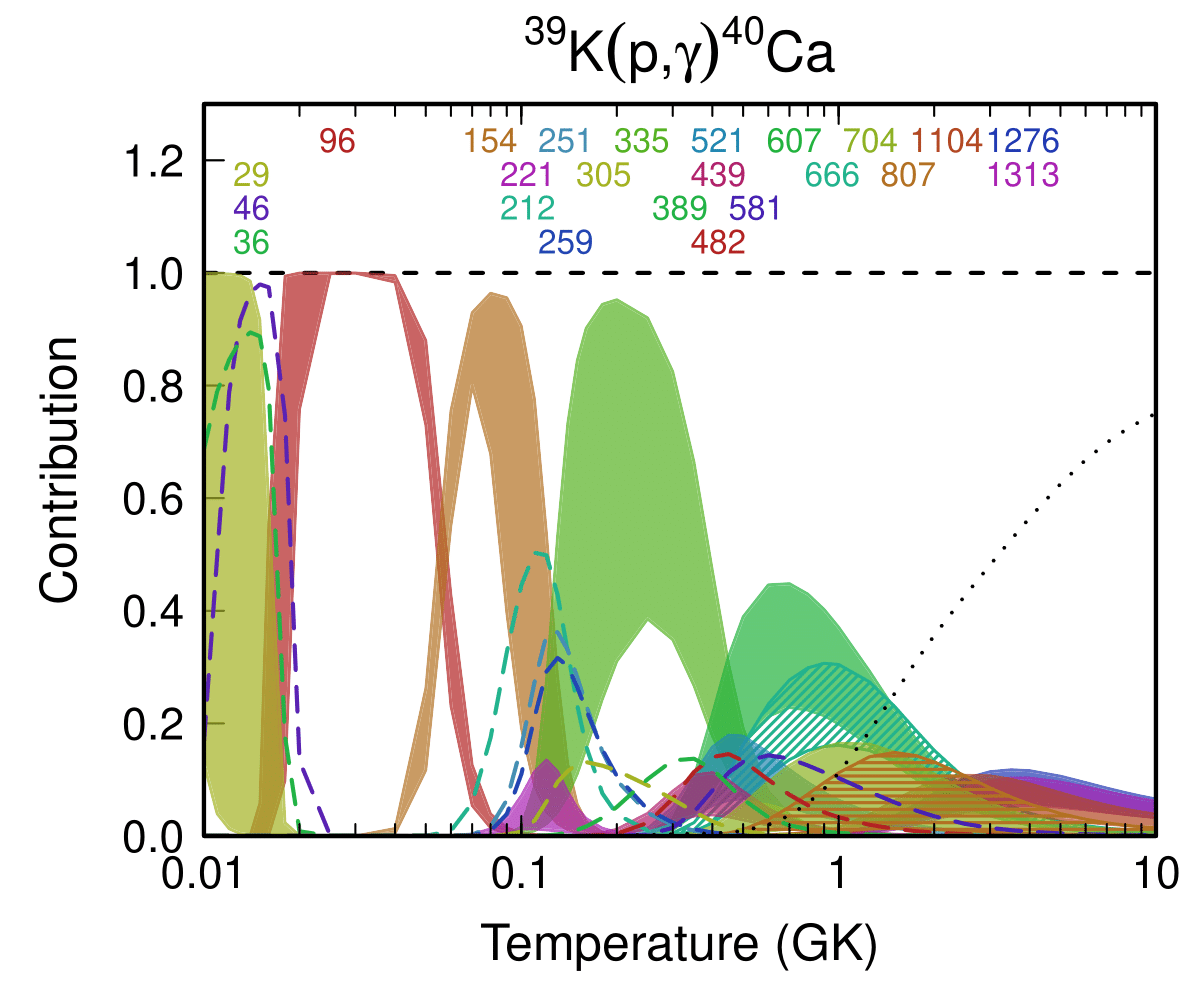
\includegraphics[width=6.5in]{Chapter-6/figs/Contrib_Fox.png} % 6.5 in is exact page width (8.5 in) minus the 1 in margins. Height scaled automatically to keep aspect ratio.
\caption{\label{fig:contrib}Individual resonance contributions to the $^{39}\mathrm{K}(p,\gamma)^{40}\mathrm{Ca}$ reaction rate, where a value of 1.0 implies that the given resonance contributes 100$\%$ to the reaction rate at that temperature. The labels correspond to center-of-mass resonance energies in keV. Resonances with shading or hatched lines have been measured and are shown with their $1\sigma$ uncertainty bands. Resonances with a single, dashed line are upper limit calculations and show their 84$\%$ $1\sigma$ value, for clarity. The resonances displayed are those that individually account for at least 10$\%$ of the total reaction rate at their corresponding temperatures. The remaining summed resonance contributions are represented by the dotted line.}
\end{figure}

%%%%%%%%%%%%%%%%%%%%%%%%%%%%%%%%%%%%%%%%%%%%%%%%%%%%%%%%%%%%%%%%%%%%%%%%%%%%%%%%%%%%%%%%%%%%%
\section{Potassium Abundance in Reaction Network Calculations}


%%%%%%%%%%%%%%%%%%%%%%%%%%%%%%%%%%%%%%%%%%%%%%%%%%%%%%%%%%%%%%%%%%%%%%%%%%%%%%%%%%%%%%%%%%%%%
\section{Conclusions}


%%%%%%%%%%%%%%%%%%%%%%%%%%%%%%%%%%%%%%%%%%%%%%%%%%%%%%%%%%%%%%%%%%%%%%%%%%%%%%%%%%%%%%%%%%%%%
